\documentclass[12pt]{graphicsclass}
\usepackage[utf8]{inputenc}
\usepackage{palatino}
\usepackage{amsmath}
\usepackage{amssymb} 
\usepackage{graphicx}
\usepackage[labelfont=bf]{caption}
\usepackage{subcaption}
\usepackage{setspace}
\captionsetup[table]{font = {stretch=1.35}}
\captionsetup[figure]{font = {stretch=1.35}}
\usepackage[margin=1in]{geometry}
\linespread{1.6}
\usepackage[hidelinks]{hyperref}
\usepackage{cite}
\usepackage{xcolor}
\usepackage{overpic}
\usepackage[all]{nowidow}

\usepackage{afterpage}
\usepackage{listings}
\usepackage{float}
\usepackage{svg}
\usepackage{url}

\usepackage{color, colortbl}
\usepackage{booktabs}

\usepackage{courier}

\lstdefinelanguage{JavaScript}{
  keywords={typeof, new, true, false, catch, function, return, null, catch, switch, var, if, in, while, do, else, case, break},
  ndkeywords={class, export, boolean, throw, implements, import, this},
  sensitive=false,
  comment=[l]{//},
  morecomment=[s]{/*}{*/},
  morestring=[b]',
  morestring=[b]"
}

\lstdefinelanguage{SableWasmMIR}{
  alsoletter={.:},
  keywords={function, memory, table, global, var, const},
  ndkeywords={i32, i64, f32, f64, v128,
    int.eq, i32.const, i64.const,
    int.add, memory.guard,
    load.32, load.16, load.64, 
    cast, 
    local.get, 
    call,
    local.set,
    br, br.cond, br.table, ret, phi, 
    v128.int.extract, v128.int.insert, v128.int.splat,
    v128.int.mul,
    store.32, store.16,
    int.lt.u, int.rem.s, int.eqz
  }
}

\title{
{SABLEWASM: A STATIC COMPILER AND RUNTIME FOR WEBASSEMBLY}\\~\\~\\
{\large Hongji Chen, School of Computer Science \\ 
	McGill University, Montreal \\ 
	August, 2021 \\~\\~\\
	A thesis submitted to McGill University in partial fulfillment of the 
	requirements of the degree of \\~\\ Master of Computer Science }\\~\\
}

\setcounter{page}{2}\renewcommand{\thepage}{\roman{page}}

\author{\textcopyright Hongji Chen, 2021}
\date{}

\begin{document}
\maketitle


\chapter*{Abstract}
\label{sec:engAbstract}
\addcontentsline{toc}{section}{\nameref{sec:engAbstract}}
\emph{WebAssembly} is a relatively new language, introduced to improve the
performance of compute-intensive workloads in web-based applications. It offers
a compact binary bytecode intended to allow for fast compilation and improved
optimization opportunities over dynamic web languages like JavaScript. These
properties, however, also make it an interesting target for static execution,
enabling web code to run outside of a browser as well as within it. In this
thesis, we describe \emph{SableWasm}, a static, multi-pass compiler system that
translates sandboxed WebAssembly applications to native shared libraries. Our
work covers several different aspects of compiler design. First, we provide an
efficient and extensible WebAssembly module parsing and validation framework,
with improved execution speed and memory footprint compared to the reference
baseline. We then define a middle-level intermediate representation and build
an analysis and transformation framework. We explore several classic data-flow
analyses, such as dominator-tree construction within the framework, and
additionally identify several WebAssembly specific optimization opportunities,
which we address through custom transformation passes. SableWasm also
incorporates several in-progress extension proposals including the SIMD vector
operation extension. Optimized intermediate code is then converted to native
code through a backend implementation with the help of the LLVM compiler
framework and a runtime that enables C/C++ programs to interact with the
WebAssembly module directly. Finally, we evaluate SableWasm by benchmarking
against several well-known testing suites and observe performance improvement
compared to the baseline implementation.

\chapter*{Abrégé}
\label{sec:frAbstract}
\addcontentsline{toc}{section}{\nameref{sec:frAbstract}}
\begin{spacing}{1.4}
    \textit{WebAssembly} est un langage relativement nouveau, introduit pour améliorer les performances des charges de travail gourmandes en calcul dans les applications Web. Il offre un bytecode binaire compact destiné à permettre une compilation rapide et des opportunités d'optimisation améliorées sur des langages Web dynamiques comme JavaScript. Ces propriétés, cependant, en font également une cible intéressante pour l'exécution statique, permettant au code Web de s'exécuter en dehors d'un navigateur ainsi que dans celui-ci. Dans cette thèse, nous décrivons \textit{SableWasm}, un système de compilation statique à passes multiples qui traduit les applications WebAssembly en bac à sable en bibliothèques partagées natives. Notre travail couvre plusieurs aspects différents de la conception du compilateur. Premièrement, nous fournissons un cadre d'analyse et de validation de module WebAssembly efficace et extensible, avec une vitesse d'exécution et une empreinte mémoire améliorées par rapport à la ligne de base de référence. Nous définissons ensuite une représentation intermédiaire de niveau intermédiaire et construisons un cadre d'analyse et de transformation. Nous explorons plusieurs analyses classiques de flux de données, telles que la construction de l'arbre dominateur et la numérotation des valeurs locales dans le cadre, et identifions en outre plusieurs opportunités d'optimisation spécifiques à WebAssembly, que nous abordons via des passes de transformation personnalisées, telles que l'élimination des variables locales redondantes. SableWasm intègre également plusieurs propositions d'extension en cours, y compris l'extension d'opération de vecteur SIMD. Le code intermédiaire optimisé est ensuite converti en code natif via une implémentation backend à l'aide du framework de compilateur LLVM et d'un runtime qui permet aux programmes C/C++ d'interagir directement avec le module WebAssembly. Enfin, nous évaluons SableWasm en comparant plusieurs suites de tests bien connues et observons une amélioration des performances par rapport à l'implémentation de base.
\end{spacing}

\chapter*{Acknowledgements}
\label{sec:ded}
\addcontentsline{toc}{section}{\nameref{sec:ded}}
First, I would like to extend my deepest gratitude to Professor Clark Verbrugge.
The work would not have been possible without his support and advice, especially
during a global pandemic. Secondly, I would like to thank Professor
Laurie Hendren for her guidance in the field of compiler design in my early days
as an undergraduate student. Finally, I would like to thank my colleagues and
friends, especially my Sable lab mates, for their encouragement throughout the
entire thesis journey.

\tableofcontents
\listoffigures %
\addcontentsline{toc}{section}{\listfigurename}
\listoftables
\addcontentsline{toc}{section}{\listtablename}

\clearpage
\pagenumbering{arabic} % restart page numbers at one, now in arabic style

%% start of chapters
\chapter{Introduction}
\label{chapter:introduction}

Web-based applications have grown in popularity in recent years. From the early
days of simple web applets to current full-blown programs, their codebase's
complexity and size has grown rapidly. Due to the design of most browsers,
programmers have to choose JavaScript or its dialects to implement them. This
approach is quite successful; however, it still leaves several problems
unsolved. First, JavaScript is a scripting language and employs many dynamic
features that prevent backend runtime environment from efficient execution,
such as dynamic typing. Additionally, when porting existing applications to
JavaScript, especially those with a large codebase where manually translating
source code line-by-line is not feasible, a nontrivial source-to-source
compiler is needed due to the structural difference between native binaries and
JavaScript source codes.

To address these problems, the WebAssembly working group was established in
2017, and purposed a new standard for distributing applications over the
Internet. WebAssembly focuses on safety, performance, portability and module
compactness. These properties also make it an interesting target for static
execution, enabling sandboxed applications outside of browsers. To this end,
the WebAssembly community further designed the WebAssembly System Interface
(WASI), which provides a standardized interface for WebAssembly modules to
access native features such as the file system.

WebAssembly is also an evolving language. Although the WebAssembly community
has published the minimum viable product (MVP) WebAssembly, the community is
still actively proposing and experimenting with new language features, such as
exception handling and garbage collection. These additional language features
are proposed in language extension proposals that modify the current WebAssembly
specification syntactically and semantically. Thus, a well-designed WebAssembly
runtime environment system should be modular and extensible, leaving space for
future design changes.

\section{Contribution}

\begin{figure}
    \centering
    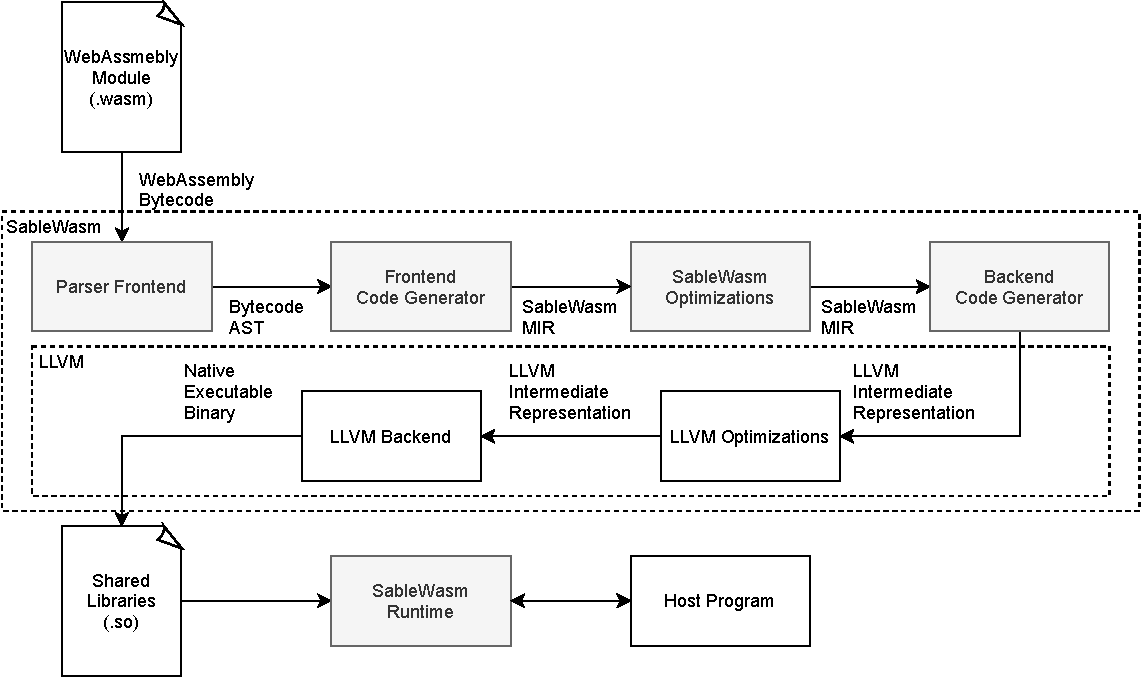
\includegraphics[width=\textwidth]{Images/design}
    \caption{The SableWasm compiler and runtime}
    \label{fig:design}
\end{figure}

This thesis aims to design and implement a runtime environment that enables
WebAssembly to run outside of the browser. To this end, this thesis makes three
major contributions. Figure~\ref{fig:design} illustrates the SableWasm compiler
and runtime system. We mark our contributions in this thesis as shaded boxes
in the figure.

\paragraph{Implementing a WebAssembly runtime system}
Our first contribution is a standalone WebAssembly runtime environment with
support for the WebAssembly System Interface (WASI). We first start by
implementing a custom extensible parser frontend for WebAssembly binary format,
shown as the `Parser Frontend' in figure~\ref{fig:design}.
We then define a `middle-level' representation (MIR) for SableWasm.
To match modern hardware, SableWasm MIR is a register-based
\emph{control flow graph} representation of the program, while, on the
other hand, WebAssembly operates over a stack-based virtual machine. Hence,
translating between them is nontrivial. Therefore, we design and implement a
frontend code generator that lowers WebAssembly bytecode into SableWasm MIR,
shown as the `Frontend Code Generator' in figure~\ref{fig:design}.
SableWasm MIR plays a critical role in the SableWasm system. First, it
provides a middle ground where we implement an extensible and straightforward
optimization framework. With the help of the framework, we experiment with
several analyses and optimizations on SableWasm MIR. Second,
SableWasm MIR also separates the frontend from the backend. Currently, we
implement an ahead-of-time (AOT) compiler backend using the LLVM compiler
infrastructure \cite{llvm-thesis}, shown as the `Backend Code Generator' in
figure~\ref{fig:design}. However, there are several challenges when lowering
SableWasm MIR into LLVM intermediate representation. For example, SableWasm MIR,
similar to WebAssembly bytecode, utilizes several abstract high-level concepts
such as linear memory and indirect function calls. These operations cannot be
trivially mapped to LLVM instructions and require runtime library support.
Hence, the last component of SableWasm is a runtime library that provides
builtin runtime functions for the generated modules and defines an easy-to-use
interface for the host system, shown as the `SableWasm Runtime' in
figure~\ref{fig:design}.

\paragraph{Adding support for WebAssembly extensions}
Our second contribution in this thesis is to experiment and adopt several
in-progress WebAssembly language extensions. SableWasm is designed to be
extensible and currently implements four post-MVP WebAssembly features. The
most interesting one among them is perhaps the fixed-width SIMD operation
extension which defines vector-based operations that can operate on multiple
data simultaneously, packed into special vector registers and supported by
modern hardware. The SIMD extension in WebAssembly
introduces one additional value type and approximately 240
new instructions to the specification. As we have discussed earlier in this
section, SableWasm MIR provides a middle ground where we perform optimization
on the program. Therefore, we would like to keep the size of the SableWasm MIR
instruction set simple. To achieve this goal, we carefully design a set of
reduction patterns in the frontend code generator that significantly reduce the
number of instructions needed. We also generalize our backend code generator
that targets LLVM by emitting corresponding vector operation instructions.

\paragraph{Evaluating system performance}
Our last contribution in this thesis is to investigate how SableWasm performs
and the factors that affect the performance. Here we focus on three research
questions: First, how does SableWasm perform comparing to other existing
WebAssembly runtime implementations? Second, does optimization over the input
WebAssembly modules affect SableWasm's overall performance? Finally, does the
SIMD operation extension bring performance improvement to the system? To answer
these questions, we analyze the performance of three well-known benchmark
suites, Polybench \cite{polybench}, Ostrich \cite{ostrich}, and NPB \cite{npb}.
We also examine generated LLVM intermediate representations in SableWasm to
search for factors contributing to the slow down in the system.

\section{Thesis outline}

This thesis consists of nine chapters in total, including the introduction
chapter.
Chapter~\ref{chapter:background} discusses the background information that helps
the understanding rest of the thesis. It first presents the motivation for
WebAssembly and WebAssembly System Interface (WASI), followed by a brief
overview of the LLVM intermediate representation.
Chapter~\ref{chapter:frontend} to chapter~\ref{chapter:backend-and-runtime}
discusses the design of implementation of the SableWasm system.
Chapter~\ref{chapter:frontend} starts with presenting the custom extensible and
efficient parser frontend for WebAssembly binary format.
Chapter~\ref{chapter:mir-design} continues the discussion of SableWasm by
describing SableWasm MIR's design.
Chapter~\ref{chapter:mir-translation-optimization} discusses the code
generating strategies used when lowering WebAssembly bytecode to SableWasm MIR
and the optimization framework.
Chapter~\ref{chapter:mir-translation-optimization} also presents several
optimization passes we experimented with the framework, such as control flow
graph simplification and type inference.
Chapter~\ref{chapter:backend-and-runtime} illustrates the last component of
SableWasm, the LLVM backend and the runtime support library.
In chapter~\ref{chapter:evaluation}, we investigate the performance of SableWasm
by presenting benchmark results and discussing several possible theories for the
slowdown.
Finally, chapter~\ref{chapter:related-work} discusses related work and
chapter~\ref{chapter:conclusion} presents our conclusion along with future work.
\chapter{Background}

This chapter provides background information that helps to understand the
thesis. We first revisit the rise of asm.js and its toolchain, Emscripten,
followed by an introduction to WebAssembly and its standardized native system
interface WASI. Finally, we will give a brief overview of the LLVM compilation
framework.

\section{Emscripten and Asm.js}

In the past decade, web-based applications are gaining popularity, and due to
the design of most browsers, programmers tend to choose JavaScript or its
dialects to implement them. One natural problem is how to compile programs that
target the native platform to run over the internet. Making the situation more
challenging, programs with a large codebase, for example games that require
complex video and physical computation, are nearly impossible to translate
line-by-line manually. In 2010, Alon Zakai started the first attempt at
translating source code that targets native platforms into JavaScript
\cite{8118483}. After two years of development, he published Emscripten that
translates LLVM intermediate representation into asm.js, a JavaScript subset
\cite{10.1145/2048147.2048224}. An asm.js program shares a similar programming
model to that which one would expect on the native platform. The detailed asm.js
specification is available on the official website
\footnote{asm.js specification: \url{http://asmjs.org/spec/latest/}}.
We will visit several critical features in asm.js with examples in
figure~\ref{fig:adler-32} (page~\pageref{fig:adler-32}). These examples are
implementations of the Adler-32 hashing algorithm used in ZLib compression
library \cite{adler32-paper} \footnote{Revisiting Fletcher and Adler Checksums:
  \\\url{http://www.zlib.net/maxino06\_fletcher-adler.pdf}}, in both C and its
corresponding generated asm.js with Emscripten.

\begin{figure}
  \centering
  \begin{subfigure}{\textwidth}
    \lstinputlisting[
      language=C,
      basicstyle=\linespread{0.4}\small\ttfamily, numbers=left
    ]{Code/adler32.c}
    \caption{C}
    \label{fig:adler-32-c}
  \end{subfigure}
  \begin{subfigure}{\textwidth}
    \lstinputlisting[
      language=JavaScript,
      basicstyle=\linespread{0.4}\small\ttfamily, numbers=left
    ]{Code/adler32.js}
    \caption{asm.js}
    \label{fig:adler-32-asmjs}
  \end{subfigure}
  \begin{subfigure}{\textwidth}
    \lstinputlisting[
      basicstyle=\linespread{0.4}\small\ttfamily,
      numbers=left
    ]{Code/adler32.wat}
    \caption{Text-format WebAssembly}
    \label{fig:adler-32-webassembly}
  \end{subfigure}
  \caption{Adler 32 in C, asm.js and text-format WebAssembly}
  \label{fig:adler-32}
\end{figure}

\paragraph{Function prologue and type annotation}
JavaScript is a dynamically typed language. Hence, a proper implementation needs
to verify the types of variables when needed. Although several optimization
techniques can eliminate some of the checks and improve the execution
performance, such language features can still incur a significant performance
loss. Asm.js adds type annotations to function parameters and expressions to
address this problem. In figure~\ref{fig:adler-32-asmjs}, Emscripten generates
parameter annotations for parameters \texttt{\$0\_1} and \texttt{\$0\_2} at
line $2$ and line $3$ respectively. The trailing bitwise `or' operation against
zero hints that both arguments are integral values since bitwise operations are
only defined for integral values in JavaScript. Emscripten also annotates
float-point numbers with the unary positive operation, `+', which we do not show
in the example. A system that supports asm.js directly can quickly recover the
type information from the annotations, which, in theory, can improve both the
compilation and execution performance. On the other hand, for a system that does
not recognize asm.js, the program above is still a valid JavaScript program, and
the type annotations ensure the correct semantics for numeric operations.

\paragraph{Control flow}
LLVM employs a register-based intermediate representation with a
\emph{control flow graph} (CFG). However, JavaScript uses structured control
flow and does not allow arbitrary jump statements similar to one would expect
in C. Hence, when translating LLVM IR to asm.js, Emscripten mimics the branch
instructions between basic blocks in the generated code with JavaScript
control-flow statements. Emscripten uses a pattern-based translation and
classifies control flow changes into three categories.
In figure~\ref{fig:adler-32-asmjs}, we demonstrate two of the three
control-flow structures, \emph{if} and \emph{loop}, at line $6$ and line $7$
respectively. Asm.js also has a third control flow structure, \emph{block},
which we do not show in the example. A \emph{block} structure is similar to a
\emph{loop} structure and can be translated to a while loop with an always-false
condition. A jump instruction referring to the \emph{block} is equivalent to a
break statement in this case. WebAssembly adopts a similar design, and we will
revisit this in the later section with more details.

\paragraph{Byte array as heap}
Emscripten uses multiple typed array views that share a single underlying byte
array buffer to simulate the heap in a native programming model.
In figure~\ref{fig:adler-32-asmjs}, the asm.js example uses \texttt{HEAPU8}, an
unsigned byte view over the byte array at line $8$, to access the data passed by
the pointer via the first argument. Asm.js also offers other array views such
as \texttt{HEAPI32} and \texttt{HEAPF32} which allows programs to access 32-bit
signed integers and single-precision floating-point numbers on the heap. This
technique also inspires the linear memory design in WebAssembly, which we will
discuss later in the chapter with more details.

Emscripten is quite successful. Experiment results show that it can port most of
the C/C++ programs of non-trivial code size to the web with approximately
50-67\% of native performance
\footnote{Alon Zakai's presentation on Emscripten at CppCon:
  \\\url{https://kripken.github.io/mloc_emscripten_talk/cppcon.html}}
without any missing significant features.

\section{WebAssembly}

Although Emscripten with asm.js is successful, there are still several problems
that remain unaddressed. One of them is the parsing overhead. As asm.js is a
strict subset of JavaScript, parsing the generated program is a non-trivial task
due to the complexity of JavaScript grammar. Additionally, because Emscripten
emits generated programs in asm.js, the output size grows significantly faster
than the native binary. Another problem regards the generated programs' safety,
especially when running an untrusted module received over the internet. In 2017,
the WebAssembly community established and proposed a new standard for
distributing programs over the internet to address these problems. The design of
WebAssembly focuses on safety, performance, portability, and compactness. The
introduction paper describes the detailed structure, validation rules
\cite{10.1145/3167082}, and execution semantics of WebAssembly
\cite{10.1145/3062341.3062363}. Here we will only visit some of the key points
that help understand the rest of the thesis. In
figure~\ref{fig:adler-32-webassembly} we also present a simple WebAssembly
program that implements the Adler32 hashing.

\paragraph{Module structure}
WebAssembly modules can have four different kinds of entities: \emph{functions},
\emph{tables}, \emph{linear memories}, and \emph{globals}. Modules are also able
to import and export entities by names. In
figure~\ref{fig:adler-32-webassembly}, we define a \emph{function} and a
\emph{linear memory} and export them under name \texttt{adler32} and
\texttt{memory} respectively. WebAssembly functions can define an arbitrary
number of local variables and possibly an empty sequence of instructions as the
body. All instruction operates over an implicitly declared stack. The
control-flow will return from the function by either a \texttt{return}
instruction or reaching the end of the body. WebAssembly linear memories have
bounds consisting of a pair of integers, representing the lower bound and upper
bound respectively, \footnote{The upper bound is optional} in units of $16$-KiB
pages. In figure~\ref{fig:adler-32-webassembly}, at line $21$, we defined a
linear memory with a minimal size of $32$-KiB. WebAssembly linear memory can
also associate with zero or multiple \emph{data} segments. Each \emph{data}
segment contains a constant evaluated expression, representing the
initialization offset, and a sequence of bytes that the runtime environment will
copy from. WebAssembly tables are similar to memories, but they store function
pointers instead of bytes. A \emph{table} has a type that consists of an upper
and lower bound similar to \emph{memory}, as well as a function type indicating
the type of the function pointers allowed \footnote{Currently, the function type
  must be \texttt{funcref} which is a union type of all possible function
  types.}. WebAssembly tables also introduce their initializer, \emph{element}
segments. The \emph{element} segment is similar to the \emph{data} segment, but
it initializes function pointers instead of bytes. Another difference between
linear memories and indirect tables is that indirect tables are immutable after
initialization to ensure the module's safety \footnote{This is subject to change
  in the reference type extension}.

\paragraph{Linear memory}
Similar to asm.js, WebAssembly programs can access one or multiple
\emph{linear memories} \footnote{In the current version of WebAssembly, at most
  one linear memory is allowed within a single module}. The memory is unmanaged,
and it is the program's responsibility to handle the layout correctly. The
program can grow the \emph{linear memory} if needed via the \texttt{memory.grow}
instruction; however, the runtime environment is not obligated to increase the
\emph{linear memory}. The program can check the result of the command via the
instruction's return value. Asm.js also allows the growth of the heap byte
array. However, due to the limitations of JavaScript, this operation is usually
quite expensive, as there is no efficient \texttt{realloc} algorithm provided in
JavaScript, and it requires allocating a byte array with a larger capacity and
copying byte-by-byte. WebAssembly specification does not impose requirements on
the time complexity to grow the linear memory, yet it encourages any
implementation to avoid copying.  Unlike native heap memory, there is no
alignment requirement on load-store instructions; i.e., load-store can start at
any byte in the memory with the probable additional cost for unaligned access.
However, there are boundary checks applied to the linear memory. Any
out-of-bound access will result in a runtime panic. Additionally, WebAssembly
specification requires any runtime environment implementation to
zero-initialize the linear memory.

\paragraph{Indirect table}
Asm.js represents function pointers using first-class function values, thanks to
JavaScript. However, in WebAssembly, every entity is referred to with indices
representing references, and value types only consist of integral types and
floating-point types \footnote{WebAssembly may introduce more primitive value
  types in the future.}. Hence, we need something creative to implement the
function pointers in WebAssembly. The solution utilizes one special instruction
\texttt{call\_indirect} and indirect tables. During module initialization, the
runtime environment will initialize the indirect table according to the
\emph{element} section. Each \texttt{call\_indirect} instruction associates
with an index and an expecting type. The runtime environment will perform both
a validity check on the index and a type check with the expecting type's help.
Unlike the memory, the indirect table is not growable at runtime and currently
is immutable once the initialization phase is complete. An indirect table does
not limit the function pointers stored to be internal functions nor even
WebAssembly functions. The function pointer can even be a host native function;
many runtime environment implementations utilize this feature to register
native call-back functions to WebAssembly modules.

\paragraph{Structured control flow}
Another WebAssembly's key feature is the structured control structure. Unlike
the native binary and most of the bytecode representations that utilize labels
and offsets, WebAssembly has structured control flow instructions and classifies
them into three categories, \emph{block}, \emph{if} and \emph{loop}, similar to
asm.js. Each control flow instruction can optionally associate with a value
type, representing the change on the operand stack once the control block exits
\footnote{WebAssembly multivalue extension relaxes the requirement and allows
  structured control instruction to have a function type. If a control
  instruction associate with a function type, the parameter types refer to the
  value consumed from the operand stack and result types refer to the value
  added to the operand stack.}. A \emph{block} control flow is perhaps the
simplest structure. It introduces a label index to the context. The label is
only referable within the \emph{block} construct by indices. If a branch
instruction refers to the block's label, the runtime environment will redirect
the control flow as if it reaches the \emph{block}'s end. An \emph{if} control
flow is similar to the \emph{block} control flow with two significant
differences. One is that it will implicitly consume a 32-bit integer from the
stack and choose the branch accordingly. The other difference is that it can
optionally have a \emph{false} branch. If the \emph{false} branch is missing,
the runtime environment will redirect the control flow to reach the {if}'s end,
similar to the \emph{block} control flow structure. The last control flow
structure is \emph{loop}. The only difference between the \emph{loop} control
structure and \emph{block} structure is when a branch instruction refers to it.
When a branch instruction refers to a \emph{loop} block, the runtime environment
will redirect the control flow to the \emph{loop}'s beginning instead of the
end. In the figure \ref{fig:adler-32-webassembly}, we present the \emph{if}
structure on line $5$, and \emph{loop} structure on line $7$. The example does
not contain a \emph{block} structure, but there is no difference between it and
a \emph{loop} structure at the syntax level.

Generally speaking, WebAssembly's performance, compared to its native
counterpart, varies significantly from test case to test case. On the browser
side, WebAssembly can finish most test cases $10\%$ slower than the native
version and all test cases within two times slower
\cite{10.1145/3062341.3062363}. Another test shows similar results for most
test cases, except one case is two times to $3.4$ times slower than native,
depending on the input size \cite{234914}. For generated code size, the
community introduction paper claims $85.3\%$ compare to native implementations.
WebAssembly is not only successful in the field of Web-based applications. It
also defines a portable format for distributing programs over the internet,
similar to what we have seen in Java and its virtual machine. GraalVM now has
its interpreter for WebAssembly modules, TruffleWasm \cite{trufflewasm}, and can
execute WebAssembly modules with impressive performance with only $4\%$ slower
than WebAssembly reference implementation in most of the cases, and even $4\%$
faster in PolybenchC.

\section{WebAssembly Extensions}

In the previous section, we present the core part of WebAssembly published by
the community in late 2016 as a minimal viable product (MVP). Although the
WebAssembly MVP is powerful enough to host most of the applications
\cite{webassembly-survey}, there still exists room for improvement. These
post-MVP proposals enhance the functionality of WebAssembly by introducing new
instructions or modifying existing module constructs. For example, MVP
WebAssembly has no support for exception handling. Thus, when compiling programs
implemented in C++, users need to ask the compiler to turn off the exception
feature explicitly. The exception handling post-MVP extension address the
problem by introducing a special \texttt{try} block and stack unwinding
strategy. Most post-MVP extensions are still in the early stage of development
and may merge into core WebAssembly in the future. This project implemented
several post-MVP features such as integral value sign extension, non-trapping
floating-point conversion, multivalue semantics, and fixed-width SIMD vector
operation. In this section, we will quickly visit these post-MVP feature
extensions.

\paragraph{Integral value sign extension}
MVP WebAssembly only has 32-bit and 64-bit integral values. However, many
programming languages support integers with a smaller width. Thus, implementing
short integral values in WebAssembly is quite awkward. To alleviate the problem,
MVP WebAssembly has instructions that can perform load and store of 8-bit and
16-bit integers with signed or zero extension semantics. However, what if one
already has a short integer on the stack and would like to perform a sign
extension?  Unfortunately, there are no immediate solutions. One possible
work-around is to store the value to the linear memory and then sign extend with
the load instruction's help, which is quite expensive. The sign extension
proposal introduces new instructions that perform the sign extension for stack
values. For example, \texttt{i32.extend8\_s} consumes a 32-bit integer from the
stack then performs the sign extension to 32-bit integer as if the operand is an
8-bit integer. The proposal also introduces similar instructions for 64-bit
integers.

\paragraph{Non-trapping float-to-int conversion}
MVP WebAssembly offers floating-point-to-integer conversion with implicit range
checks to fulfill the no-undefined behaviour design goal of the language. If the
desired integer type cannot accurately represent the floating-point value, the
runtime environment should trap. However, in most other languages, such as LLVM,
the conversion yields an undefined result without trapping in such scenarios.
Thus, if one wants to faithfully simulate the translation between floating-point
to integers, an \texttt{if} block with manual checks is usually required. This
proposal introduces saturated conversion to address the problem. If the desired
integer type cannot represent the resulting number, the instruction employs
saturated semantics. More specifically, if the floating-point value is more
significant than the maximum representable value of the integer type, the
maximum value is returned, and the same holds in the case of value underflow.
This extension also lays the foundation of SIMD vector operations to achieve
more hardware-like semantics, which we will see later in the section.

\paragraph{Multivalue}
The multivalue proposal focuses on two aspects of WebAssembly, the function
return value and the types of structured-control-flow constructs. In MVP
WebAssembly, the function can have at most one return value. The proposal
generalizes the function type by allowing functions to return multiple return
values. For structured-control-flow constructs, MVP WebAssembly requires that
any instructions within the construct cannot consume stack values before
entering that construct. Additionally, the construct can put at most one value
onto the stack when it exists. One advantage of having such strict rules on
structured-control-flow constructs is that the validation rule is trivial, and
the runtime system can compute the stack height with minimal effort. However,
this has its drawbacks. For example, this method causes the bloat of local
variables. When entering a structured-control-flow construct, the program needs
to push all the values it may need to the local variables, then load them back
to the stack later, which is quite expensive. The multivalue proposal relaxes
such constraints by allowing the control-flow-construct to have a function type.
Function types' parameter types indicating the type of values that the construct
will consume, and the result types hint at the type of values that will be
pushed onto the stack.

\paragraph{SIMD vector operations}
Single-instruction-multiple-data (SIMD) is a powerful tool for implementing
high-performance programs. Many modern compilers, such as GCC, have
auto-vectorization analysis and transformation to automatically rewrite scalar
codes in parallel form \cite{auto-vec-gcc}. Before WebAssembly, many attempts
have been made to implement SIMD operation over the internet, most notably,
SIMD.js \footnote{\url{https://hacks.mozilla.org/2014/10/introducing-simd-js/}}.
The design of the SIMD vector operation proposal are based on the design of
SIMD.js. Currently, the proposal focuses on 128-bit vector operation, which is
widely available on different hardware architectures such as SSE
\cite{sse-intel}, and ARM Neon \cite{arm-neon}. The proposal introduce a new
value type \texttt{v128} representing a 128-bit vector. Note that the vector
type does not contain any knowledge about the element type and how to interpret
the lane, which is the number and type of elements paced into a single vector,
depends on the instruction. The SIMD vector operations proposal takes
instruction from the intersection between different hardware architectures to
ensure the module's portability. For example, \texttt{i32x4.add} will interpret
both operands as packed 32-bit integers and perform lane-wise addition between
them, while \texttt{f64x2.sqrt} will interpret its operand as a packed
double-precision floating-point number. Most of the instructions are a direct
generalization of the scalar operations in MVP WebAssembly. One notable
difference is the floating-point conversion semantics. In MVP WebAssembly, the
conversion will trap in the case of overflow or underflow. In contrast, in the
SIMD vector proposal, packed floating-point value conversions follow similar
semantics to those defined in the non-trapping float-to-int conversion proposal.

\section{WebAssembly System Interface (WASI)}

In the previous section, we introduce WebAssembly as a new format for delivering
programs over the internet. Question then arises: can we push WebAssembly beyond
the browser? On the other hand, if we want to compile the native program into
WebAssembly, how do we translate operating-system-specific commands, such as
file access? Taking a step further, how do we ensure the safety of the generated
program? In the early days of development, Emscripten generates JavaScript glue
code that mimics the operating system syscalls. However, this ad-hoc solution
results in messy and nonportable code.

To address these problems, the WebAssembly community started the process of
standardizing the system interface for modules
\footnote{WASI initial announcement: \\\url{https://hacks.mozilla.org/2019/03/
    standardizing-wasi-a-webassembly-system-interface/}}. The WASI interface
design focuses on two aspects, portability and safety, following the WebAssembly
design philosophy. The interface is still under active development at the time
of thesis writing. In this project, we implement the interface functions only
if they are needed while designing the backend library to be extensible. The
official API documentation provides a detailed view on the design of the
interface \footnote{WASI API documentation: \\\url{https://github.com/
    WebAssembly/WASI/blob/main/phases/snapshot/docs.md}}.
Figure~\ref{fig:wasi-intro} gives a general illustration of the relationship
among the WebAssembly module, runtime environment, and WASI. Here we will cover
several key points of the design that will help understanding the thesis.

\begin{figure}
  \centering
  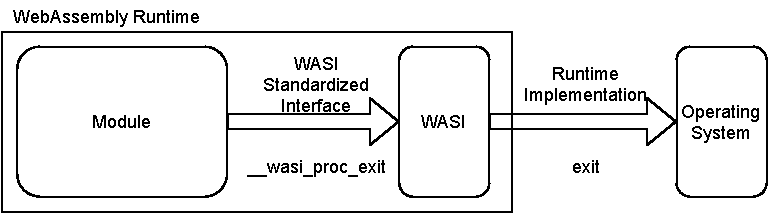
\includegraphics{Images/wasi-intro.pdf}
  \caption{A illustration of WASI}
  \label{fig:wasi-intro}
\end{figure}

\paragraph{WASI ABI model}
WASI classifies modules into two categories, command and reactors. A command
module has a single entry function, namely \texttt{\_start} and all the other
exported functions are not accessible by the user. On the other hand, reactor
modules have an optional initialization function named \texttt{\_initialize}.
If such initialization function is present, the runtime environment is obligated
to invoke such a function before calling others. The runtime environment may
invoke either the start or initializer function once during a module's lifetime.
Additionally, every WASI-compatible model needs to export a linear memory under
the name \texttt{\_memory}, and all addresses referred by modules are offsets
within such linear memory. Similarly, modules will also export an indirect table
with the name \texttt{\_\_indirect\_function\_table}. The runtime environment
will pass function pointers through the indirect table. Additionally, WASI
requires the runtime environment to provide all WASI API under module name
\texttt{wasi\_snapshot\_preview1} \footnote{This will change in the future, as
  WASI is still in the standardization phase.}.

\paragraph{Sandbox}
As we described above, WASI API follows WebAssembly's design philosophy, safety,
performance, portability, and compactness. WASI modules execute under a
capability-based security system to ensure the safety of the host environment.
The host runtime system will provide a sandboxed environment for each model. For
example, for file system access, WASI standard library C creates a virtual file
system for each module with the help of libpreopen \footnote{libpreopen:
  \url{https://github.com/musec/libpreopen}} \footnote{In the more recent
  version of WASI libc, libpreopen is no longer required.}.

\paragraph{Non-invasive and extensible}
In our discussion above, one may notice that a WASI-compatible module is also a
valid WebAssembly module on its own. WASI does not introduce new instruction nor
sections to the module; instead, it provides all additional functionality
through imported external functions. The design of WASI is also highly
extensible and split into separate modules. Currently, the WASI group focuses
on developing the core part that provides most of the POSIX interface, but it
may add additional features in the future.

\section{LLVM Compiler Infrastructure}

In the last section of this chapter, we would like to have a quick overview of
the compiler pipeline design and LLVM compilation framework. Designing a robust
and efficient in terms of both generated code and compilation speed compiler is
challenging. The LLVM compiler framework \cite{llvm-thesis} alleviates the
problem by introducing a standardized intermediate representation (IR) between
the compiler front end and its backend. Backend developers can target their
analysis and transformations on the IR instead of specializing in different
languages. On the other hand, frontend developers can translate the source
language into the IR and expect the backend to support multiple target platforms
with efficient code generation. Figure~\ref{fig:llvm-intro} illustrates the LLVM
compilation pipeline. In this project, we are interested more in the frontend of
the framework. The LLVM official documentation and tutorial provide full detail
of their intermediate representation \footnote{LLVM Language Reference Manual:
  \url{https://llvm.org/docs/LangRef.html}}. Here we will only discuss several
major differences between LLVM IR and WebAssembly that help understand the
thesis. We also provide an implementation of Adler-32 hashing in LLVM IR
generated with Clang in figure~\ref{fig:adler-32-llvm}.

\begin{figure}
  \centering
  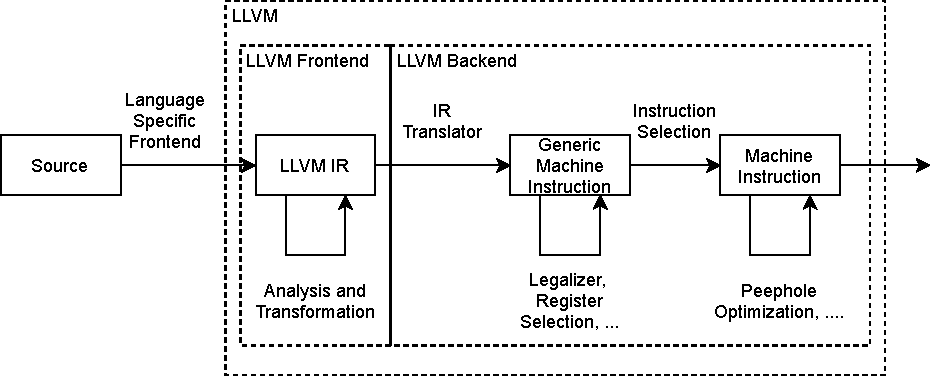
\includegraphics{Images/llvm-intro.pdf}
  \caption{A illustration of LLVM compilation pipeline}
  \label{fig:llvm-intro}
\end{figure}

\begin{figure}
  \centering
  \lstinputlisting[
    language=LLVM,
    basicstyle=\linespread{0.8}\small\ttfamily,
    numbers=left
  ]{Code/adler32.ll}
  \caption{Adler 32 in LLVM}
  \label{fig:adler-32-llvm}
\end{figure}

\paragraph{Register-based IR against stack-based IR}
In WebAssembly, all instructions operate over an implicitly declared stack. For
example, in figure~\ref{fig:adler-32-webassembly} at line $20$, a 32-bit integer
constant instruction, \texttt{i32.const}, will push the constant value on the
stack, and a 32-bit add instruction, \texttt{i32.add} will pop two values off
the stack as left-hand-side and right-hand-side operands accordingly, then push
the sum onto the stack. On the other hand, LLVM utilizes a register-based IR,
which is more similar to what one would expect on a native machine. In
figure~\ref{fig:adler-32-llvm}, each value for example, \texttt{\%0},
\texttt{\%1}, etc is a virtual register. Later in the backend, the register
allocation pass will map the virtual registers into physical registers using
register allocation algorithms.

\paragraph{Control flow, basic block, and $\phi$ instruction}
As we saw in previous sections, WebAssembly has specialized instructions to
manage the program's control flow. On the other hand, LLVM took a more
traditional approach to the problem. In 1991, researchers from IBM introduced
\emph{static single assignment} (SSA) form to ease the difficulty of writing
program analysis and transform passes \cite{ibm-ssa}. In SSA, each value has its
definition exactly once, and hence, the use-define chain (UD chain) is trivial
to compute. The UD chain presents the relationship between variable declarations
and variable-uses in a graph. It helps the analysis pass to efficiently pinpoint
the information about variables and identify if the variable declaration is
necessary or not. However, in most of the programs, these information needs to
be merged from different control-flows; for example, in a for-loop, the loop
counter may be defined in the initialization and on each loop iteration. The SSA
introduces a special kind of instructions, $\phi$ instructions, which mark the
explicit merge of definitions from different execution paths. LLVM adopts this
design principle in its intermediate representation. In
figure~\ref{fig:adler-32-llvm} we have multiple $\phi$ instructions. For
example, at line $11$ and $12$, value $\%7$ and $\%8$ represent $a$ and $b$
accordingly. We know that $a$ and $b$ initialized to $0$ and $1$ upon entry and
updated in each iteration from our C implementation. In the generated LLVM IR,
this merge induces $\phi$ instructions. For $a$ ($\%7$), if the control flow is
from the beginning of the function, we set its value to $1$, and on the other
hand, if the control flow is from the iteration, we update its value
accordingly. The different paths inducing a $\phi$ instructions are indicated by
basic block numbers. A basic block groups the maximum number of instructions
without control flow transfer. At line 11, we see the $\phi$ instruction merges
the definition coming from the $\%2$ which is the entry block and $\%4$.
Additionally, $\phi$ instructions must appear before any other instructions
within the same basic block. Additionally, $\phi$ instructions must appear
before any other instructions within the same basic block, as they model the
merging of values and do not have any execution semantics.

\paragraph{Memory and load-store instruction}
The last significant difference between WebAssembly and LLVM IR is on memory and
its related instructions. As we discussed earlier, a WebAssembly module can have
access to multiple linear memories \footnote{In the current version of
  WebAssembly, only one linear memory is allowed per module}. One might confuse
WebAssembly's linear memory with the concept of address space in LLVM IR. LLVM
IR associates each address with an integer value, namely, the address space.
However, unlike linear memory in WebAssembly, which has no difference between
one and another, the LLVM backend interprets the address space differently for
various architecture. For example, in the PTX backend, a backend target for
Nvidia GPUs, the implicit address space $0$ refers to traditional main RAM, and
address space $4$ represents the address shared by both main RAM and GPU RAM
\footnote{An introduction for PTX backend:
  \\\url{https://llvm.org/devmtg/2011-11/Holewinski_PTXBackend.pdf}}. For most of
the architecture, the implicit address space is the only address space available
to the programmer. Another difference between WebAssembly and LLVM IR is on
load-store instruction design. Load store instructions in both languages have an
attribute of alignment. However, LLVM IR interprets this attribute differently
from WebAssembly. In WebAssembly, the alignment attribute acts as a hint to the
runtime environment. If the alignment hint is unsuitable, the runtime
environment should still proceed under a possible penalty in the performance.
However, in LLVM IR, the alignment attribute is a requirement. Any memory access
that violates the alignment attribute will result in undefined behaviour,
usually a runtime panic. A load-store instruction in LLVM IR with alignment set
to one will never fail. However, it will be significantly less efficient as the
backend will likely generate byte-wise load and concatenation instructions.

We visited some of the background information that helps with understanding the
thesis in this chapter. In the next chapter, we will start from the beginning of
the system implementation, the WebAssembly parsing and validation frontend.
\chapter{Frontend}

This chapter describes the frontend of SableWasm. The front end consists of two parts, the bytecode parser and validation pass.  WebAssembly is a continuously evolving language, and its community might add new instructions in the future. Hence, the parser and the bytecode validation phase's design closely follow WebAssembly's specification and modular to ensure the framework's extensibility. A read-only view of the module structure provides additional functionality. The parser and validation phase design focuses on performance, both in execution time and memory footprint. 

\section{Bytecode Parser}
One of WebAssembly's binary format design goals is simple to parse. Although there are existing open-source bytecode parsing and validation library available when writing the thesis, such as WABT \footnote{WebAssembly Binary Toolkit: \url{https://github.com/WebAssembly/wabt.git}} provided by the WebAssembly community, there is no suitable library at the time when the project starts. Thus, for SableWasm, we implement our bytecode parsing frontend instead. The bytecode parser consists of three components, byte-source reader, WebAssembly bytecode parser and parser delegate. This section will give a brief description of each component, and figure~\ref{fig:sablewasm-parser} presents a general illustration of the parser's design.  

\begin{figure}
  \centering
  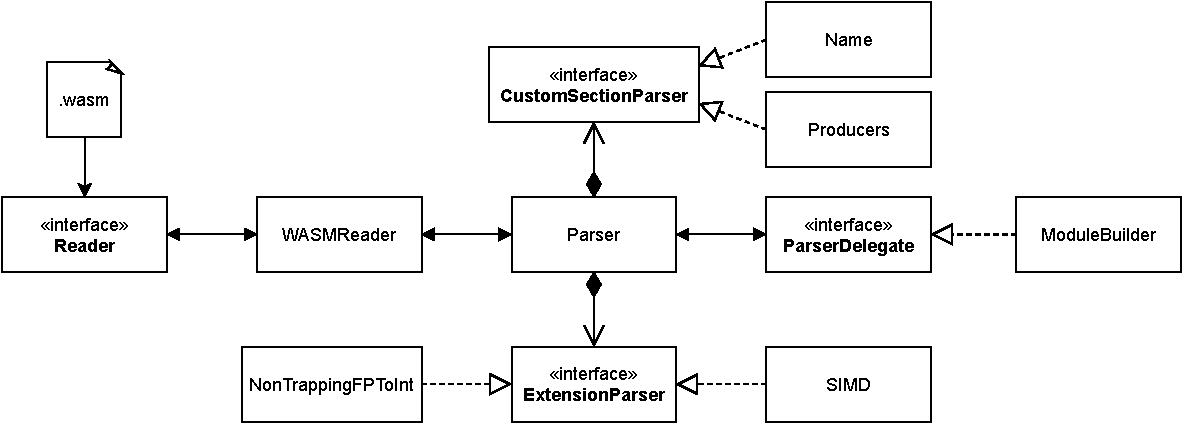
\includegraphics[width=\textwidth]{Images/sablewasm-parser.pdf}
  \caption{A illustration of SableWasm parser}
  \label{fig:sablewasm-parser}
\end{figure}

\paragraph{Byte-source Reader}
The byte-source reader consists of two parts, a byte-buffer reader and a WebAssmebly reader. The byte-buffer reader provides essential functionalities such as read and skips. Additionally, the byte-buffer reader also needs to support rewind and barrier. Any out of bound access, either beyond the barrier or byte stream exhausted, the byte-buffer reader will signal via exceptions. On the other hand, the WebAssembly reader provides a richer interface to the parser, such as decode LEB-128 encoded integers and parsing WebAssembly value types. The WebAssembly reader is also responsible for validating the result before passing it to the parser. In the case the result is invalid, the reader throws exceptions similar to the byte-buffer reader.

\paragraph{WebAssembly Parser}
WebAssembly parser is the kernel part of the parsing framework. As we discussed earlier in the chapter, one of the primary design goals of the framework is its extensibility. Hence, the SableWasm parser is modular and consists of three parts, parser core, custom section parser and instruction extension parser. The grammar for WebAssembly binary representation is quite simple, and therefore, the parser core implements a simple top-down recursive descent parser with a single byte look-ahead.

\emph{Custom sections} are a special section defined in the WebAssembly standard. They are essentially a binary data chunk tagged with a string name. How to interpret the binary data is different from one to another. These custom sections can either be standardized by the community or defined specific to a toolchain. In this project, we implement two custom sections standardized by the WebAssembly working group, namely \emph{Name} section and \emph{Producer} section. The \emph{Name} section gives human-readable names to functions and their local variables that help program debugging. The specification does not require these names to be the same as the import or export names. There is no direct support for more detailed debug information encoding in WebAssembly, at the time of thesis writing. However, extensions are working on this problem, such as DWARF for WebAssembly \footnote{DWARF for WebAssembly: \url{https://yurydelendik.github.io/webassembly-dwarf/}}; on the other hand, the \emph{Producer} section is relatively simple. It only encodes the information about the toolchain that generates the module, such as the toolchain name and version. All custom section parsers in SableWasm derived from the base class \texttt{CustomSection}. The parser core will dispatch the binary chunk to search custom section parser based on the name tag. Each custom section parser manages its results and does not communicate to the parser delegate directly. 

Instruction extension parsers focus on another different aspect of the WebAssembly module. In the background section, we have visited several extensions that merged to the WebAssembly specification. A quick reminder, WebAssembly extensions can insert or modify the instructions defined in the minimum-viable-product (MVP)  specification. The SableWasm WebAssembly parser employs instruction extension parsers to address this problem. When the parser intends to parse an instruction, it will iterate over all its instruction extension parsers in a chained manner. If the instruction opcode is not recognized by any registered instruction extension parser nor in the minimum-viable-product specification, the parser will signal the error by throwing an exception. An instruction extension parser can also override the default behaviour for MVP instructions by handling the instruction early, though, in the current version of WebAssembly, no extensions modify the semantics of these instructions. In this project, we implement two instruction extension parsers, the Non-trapping-float-to-int conversion parser and SIMD parser, which handles the instructions introduced by the extensions as their names suggest.

\paragraph{Parser Delegate} The last part of the SableWasm WebAssembly bytecode parser is the parser delegate. The parser delegate and parser are direct implementations of the common delegation patterns seen in many other projects, separating the parsing from the heavy lifting of module construction. One can implement a validation pass at this level without module construction. However, in this project, we implement our bytecode validation pass after the module construction, giving space for further projects focusing on bytecode-level transformation. We will discuss the implementation of such validation pass later in the chapter. 

In this section, we give a brief overview of the parser framework introduced in the SableWasm. In the next section, we will discuss the WebAssembly bytecode representation used in the project and several techniques to improve the performance and ensure flexibility.

\section{WebAssembly Bytecode Representation}

\begin{figure}
  \centering
  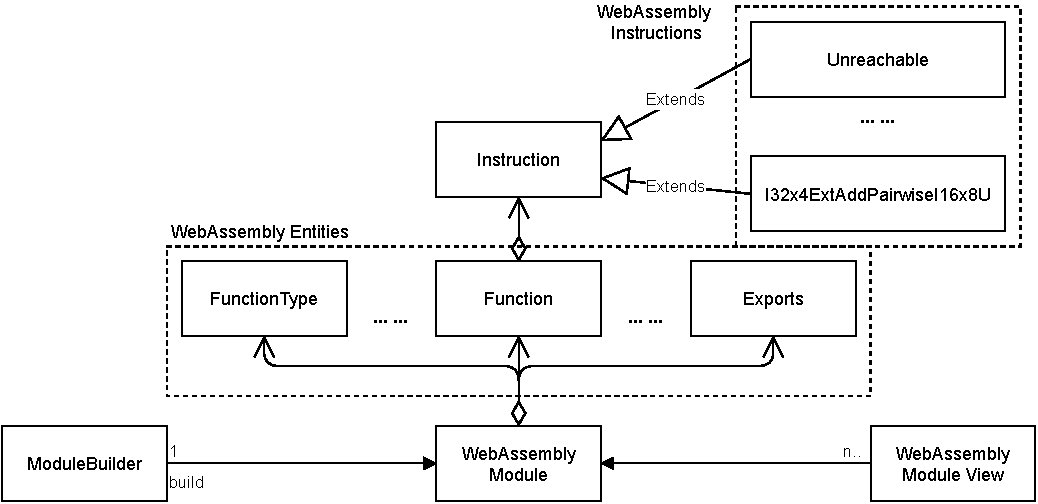
\includegraphics[width=\textwidth]{Images/sablewasm-bytecode.pdf}
  \caption{A illustration of SableWasm Bytecode Representation}
  \label{fig:sablewasm-bytecode}
\end{figure}

WebAssembly specification provides a compact and representation in both binary format, and text format \cite{10.1145/3062341.3062363}, and these specifications might subject to change in the future. In SableWasm, we implement our bytecode representation as close to the specification as possible.  Hence, in the future, if the community alters the specification in the future, we can apply fixes to the bytecode representation in a straightforward manner without introducing extra complexity. In figure~\ref{fig:sablewasm-bytecode}, we present an illustration of the bytecode representation used in SableWasm. Compare to the representation given in the WebAssembly specification, the only difference we have is the function section. The standard WebAssembly bytecode representation actually splits the function section into two different sections, namely \emph{function} and \emph{code}, to achieve its one-pass validation goal. The \emph{function} section contains the type of all functions defined in the module, serving similar to function declarations in other languages. Later in the module, \emph{code} section defines them. On the other hand, in SableWasm, we merge these two sections into a single function section. A function in SableWasm bytecode representation contains both its type and its definition.

\paragraph{WebAssmebly Module View} The WebAssembly module structure only serves as a storage container for the bytecode representation and itself does not provide an interface to the user, except retrieving entities by index. Additionally, WebAssembly standard binary format focuses more on compactness instead of usability, which leads to complexity when retrieving the information. For example, to avoid duplication, the function types are stored in their section, namely, \emph{type} section. Later in the module, any reference to the type becomes an indices respect to this section. Another example is entity indices. WebAssembly specification requires that every import entry in the \emph{import} section implicitly introduces an index in its corresponding class. These indices should come before any definition introduced in the module. These two rules suggest that to retrieve an entity by index, one should first iterate over all the imports and then locate the entity accordingly, which is a relatively expansive operation. To address these problems, we implement a read-only view of the WebAssembly module that cache the indices and provides additional features. 

\paragraph{Instructions} SableWasm takes a traditional `abstract syntax tree' approach to bytecode instruction representation. The frontend represents each instruction using a corresponding class derived from a common base class, namely \texttt{Instruction}, and an expression with a vector of instruction pointers. One observation is that the heap memory usage grows linearly respective to the size of the expression, which is not optimal. In WebAssembly, instructions operate over an implicitly defined stack, and for most of the operation, there is no operand attach to them. For example, \texttt{F32x4Nearest} has no operand, and it will pop a value from the stack, treat it as a vector of packed single-precision floating-point values, round them to the nearest integer, finally push the result back to the stack. From the bytecode representation point of view, there is no difference between one instruction without operand and another with the same opcode. Hence, to reduce memory consumption, we use pointers that point to object singleton to represent instruction without operand. However, how can we distinguish a pointer points to an object from one referring to a heap-allocated object which requires memory deallocation? To address this problem, we use tagged pointers. For a non-heap allocated singleton object, we tag the least significant bit in the pointer with zero; and on the other hand, we tag that of a heap-allocated object pointer with one. Later, within the destructor, we only need to exam the least significant bit of the pointer and perform memory de-allocated in the case when needed. With tagged pointer techniques, we can greatly reduce the memory needed to store the bytecode representations while maintaining their polymorphic nature. As less memory allocation is needed, we also observe performance improvement in terms of execution time, which we will later see in this chapter.

This section gives an overview of the bytecode representation used in SableWasm and several techniques to improve its performance. In the next section, we will move to the validation pass implementation in SableWasm.

\section{WebAssembly Bytecode Validation}

WebAssembly specification defines a  detailed validation rule both for well-formedness, and type-soundness \cite{10.1145/3167082}. Similar to the parser framework, we implement our validation pass as close to the specification as possible. If there are changes to the specification in the future, we can adopt them with minimal effort. The validation pass implementation consists of two parts, the validation context and validation visitor, implementing context and rules in the specification accordingly. 

\section{Performance Evaluation}

adsfadsf
\chapter{Middle-level Intermediate Representation}

This chapter describes SableWasm's middle-level intermediate representation (MIR), which has a critical role in the entire compilation pipeline. MIR acts as a middle ground between the WebAssembly bytecode frontend and various possible backend. SableWasm only implements one backend that currently utilizes the LLVM compilation framework, but adding more backend support should not require significant modification on the MIR. It also implements an analysis and transformation framework where we perform several optimizations over the MIR. We will first go over the overall design of the MIR, then later move to the translation strategy we used to translate WebAssembly bytecode to MIR. Finally, we will end the chapter with several analyses and transformations we implemented.

\section{MIR Design}

In the previous chapters, we have quickly covered the design of WebAssembly bytecode. A quick reminder, WebAssembly is a stack-based intermediate representation (IR) where all instructions operate over an implicitly declared operand stack. There are several advantages of stack-based IR. Perhaps the most important one is its portability. A stack-based IR makes fewer assumptions on the machine than a register-based one.  One can even provide an implementation for a hypothetical machine with only one register. Another advantage is the code size. Experiments show that, in general, stack-based IR is relatively more minor in size than its corresponding registered version \cite{stack-and-register-vm}. When designing a binary format that ships executables over the internet, the stack-based IR seems to be a better choice for WebAssembly.

Nevertheless, there are no silver bullets; stack-based IR design has its drawbacks. One of them is the difficulty when performing code analysis and transformation over the module. As for each instruction, its operands implicitly come from the stack; the value use-def relationship between instructions is not apparent to the analysis, and recover such connection between instructions from the IR is not a trivial task.

\begin{figure}
  \centering
  \lstinputlisting[language=SableWasmMIR, basicstyle=\small, numbers=left]
  {Code/4.MIR/fibonacci.mir}
  \caption{Fibonacci in translated SableWasm MIR}
  \label{fig:mir-fibonacci}
\end{figure}

On the other hand, we have the register-based intermediate representation, more specifically, the infinite-register machine. The infinite-register machine is similar to what one would expect from an actual physical machine. The only difference that the infinite-register machine, as the name suggests, has an infinite amount of registers. For each instruction in register-based IR, it has its operand encoded in the instruction. Hence, the use-definition relationship will become explicit to the analysis and transformation. The main design goal for SableWasm MIR is to provide an analysis platform for the entire compiler system. Thus, we implement our MIR as an infinite register machine. We also take a traditional approach in various other aspects. For example, instead of using the structured control flow similar to what WebAssembly offers, we use control-flow graphs (CFGs) to represent the relationship between basic blocks. The SableWasm MIR is also in single static assign (SSA) form \cite{ibm-ssa}, covered in the background chapter. The design for instruction and module-level entities in SableWasm MIR is quite similar to what WebAssembly instruction offers. One can view the SableWasm MIR as a mixture of LLVM intermediate representation and WebAssembly bytecode. We also adopt several design features from LLVM IR into MIR, such as use site lists. In SableWasm MIR, all elements are derived from the base class \texttt{ASTNode} which offers the implementation to these features. The base class automatically manages the use sites list, which is helpful later in MIR analysis and transformation.

Figure~\ref{fig:mir-fibonacci} shows a simple function that calculates Fibonacci numbers with a recursive method in SableWasm. With the help of the figure, we will go through the detailed design of SableWasm later in the chapter. We will first present the module-level entity design and their initializer expressions, such as functions, then move to the design of each instruction defined in MIR.

\subsection{MIR Initializer Expressions}

\begin{figure}
  \centering
  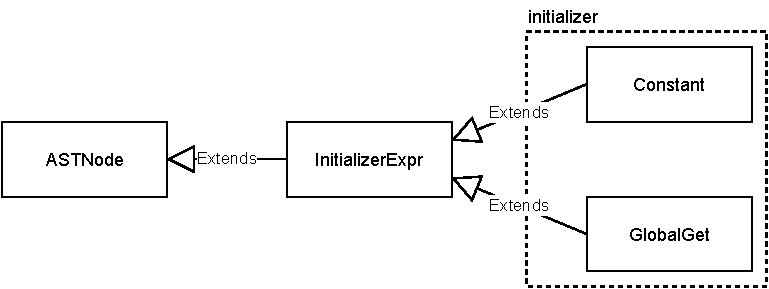
\includegraphics[width=\textwidth]{Images/4.MIR/initalizer-expression.pdf}
  \caption{SableWasm MIR Initializer Expression}
  \label{fig:sablewasm-mir-initializer-expression}
\end{figure}
   
WebAssembly defines a particular form of expression, namely constant expressions. They can appear in three locations in the current specification. First, global variables declaration can contain constant expression as their initialization values. Additionally, data section entries and element section entries can have constant expressions as the offsets for their initialization payload. In SableWasm MIR, we define initializer expressions that act similar to what constant expression does in WebAssembly. Figure~\ref{fig:sablewasm-mir-initializer-expression} gives a general illustration about SableWasm MIR initializer expressions. The initializer expressions are quite simple. In the current WebAssembly and SableWasm, an initializer expression can be either a constant value or refer to an imported global via \texttt{GlobalGet} instruction. Hence, in principle, currently, SableWasm MIR initializer expression is essentially a single instruction. In the future, one may generalize such constrain by allowing more complex constructs in initializer expressions. 

\paragraph{Constant}
The \texttt{Constant} instruction represents a single constant value for the initializer expression. In WebAssembly, a constant value can be one of the following: a 32-bit or 64-bit integer, a floating-pointer number or a 128-bit SIMD vector \footnote{with WebAssembly SIMD128 extension}, and the specification encodes type within the instruction opcode. Hence, there are multiple instructions in WebAssembly to introduce a constant. In SableWasm, we do not encode the type into the opcode, and \texttt{Constant} instruction is the only instruction that takes care of the task. In figure~\ref{fig:sablewasm-mir-initializer-expression}, we have a constant initializer at line 6 that initializes the values of the global to a 32-bit integer with a value that equals 66560. When querying the type of a \texttt{Constant} instruction, SableWasm will infer it from its payload constant.

\paragraph{GlobalGet}
The \texttt{GlobalGet} instruction is exactly same as the WebAssembly's \texttt{global.get} in execution semantics. WebAssembly specification allows any initializer refers to an imported \footnote{This might subject to change in the future version of WebAssembly} global value. As these values are initialized before the module, reading the value from them is always valid during module initialization. The example in the figure does not provide an example of \texttt{GlobalGet} as an initializer expression. They are less frequently used compare to constant initializer expression, especially for global values. However, in some ABI implementations, data section entries and element section entries require to read from global values serving as base pointers. SableWasm also infer the type for \texttt{GlobalGet} initializer expression in a similar fashion as \texttt{Constant}. In this case, the type of instruction is the same as the referred global variable without the constness modifier.

In this section, we cover the design and implementation of initializer expressions in SableWasm. They are pretty simple in the current design. We will now move to the next part in the SableWasm design, the module-level entities.
\subsection{MIR Module Entities}

\begin{figure}
  \centering
  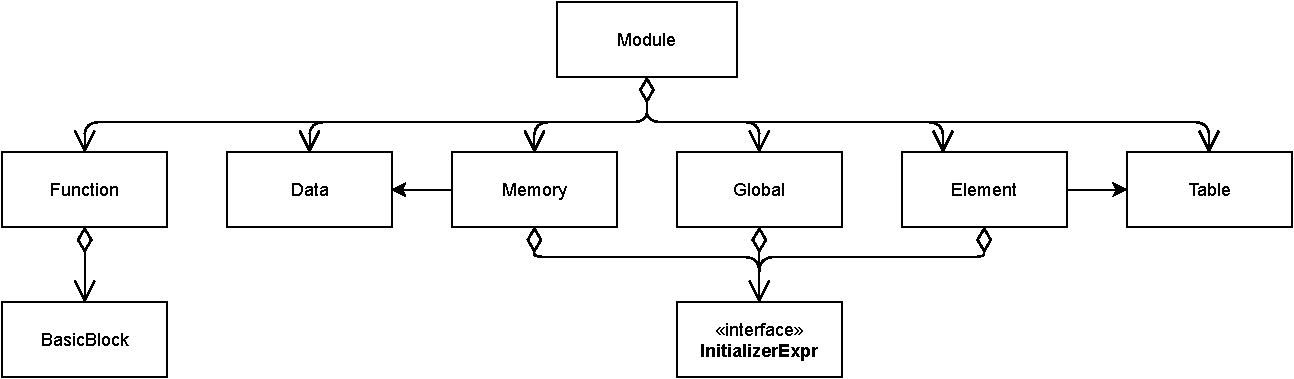
\includegraphics[width=\textwidth]{Images/4.MIR/module.pdf}
  \caption{SableWasm MIR Module-level entities}
  \label{fig:sablewasm-mir-module}
\end{figure}

SableWasm module-level entities are the top-level elements in a translation module. They are direct implements of the WebAssembly module entities defined in the specification. Figure~\ref{fig:sablewasm-mir-module} presents a general illustration of the SableWasm module-level entities. In this section, we will cover the design of each entity and compare them with its WebAssembly correspondent.

\paragraph{Function}
In figure~\ref{fig:mir-fibonacci}, we have a function definition at line 8. A function declaration in SableWasm provides information about the type, local variables and name. A function definition should satisfy all the requirements of function declaration, and additionally, provides a function body using basic blocks. The design of the function declaration and definition in SableWasm is quite similar to that of WebAssembly. The major difference is how to represent the function body. We will come back to this in the later sections within the chapter. Finally, like other module-level entities, a SableWasm function can optionally have import or export annotations. These annotations provide names for the import and export entries in the WebAssembly module.

\paragraph{Global}
SableWasm's global variable declaration and definition follow the design in WebAssembly. In SableWasm, we relax several of the constrain defined in WebAssembly specification and its extensions. In the SIMD extension proposal, the 128-bit vector type is only suitable within the function body. There is no direct way to pass a vector value to the host environment, as there is a lack of standard representation for 128-bit packed vectors in JavaScript \footnote{This might subject to change in the future. WebAssembly SIMD extension proposal is still in the drafting process.}. In  SableWasm, we treat all primitive types uniformly. Thus, a global variable can contain an integral value, a floating-point value or even a packed SIMD vector. The type for the global variable follows the specification in WebAssembly; it is a pair of value type and constness modifier. In figure~\ref{fig:mir-fibonacci}, we have a global definition at line 6, which contains a mutable 32-bit integral value. All global variable definitions in SableWasm must provide a value initialization via initializer expression, which we covered in the previous section. The rules for import and export annotation on the SableWasm function entities also apply to SableWasm global variables, which we do not show in the example above.

\paragraph{Memory and Data}
Memory and Data are implementation for WebAssembly linear memory and its initializer, respectively. One might think that there is no need to separate the memory initializer from the memory entity definition, as in WebAssembly specification, all data section entries must provide a valid linear memory index. In the early version of SableWasm, we indeed adopt such implementation. However, this approach might be subject to a significant change in an extension that might soon merge to the WebAssembly specification. The WebAssembly bulk memory operation extension proposal \footnote{WebAssembly bulk memory operations: \\\url{https://github.com/WebAssembly/bulk-memory-operations}} introduce new instructions, such as \texttt{memory.fill} that direct refers to a data section segment. Moreover, the proposal relaxes the constrain on the linear memory index. Now the index can behave like a flag indicating whether the data segment itself is active or not and no longer serves as a linear memory index. Hence, to make our framework `futureproof', we separate the linear memory declaration from their initializers. Figure~\ref{fig:mir-fibonacci} presents a linear memory definition at line 2. SableWasm memory entities also adopt WebAssembly linear memory type. The type consists of a pair of unsigned integers, indicating the lower bound and upper bound of the memory size in WebAssembly pages. Finally, the memory entity can have import and export annotations similar to other module-level entities in SableWasm. The example above defines a memory with a minimal size of 2 pages, 128KiB, and exports it under `memory'. The example above does not provide any example for data initializers, but they are quite easy to understand. A data initializer is essentially a binary chunk with an initialization offset. They are semantically equivalent to a data section entry in an ELF file.

\paragraph{Table and Element} SableWasm table and element entity implements the indirect table and its initializer, namely element segment, accordingly. They follow the simple principle as the memory and data entity in the previous section. Currently, like data segment entry, WebAssembly's element section entry must refer to a valid indirect table via an index. In the future, this may also subject to change. WebAssembly reference types extension proposal \footnote{WebAssembly reference types: \url{https://github.com/WebAssembly/reference-types}} introduce instructions such as \texttt{table.fill} that are able to have direct access to element segment initializers. \texttt{table.fill} instruction is similar to \texttt{memory.fill} defined in the bulk memory operation extension. It will copy a sequence of compile-time defined function pointers into an indirect table at runtime. Thus, when we design our table entity, we also split the declarations from their initializers. The type for table entity is the same as the table type in WebAssembly. It consists of a pair of unsigned integers, indicating the lower bound and upper bound for the number of function pointers stored in the indirect table. In SabelWasm MIR, we treat memory entities and table entities as black boxes, and its concrete implementation is deferred to the backend. The example shown in figure~\ref{fig:mir-fibonacci}, the module defines a table entity at line 4 that stores exactly one function pointers. Note that the table entity does not require users to initialize the value for all entries. The table entity default initializes all entries to null pointers. Finally, the rule for import and export annotation also apply for table entity. However, the element entity is local to the module and can neither export nor import from other modules.

In this section, we cover the design for module-level entities in SableWasm. They are pretty similar to the sections defined in WebAssembly specification. In the next section, we will move the design of SableWasm instructions.
\section{MIR Instructions}

SableWasm MIR uses a control-flow-graph (CFG) based representation in
\emph{static single assignment} (SSA) form to represent code body in function
definitions. We have provided an introduction to CFG and SSA in the background
chapter. Here is a quick recap. CFG splits the control flow within the function
into basic blocks. A basic block represents the most extended instruction
sequence without control flow transfer, such as branching. Note that for
function calls, we take a similar approach to that of LLVM. We will come back
to this in detail later in this section. Additionally, SSA requires that all
values must have unique definition sites. Hence, in SSA form, the
use-definition chain is trivial to compute, while in a traditional CFG, one
would need to extract this from the graph with the help of a \emph{reaching
  definition} analysis. The SableWasm MIR instruction set is similar to
WebAssembly bytecode in terms of semantics for most of the instructions.
However, it operates over an infinite register machine instead of a
stack-based machine, and in some cases, semantics differ in order to keep the
size of the SableWasm instruction minimal. In this section, we will cover the
design and implementation of SableWasm MIR instructions. The following section
will cover the translation strategy between WebAssembly bytecode and the
SableWasm MIR and instruction reduction rules.
Figure~\ref{fig:sablewasm-mir-inst} provides a general illustration of the
design of the SableWasm MIR instruction set. The SableWasm MIR instruction set
can currently cover all the instructions defined in WebAssembly specification,
including several extensions such as multivalue and SIMD vector operations.

\begin{figure}
  \centering
  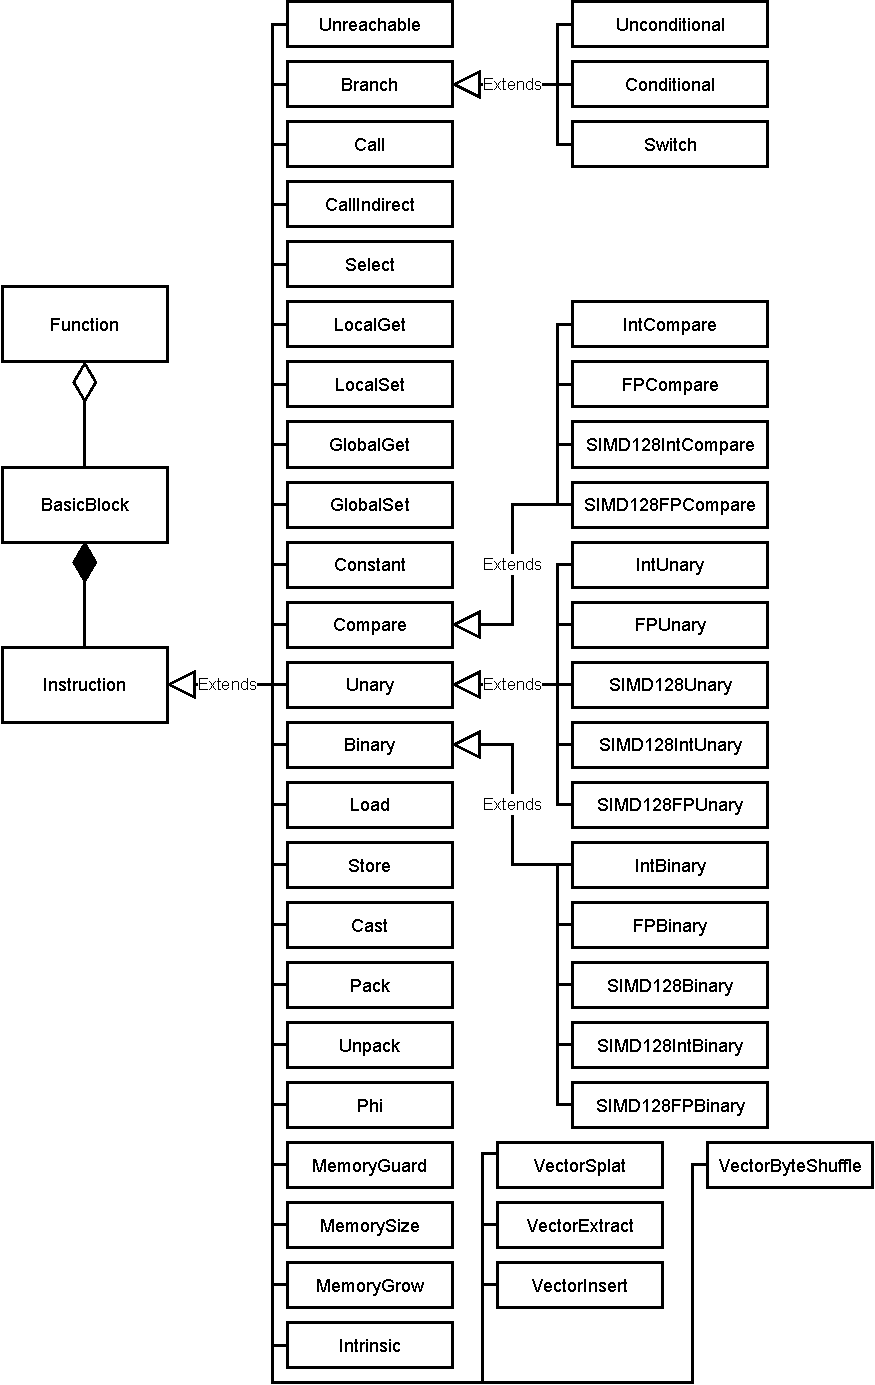
\includegraphics[width=0.8\textwidth]{Images/4.MIR/sablewasm-instruction.pdf}
  \caption{SableWasm MIR Instructions}
  \label{fig:sablewasm-mir-inst}
\end{figure}

\paragraph{Terminating instructions}
As discussed above, SableWasm splits the function control flow into basic
blocks containing the maximum number of consecutive instructions without
control flow transfer. In addition, SableWasm, similar to many other SSA form
instruction sets, defines a particular group of instructions called terminating
instructions. These instructions signal a control flow transfer out of the
current basic block, and they must only appear as the last instruction in any
given basic block. SableWasm defines four different terminating instructions:
unreachable, unconditional branching, conditional branching, and table
branching. If the control flow reaches a \texttt{Unreachable} instruction,
the runtime system will signal a runtime panic. The \texttt{Unreachable}
instruction in SableWasm is identical to its counterpart in WebAssembly in
terms of semantics. The \texttt{Unconditional} instruction is an unconditional
control flow transfer, as the name suggests. It refers to a target basic block
as the operand. At runtime, the instruction will always transfer the control
flow to the target basic block. \texttt{Unconditional} is similar to the
\texttt{br} instruction defined in WebAssembly specification. On the other hand,
\texttt{Conditional} is a conditional branching. It takes a value and two
target basic blocks as its operands. At runtime, the instruction will first
compare the value against integral value zero. If the value equals zero, the
instruction will transfer the control flow to the `false' basic block,
otherwise, to the `true' basic block. SableWasm's \texttt{Conditional}
instruction is similar to \texttt{br.cond} defined in WebAssembly. The last
terminating instruction defined in SableWasm is \texttt{Switch}.
\texttt{Switch} instruction is comparable to the \texttt{br.table} instruction
in WebAssembly. The instruction takes a value, a list of target basic blocks,
and a default branching basic block as its operands. At runtime,
\texttt{Switch} will interpret the value as an integral value and dispatch
accordingly. If the value is within the branching list's range, it will
redirect the control flow to the target basic block referred to by the index.
Otherwise, \texttt{Switch} will transfer the control flow to the default basic
block.

\paragraph{Function call}
In SableWasm, we provide two instructions for function calls defined in
WebAssembly specification: direct function calls and indirect function calls.
\texttt{Call} represents a direct function call where the callee is known at
compile time. It takes a function and a list of arguments as operands. On the
other hand, \texttt{CallIndirect} defines an indirect function call. It
implements the indirect function call protocol described in the WebAssembly
specification. A quick reminder, in WebAssembly, an indirect function call takes
an indirect table, the table index, the expecting function type, and a list of
values as arguments. At runtime, the system should first check if the index is
valid for the indirect table and fetch the function pointer and its actual
signature accordingly. Then, the system should compare the signature against the
expecting type. If the signature matches, the runtime system will
transfer the control flow to the function referred to by the function pointer.
Implementing the signature verification mechanism is backend-specific; we will
return to this topic in the next chapter. Note that we do not treat function
call instructions as terminating instructions, even though they transfer the
control flow to other locations. In SableWasm MIR, we follow the design like
that used in the LLVM intermediate representation, where it is assumed that
the control flow will continue to the next instruction after returning from the
function call. Hence, from the basic block's local perspective, their control
flow is pre-determined, and there is no difference compared to other
non-terminating instructions.

\paragraph{Local and global variable access}
In WebAssembly, instructions have access to locals defined by their parent
functions and global variables defined by their enclosing module. The SableWasm
MIR defines getter and setter instruction for both local and global variables to
implement the specification. Their semantics are the same compare to
WebAssembly's counterparts. We will skip the detail here, but one can consult
the WebAssembly specification for detailed information.

\paragraph{Numerical operations}
In SableWasm, we classify the numerical operations into three different
categories, the \texttt{Compare} instructions, \texttt{Unary} instructions, and
\texttt{Binary} instructions. The \texttt{Compare} instructions implement the
comparison between values, such as `equal to'. They always yield a 32-bit
integer as WebAssembly specification suggests. The \texttt{Unary} and
\texttt{Binary}, as their name suggests, perform unary and binary operations
between values. The result of \texttt{Unary} and \texttt{Binary} instruction is
dependent on the opcode. On the other hand, we can also orthogonally classify
the instructions into integer, floating-point, packed integer, and packed
floating-point numbers. Note that in MVP WebAssembly, there are only integer and
floating-point value operations; the SIMD operation extension proposal adds the
packed value operation to the instruction set. In the WebAssembly SIMD extension
proposal, the vector value does not store its size and content information in
the types. Instead, the packed value instructions' opcodes keep track of the
shape of the vector values, which leads to the bloated instruction opcodes. In
SableWasm, we separate the instruction opcode from the vector shape. For each of
the packed value operations, it must have either a \texttt{SIMD128IntLaneInfo}
or \texttt{SIMD128FPLaneInfo}. Figure~\ref{fig:sablewasm-mir-inst} shows all the
classes of numerical operations defined in SableWasm. For detailed opcodes in
each numerical instruction class, one can consult SableWasm's source code.

\paragraph{Load and Store}
\texttt{Load} and \texttt{Store} instruction provides access to the linear
memory for SableWasm MIR. Although in the current version of WebAssembly, the
module can contain at most one linear memory, and all WebAssembly's load and
store instructions implicitly refer to this linear memory \footnote{This might
  change in the future version of WebAssembly.}. In SableWasm MIR, we take a
different approach. The SableWasm MIR's \texttt{Load} instruction takes a linear
memory and an integer value as operands. At runtime, the value will be treated
as the address (or offset) to the start of the linear memory, and the
instruction yields the fetched result. In WebAssembly, the \texttt{load}
instruction associates with a type and an extension method. For example,
\texttt{i32.load8\_s} loads an 8-bit integer from the linear memory, and then
sign extends the fetched byte into a 32-bit integer. In SableWasm, the
\texttt{Load} instruction associates to a type and an integer value, namely the
load width. The load width must equal to or smaller than the width of the type.
Also, SableWasm \texttt{Load} always perform zero-extension on loaded value.
Hence, when translating WebAssembly's sign-extended load into SableWasm's
\texttt{Load}, one must combine the load instruction with a cast instruction.
We will come back to this in chapter~\ref{chapter:mir-translation-optimization}.
The \texttt{Store} instruction
also associate with a store width. Like the load width defined for \texttt{Load}
instruction, the store width must also be equal to smaller than the store value
type's width. The system will first bit truncate the value at runtime and then
store the result into the linear memory. One may notice that in SableWasm, we
erase the alignment attribute and offset attribute defined in WebAssembly.
Currently, we do not support alignment hints from the WebAssembly module. In
SableWasm, the \texttt{Load} and \texttt{Store} always have the alignment
requirement of one byte. This implies that the \texttt{Load} and \texttt{Store}
can happen anywhere in the linear memory, corresponding to WebAssembly's linear
memory specification.

\paragraph{Linear memory manipulation}
WebAssembly specification defines two instruction that works with linear
memories: \texttt{memory.size}, \texttt{memory.grow}. Like the WebAssembly's
\texttt{load} instruction we covered in the previous paragraph, all these
instructions operate over the implicitly defined unique linear memory within the
module. In SableWasm, we provide similar \texttt{MemoryGrow} and
\texttt{MemorySize} instruction. The semantics of SableWasm's memory
manipulation instructions are the same as their WebAssembly counterparts, except
that the linear memory needs to be explicitly stated. In SableWasm, we introduce
one additional instruction, \texttt{MemoryGuard} which is an explicit memory
boundary check. In WebAssembly, all \texttt{load} and \texttt{store} instruction
need to check for linear memory out of bound error before access. SableWasm
separates the bound check from the memory access. One advantage of this is that
one may implement static memory bounds check elimination optimization over
SableWasm MIR. Additionally, one backend may provide different strategies for
handling boundary checks, such as utilizing invalid virtual memory pages with
the operating system's help. In this case, we only need to modify the
translation pattern for \texttt{MemoryGuard}. \texttt{MemoryGuard} takes a
linear memory and an integer value as the operand. It also associates with an
integer immediate, known as the guard width. At runtime, the system will perform
a boundary check over the linear memory starting from the given address to
determine if it contains at least a given number of bytes ahead. If there are
not enough bytes available, the system should signal a runtime panic.

\paragraph{Pack and Unpack}
WebAssembly multivalue specification \footnote{WebAssembly Multi-value Proposal:
  \url{https://github.com/WebAssembly/multi-value}} relaxes the constrains on
the function type. Functions now can return multiple values instead of at most
one value. To support these features, we introduce \texttt{Pack} and
\texttt{Unpack} instructions, along with extending WebAssembly's type system.
\texttt{Pack} instructions group multiple values into a single ordered tuple,
while the \texttt{Unpack} reverse the operation by retrieving the value from
tuples by index. In the case where a function returns multiple values, we thus
use a tuple instead. SableWasm treats tuples as first-class values; however,
currently, tuples cannot be recursive. We will come back to this
in chapter~\ref{chapter:mir-translation-optimization},
when we visit the type systems of SableWasm MIR. The index of the
\texttt{Unpack} must be an immediate value in the current version of SableWasm
MIR and is verified at compile time.

\paragraph{Vector operations}
In the previous paragraph, we introduce the numeric operations defined in
SableWasm MIR. However, several instructions do not fit into either
\texttt{Unary} or \texttt{Binary} instructions. Hence, to faithfully support the
SIMD operations introduced by the extension proposal, we add four
vector-specific operations into SableWasm MIR. They are \texttt{VectorSplat},
\texttt{VectorExtract}, \texttt{VectorInsert} and \texttt{VectorByteShuffle}.
\texttt{VectorSplat} will broadcast the operand value to all lanes in the result
vector. SableWasm MIR defines vector splat operation for both packed integer
vector and packed floating-point vector. \texttt{VectorExtract} is similar to
the \texttt{extractelement} defined in LLVM intermediate representation. It
takes a vector as the operand and also associates itself with an immediate
integer value. At runtime, the system extracts the value of the given lane and
yields as a result. \texttt{VectorInsert} is similar to \texttt{insertelement}
defined in LLVM. It will replace the vector operand with a given value and
yields the updated vector as a result. Note that in the WebAssembly SIMD
extension proposal, there are more instructions defined that modify the
individual lane value of the vector, such as \texttt{V128Load32Lane} which
loads a 32-bit value into a specific lane within the vector. In this project,
we would like to keep our instruction set simple; hence, these instructions are
reduced into multiple SableWasm MIR instructions. We will come back to this
in chapter~\ref{chapter:mir-translation-optimization}
when we discuss the instruction reduction rules. The last
instruction we introduced is the \texttt{VectorByteShuffle}.
\texttt{VectorByteShuffle} is similar to \texttt{shufflevector} defined in LLVM,
except that it allows rearranging bytes instead of lanes. Currently, the
\texttt{VectorByteShuffle} only operates over an array of immediate integer
values. Compare to the lane shuffle semantics, byte shuffle semantics provides
more precise control over the result value. One can trivially simulate a lane
shuffle with a byte shuffle. The WebAssembly SIMD extension proposal only
defines shuffle for \texttt{i8x16}, which corresponding to the byte shuffle
semantics. However, in the future, if another shape vector supports shuffle
operation, one can generalize the implementation with minimal modification.

\paragraph{Cast}
\texttt{Cast} models the conversion of values to their equivalent form in other
types. In SableWasm MIR, we do not distinguish between value conversion and
value extension. We treat signed and zero extensions as a kind of value
conversion. The \texttt{Cast} instruction takes a single value as the operand,
and it associates itself with a cast opcode. At runtime, it will perform the
conversion according to the opcode, and if the result cannot be accurately
represented in the target type, the system should signal a runtime error.
The cast opcodes are direct implementations of their WebAssembly counterparts,
and we will skip the detail here. One may refer to the WebAssembly specification
for more details.

\paragraph{Intrinsic}
The last SableWasm MIR instruction we are going to cover in this section is the
\texttt{Intrinsic} instructions. Most WebAssembly instructions can be
represented by using the SableWasm MIR instructions, which we covered earlier in
this section. However, there are still several corner cases. For example, the
WebAssembly SIMD extension proposal defines Q-format rounding multiplication, a
type of fix-point multiplication, for packed 16-bit integers. Another example is
the \texttt{swizzle} operation. A \texttt{swizzle} operation is similar to a
shuffle operation, except that it takes another vector as the shuffle indices
vector instead of an array of immediate integer values. These operations are
only defined for a specific vector shape and will introduce unneeded complexity
to the SableWasm MIR if we generalize them to all possible vector shapes. Hence,
here we group these instructions as the \texttt{Intrinsic} instructions. There
is no direct mapping to LLVM instruction for most of them, even with the
intrinsic functions provided by the framework. Hence, the backend is encouraged
to support these instructions with runtime library routines.

In this section, we discussed the design of the SableWasm MIR instruction set,
and in the next chapter, we will move to the translation strategy between
WebAssembly and SableWasm MIR along with the analysis and transformation
framework.

\section{Translating WebAssembly to MIR}

In this section, we will cover the translation between WebAssembly bytecode and SableWasm MIR. We have covered the design of SableWasm MIR instructions previously. One may notice that for most of the instructions, especially for the numerical operations, SableWasm MIR shares the same semantics as WebAssembly. Hence, the translation rules for these instructions are pretty trivial, and we will not cover them in detail in this section. Instead, this section will focus on the translation rules for the structured control flow construct and WebAssembly instructions that require reduction during translation.

The translation framework is similar to the validation framework we discussed in the previous chapter except for two significant differences. First, the operation stack will keep track of the values generated during translation instead of types. Let's take \texttt{i32.add} as an example. \texttt{i32.add} instruction takes two values from the stack and then performs 32-bit integer addition between them. Finally, it will push the result type back onto the stack. In the case of translation stack, we pop two values from the stack and assume they are 32-bit integers. In SableWasm MIR, we use pointers to instructions to refer to the values generated by them. Then, the translation visitor will build a \texttt{IntBinaryOp} instruction, with \texttt{Add} as opcode, and two pointers as operands. Finally, the visitor will append the instruction to the current active basic block and push the instruction pointer of \texttt{IntBinaryOp} onto the stack. Another difference between the validation framework and the translation framework is the labels stack. In the validation framework, the labels stack stores the resulting types generated from the label. In the translation framework, the labels stack stores the potential landing basic blocks for the labels. We will revisit this with more details later in this section.

\subsection{Structured-Control-Flow Construct}

Translating from stack-based IR to register-based IR is not trivial, especially
when non-linear control flow structures appeared. This problem appeared in many
runtime system implementations, such as Numba \cite{numba}, a just-in-time (JIT)
compiler for Python. Usually, one needs some algorithm to recover the control
flow structure from annoying jump instructions. Luckily, in WebAssembly, we can
translate the stack-based bytecode into register-based basic blocks in linear
time, thanks to the structured control flow constructs and their validation
rules defined in WebAssembly. In this section, we will cover the translation
patterns used for WebAssembly's structured-control-flow constructs, namely
\texttt{block}, \texttt{if} and \texttt{loop}.

\begin{figure}
  \centering
  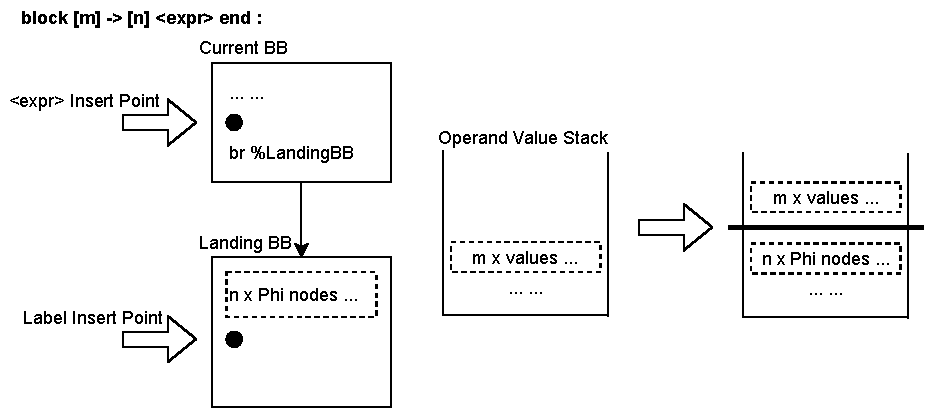
\includegraphics[width=\textwidth]{Images/4.MIR/translate-block.pdf}
  \caption{WebAssembly \texttt{block} translation pattern}
  \label{fig:translate-block}
\end{figure}

\begin{figure}
  \centering
  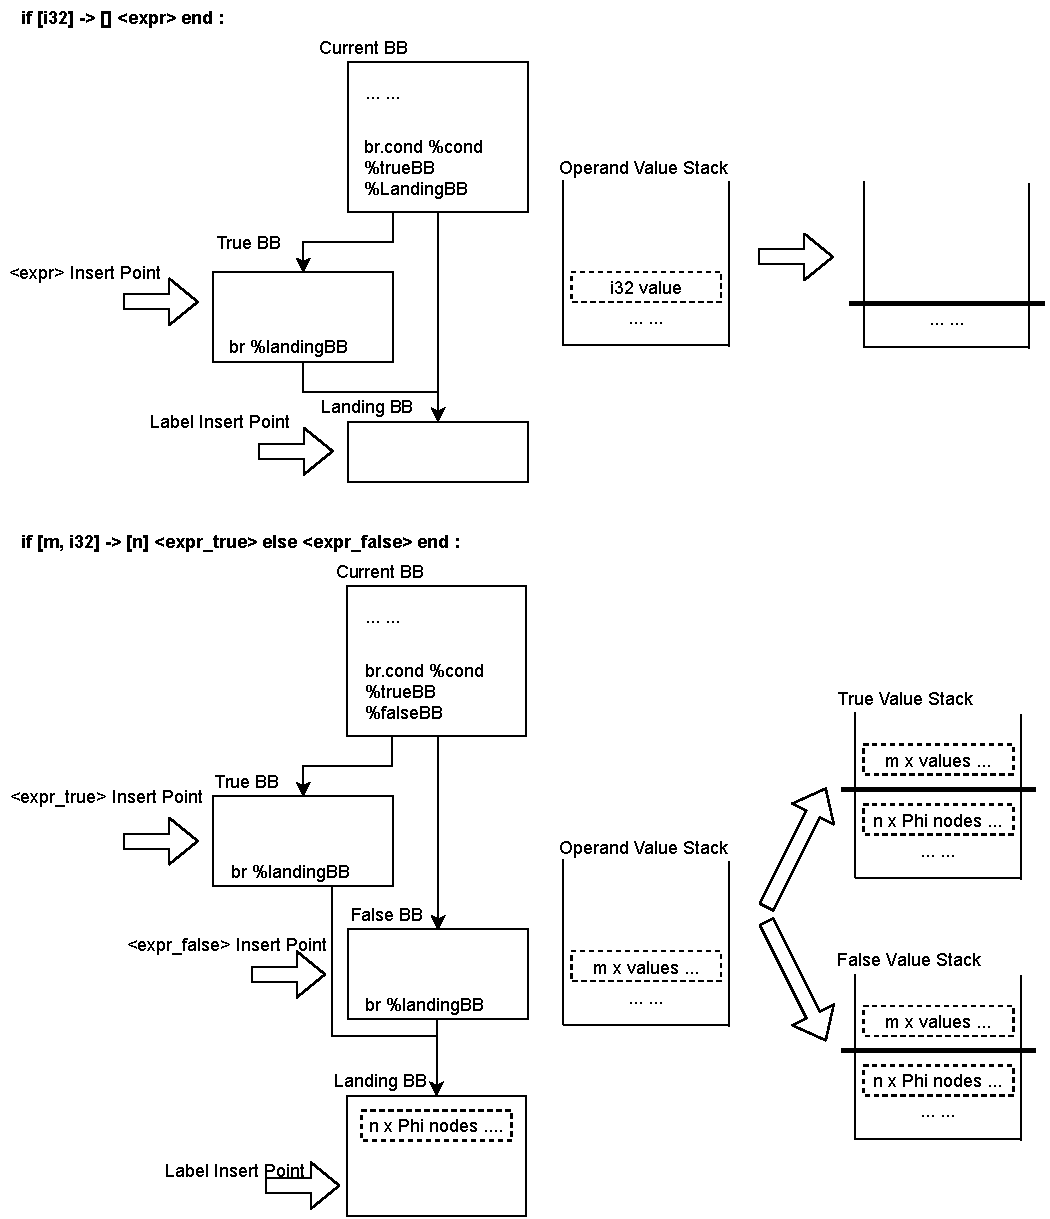
\includegraphics[width=\textwidth]{Images/4.MIR/translate-if.pdf}
  \caption{WebAssembly \texttt{if} translation pattern}
  \label{fig:translate-if}
\end{figure}

\paragraph{Block}
In the background chapter, we provide a general illustration of the three
structured control flow constructs. As a quick recap, \texttt{block} is the
simplest form of a structured control flow construct. It implicitly introduces
a label at the end of its enclosing instructions. A branch instruction
referring to this label will redirect the control flow to the end of the block.
Figure~\ref{fig:translate-block} illustrates the translation pattern for
WebAssembly \texttt{block} in SableWasm MIR. We will first clarify some of the
terminologies we used in the figure, and we will use the same terms later in
the \texttt{loop} and \texttt{if} pattern discussion for consistency.
\emph{Expr Insert Point} refer to the starting position for the generated
instructions when we recursively translate the instructions within the enclosing
expression of the \texttt{block} instruction. Furthermore,
\emph{Label Insert Point} refer to the position for generated instructions when
we finish the recursive translation and resume to the parent expression of the
\texttt{block} instruction. A \emph{label stack entry} is a tuple consisting of
a pointer to the landing basic block, a list of $\phi$ nodes expecting merge
values, and a pointer to the \emph{label insert point}. The translation pattern
for \texttt{block} is pretty simple; we continue on the current basic block and
prepare the landing basic block for the block instruction as a branch
instruction within the expression may refer to the label. Additionally, to fully
support multi-value extension in WebAssembly, we also need to prepare the $\phi$
nodes in the landing basic block. SableWasm generates the $\phi$ nodes based on
the type of the \texttt{block} instruction. WebAssembly validation rules ensure
that the expression within the \texttt{block} can access exactly $m$ values from
the stack and put $n$ values onto the stack. Finally, we will append an
unconditional branch to the landing basic block because in WebAssembly,
if the control flow reaches the bottom of the \texttt{block} expressions, it
will implicitly fall through. For the operand stack, we will first pop $m$
values from the stack as \texttt{block} instruction's type suggests and push the
$\phi$ nodes as the result values. Then, we need to set up the boundary between
the operand stack for the expression contained within the \texttt{block}.
Figure~\ref{fig:translate-block} represents this with the bold line in the
result operand value stack. The last step is to push the $m$ values back to the
stack, as they are passed to the expression within the \texttt{block}.


\paragraph{If}
The next control-flow structure defined WebAssembly is \texttt{if}.
WebAssembly's \texttt{if} is an expression instead of a statement that appears
in many other languages such as C. The \texttt{if} expression can yield some
values indicated by its type. Figure~\ref{fig:translate-if} illustrates the
translation patterns in SableWasm. There are two types of \texttt{if}
instruction defined in WebAssembly specification. The first case is a `partial'
\texttt{if} instruction, where it only contains the `true' branch. From
WebAssembly validation rules, it's easy to show that the only possible type is
\texttt{[i32]->[]}, even with the multi-value extension proposal. This implies
that the expression within the \texttt{if} instruction must start with an empty
operand stack. Hence, the translation pattern for the partial \texttt{if} is
quite straightforward: we only need to pop the condition value from the operand
stack and construct a conditional branch based on this value in the current
basic block. On the other hand, we also have `full' \texttt{if} instructions
with both `true' and `false' expressions. The validation rules ensure that both
expressions must have the same type. The translation pattern is more complex
compare to that of a `partial' \texttt{if}. In this case, we have to prepare the
landing basic block similar to what we did for the \texttt{block} construct.
We need to generate $n$ $\phi$ nodes for data-flow mergers from the `true'
branch, the `false' branch, and any possible branch instruction within both
nested expressions. Similarly, we need to pop $m$ values from the stack for
operand values stack and then push $n$ $\phi$ nodes. And, within both nested
expressions, push $m$ values back to the stack.

\begin{figure}
  \centering
  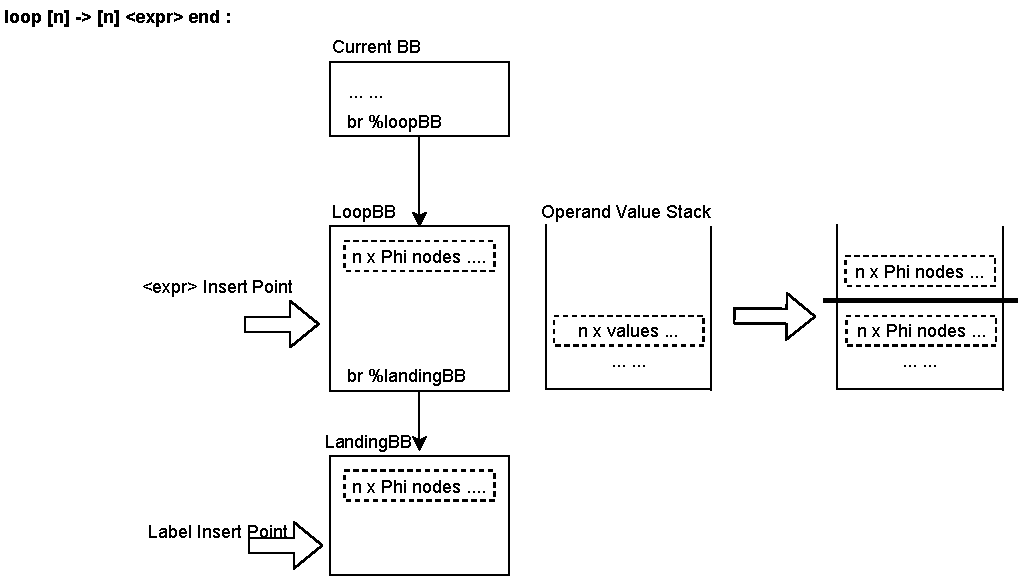
\includegraphics[width=\textwidth]{Images/4.MIR/translate-loop.pdf}
  \caption{WebAssembly \texttt{loop} translation pattern}
  \label{fig:translate-loop}
\end{figure}

\paragraph{Loop}
The last control-flow structure defined in WebAssembly is \texttt{loop}.
Figure~\ref{fig:translate-loop} gives a general illustration of SableWasm's
translation pattern for \texttt{loop} instructions. Similar to the `partial'
\texttt{if} we discussed in the previous paragraph, one can show that, under
WebAssembly's validation rules, the parameter types for the \texttt{loop}
instruction must equal to the result types. The \texttt{loop} instruction is
similar to the \texttt{block} instruction, except that if any branch
instruction refers to it, the branch instruction should transfer the control
flow to the start of the expression within the instruction instead of the end.
Thus, we need to prepare a standalone basic block for the nested expression in
\texttt{loop}, along with the $\phi$ nodes to merge value on each loop
iteration. Note that we also introduce $\phi$ nodes in the landing basic block.
One may argue that there is no need for these $\phi$ nodes, as only one block
can reach the loop exit, and no value merging will occur. Indeed, these
$\phi$ nodes will always be trivial $\phi$ nodes, which have only one
possible value inflow. However, this is due to the limitation of our translation
framework.

In this section, we discussed the translation patterns for WebAssembly
structured control flow constructs. Thanks to WebAssembly validation rules, the
types for these structured control flow instructions explicitly mark value
merging and imply possible $\phi$ nodes. Furthermore, one can show that the
control graph generated above is indeed in SSA form. However, the directly
generated control flow graph is not easily understandable by users. This mainly
comes from two facts. First, the WebAssembly-targeting compiler may generate
awkward patterns to fit in the structured control-flow constructs. Second,
SableWasm translation patterns for structured-control flow constructs are not
optimal.
\subsection{Instructions Reduction}

This section will cover the instructions reduction rules used when lowering WebAssembly bytecode to SableWasm MIR. In the background chapter, we mentioned that one of WebAssembly's design goals is to be as compact as possible. When the community design the WebAssembly instruction set, they fuse several typical instruction sequences into single instructions. For example, SIMD vector operation extension defines \texttt{v128.load8x8\_s} which first load 8 single-byte integers into a vector, and then sign-extended them into 16 bit integers. Another example will be \texttt{v128.load32\_lane} which loads a 32-bit value, either a 32-bit integer or a single-precision floating-point number into a given vector. Such design is understandable for WebAssembly as binary size do matter when shipping application over the internet. But, for SableWasm, a static compiler, we focus more on the size of the instruction set instead of the size of the intermediate representation. It is harder to write analysis for a bloated instruction set, as one needs to consider more instruction cases. Hence, when lowering WebAssembly bytecode to SableWasm MIR, we replace some WebAssembly instructions with a sequence of SableWasm MIR instructions.


\paragraph{Eqz} \quad
\begin{lstlisting}[basicstyle=\linespread{1}\small, language=LLVM]
[..., %n i32] i32.eqz => %t0 = i32.const 0; %t1 = int.eq %n %t0
[..., %n i64] i64.eqz => %t0 = i64.const 0; %t1 = int.eq %n %t0
\end{lstlisting}
WebAssembly defines unary \texttt{eqz} operations for all integer values. As the name suggests, \texttt{eqz} compares the operand value against zero and yields to one if true, zero otherwise. In SableWasm MIR, we group all comparison instructions into \texttt{Compare} class, and \texttt{eqz} does not fit into the class as it is not a binary operation. Hence we rewrite the \texttt{eqz} as \texttt{Compare} instruction with opcode as \texttt{Eq}.

\paragraph{Load} \quad
\begin{lstlisting}[basicstyle=\linespread{1}\small, language=LLVM]
[..., %base i32] i32.load offset=%offset align=%align =>
    %addr = int.add %base %offset;
    memory.guard %mem %addr 4;
    %t0 = load.32 i32 %mem %addr
[..., %base i32] i32.load16_u offset=%offset align=%align =>
    %addr = int.add %base %offset;
    memory.guard %mem %addr 2;
    %t0 = load.16 i32 %mem %addr
[..., %base i32] i32.load16_s offset=%offset align=%align =>
    %addr = int.add %base %offset;
    memory.guard %mem %addr 2;
    %t0 = load.16 i32 %mem %addr;
    %t1 = cast i32.extend.16.s %t0
\end{lstlisting}



\section{Analysis Framework}
\begin{figure}
  \centering
  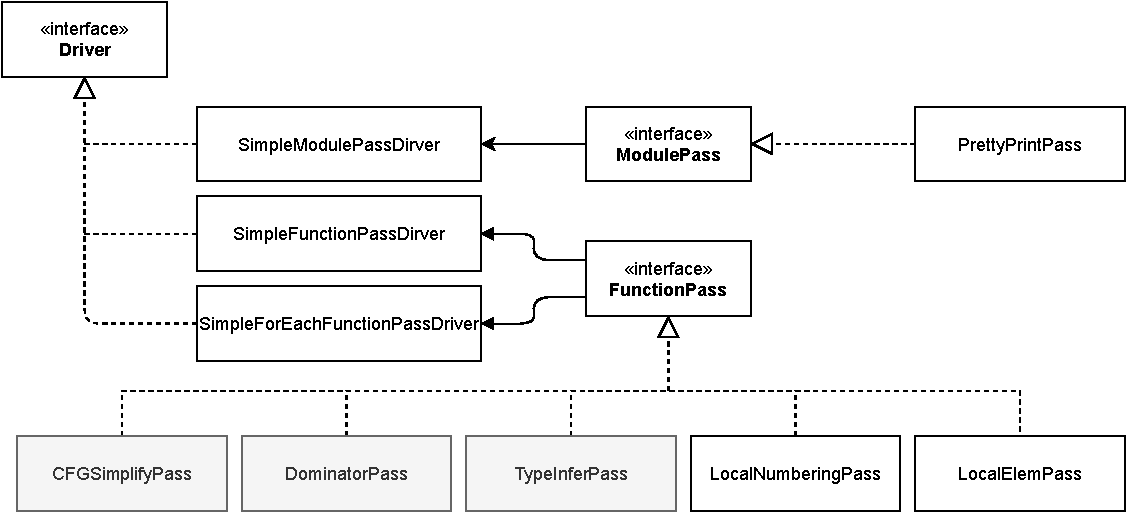
\includegraphics[width=\textwidth]{Images/4.MIR/analysis-framework.pdf}
  \caption{SableWasm MIR Analysis and Optimization Framework}
  \label{fig:sablewasm-mir-analysis-framework}
\end{figure}
SableWasm also implements an analysis and optimization framework over middle-level intermediate representation (MIR). The framework consists of two parts, passes and drivers. SableWasm analysis and transformation framework only provides essential support for managing passes, compared to other more advanced frameworks, such as McSAF\cite{mcsaf}, an optimization framework for MATLAB language. Figure~\ref{fig:sablewasm-mir-analysis-framework} illustrates the current state of the framework in SableWasm. Currently, we implement three different drivers. \texttt{SimpleModulePassDirver} accepts module passes and operates on the module level. At the time of thesis writing, we haven't explored the inter-procedure analysis for SableWasm MIR in detail, and the only module pass implemented is the pretty print pass.

\subsection{Control-Flow Graph Simplification}

\subsection{Dominators and Dependence}

\subsection{Type Infer}

\subsection{Local Value Numbering}

\subsection{Redundant Local Variable Elimination}
\chapter{Backend and Runtime}

This chapter discusses the last component of the SableWasm compilation pipeline, the code generation backend and runtime support for generated shared libraries. Currently, SableWasm has only one backend based on the LLVM compiler infrastructure. However, in the future, one can easily extend the system by adding more backends that lowering SableWasm MIR into other intermediate representations. Another problem that appears when designing a backend is how SableWasm MIR entities map to native constructs. In SableWasm, we take an instance-based approach. The SableWasm runtime library will manage all entities in an instance object. The system will pass it to the generated native functions as the first argument, similar to `this' pointer in many C++ implementations. In the rest of the chapter, we will first go through the design of the instance object, followed by implementation of WebAssembly entities. Finally, we will discuss the code generation strategies used when lowering SableWasm MIR to LLVM intermediate representation and the interaction between generated shared libraries and the hosting language.

\section{Instance Layout}

\begin{figure}
    \begin{minipage}{.35\textwidth}
        \centering
        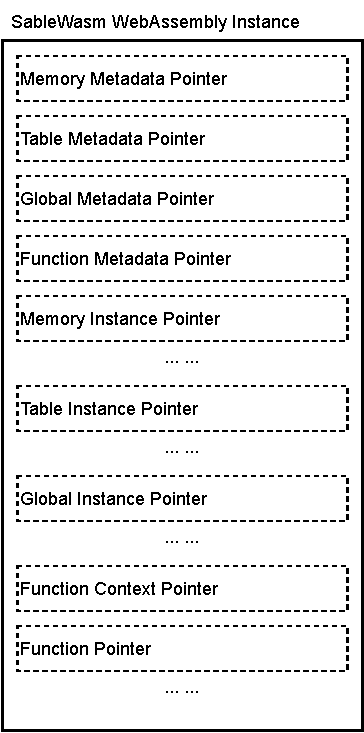
\includegraphics[width=\textwidth]{Images/5.Backend_and_Runtime/instance}
    \end{minipage}\hfill
    \begin{minipage}{.6\textwidth}
        \begin{lstlisting}[language=C, basicstyle=\ttfamily\footnotesize]
struct instance {
    memory_metadata_t   *memory_metadata;
    table_metadata_t    *table_metadata;
    global_metadata_t   *global_metadata;
    function_metadata_t *function_metadata;
    memory_t            *memories[NUM_MEMORY];
    table_t             *tables[NUM_TABLE];
    global_t            *globals[NUM_GLOBAL];
    struct {
        struct instance *context;
        function_t      *function_ptr;
    } * functions[NUM_FUNCTIONS];
};        
    \end{lstlisting}
    \end{minipage}
    \caption{SableWasm WebAssembly Instance}
    \label{fig:backend-instance}
\end{figure}

This section discusses the WebAssembly instance implementation in SableWasm. A WebAssembly instance hosts all the runtime structures that the generated shared libraries require, such as linear memory and indirect table. Figure~\ref{fig:backend-instance} illustrates the design of the WebAssembly instance. SableWasm's WebAssembly instance consists of two parts, metadata entries and entity pointers. One may also notice that the instance object's size may vary from modules to modules depending on how many entities are declared. This behaviour is intensional by design. SableWasm runtime system needs to compute the address of the pointers based on the metadata information on the fly. By packing all pointers in a consecutive memory region, we reduce one layer of indirection for the runtime system, and in theory, may improve runtime performance. On the other hand, the generated shared library has all the entities address inlined as the backend can infer them during code generation, which does not incur any performance loss. For most of the entities, they are pretty straightforward, and we will skip the discussion here. In the rest of the section, we focus on three aspects: the metadata entries, the function entity representations, and the instance initialization protocol in SableWasm.

\paragraph{Metadata}
One could think of the metadata as the signatures for entities, and indeed, the SableWasm runtime system prepares the instance object based on the metadata. Further, shared libraries generated by SableWasm only publicly expose the metadata and initialization function to conceal module details. Metadata encodes the type for the entity. For linear memories and indirect tables, this is relatively trivial as their types only consist of an integer pair. In the case of global values, things are a little bit complicated. A quick reminder, WebAssembly global types keep track of their value type and mutability. The first problem here is how to encode WebAssembly value types. One solution is to use WebAssembly value type binary format. However, this encoding strategy emits hard to maintain results as a human can not directly read them. Here we use the JVM approach for value type encoding \footnote{\url{https://docs.oracle.com/javase/7/docs/technotes/guides/jni/spec/types.html}}. A quick summary, in SableWasm, we encode 32-bit integers as `I', 64-bit integers as 'J', single-precision floating-point number as 'F', double-precision floating-point number as 'D' and finally, 128-bit vector type as 'V'. The second problem is how to encode global's mutability. In SableWasm, we use capital letters for constant global value types and lower letters for mutable ones. Finally, for function types, we follow a similar design as we used for global values. SableWasm encodes function type into a null-terminated string. Let's take \texttt{[i32, f32] -> [v128]} as an example. SableWasm encodes the type into `\texttt{IF:V}'. The colon acts as a separator between parameter types and result types. Note that `\texttt{:}' itself is also a valid SableWasm function type string, and represents \texttt{[] -> []}, a void function with no arguments. Finally, metadata also encode module names and entity names for import entities and names for export names, which play a critical role later in the module initialization phase.

\paragraph{Function entity representation}
WebAssembly specifications classify the functions into two groups, WebAssembly functions and host functions. WebAssembly functions are any functions defined within the module. On the other hand, the runtime system provides host functions to the module, and from the WebAssembly module point of view, the functions are black boxes without any knowledge of their internals. To make things more complex, although, in MVP WebAssembly, there are no explicit requirements on how the WebAssembly functions should behave if they are invoked from other modules. Here we use a similar generalization in Javascript \footnote{WebAssembly Javascript Interface: \url{https://www.w3.org/TR/wasm-js-api-1/}}. In summary, in SableWasm, if a module exports a function, it exports the function in a closure that captures its enclosing instance. Suppose a second module invokes the exported closure via import functions. In that case, the function still only has access to its original module's entities and only communicates with the second module via return values. Hence, in SableWasm, we implement our function as a pair of pointers. The first one refers to its enclosing instance, and the second one refers to pointers to the generated code. For host functions, we set the enclosing instance as a null pointer. In the chapter's introduction, we mentioned that we pass the instance object as the first argument to the generated functions. But, what should we pass to the host functions? SableWasm defines that for all the host functions, the instance object will always point to the caller's enclosing instance instead of null so that the host functions can access the internals of the caller's module.

\paragraph{Initialization protocol}
In the last part of the section, we will cover the initialization protocol we used in SableWasm. The initialization protocol consists of three basic steps, validation, instance preparation and initialization. In the validation phase, we load the shared library with the operating system's help, such as \texttt{dlopen} in Linux, and check if it contains all the required symbols. Currently, a SableWasm shared library needs to export five symbols in total. Table~\ref{table:sablewasm-runtime-export-syms} illustrates the symbols expected from the generated shared libraries. The instance initializer function takes a prepared instance object as the argument. The next step in SableWasm is to construct this prepared instance object. The idea of a prepared instance object is that we want to separate the memory allocation from the value initialization. In SableWasm, the runtime system handles the memory allocation, while on the other hand, the initializer function takes care of the value initialization. In the second phase, the SableWasm runtime allocates all the entities and attaches them to the module instance. Note that SableWasm also resolves all the import names at this stage, and it will only proceed to the next step if all the expecting import entities are set. Finally, the last step is the initialization. SableWasm will invoke the initializer function provided by the shared library. The initializer function takes care of all kinds of value initialization, such as setting values for global variables and copy data segments into linear memory.

\begin{table}[h]
    \centering
    \begin{tabular}{|l|l|}
        \hline
        \textbf{Symbol Name}          & \textbf{Description}         \\ \hline
        \_\_sable\_global\_metadata   & Metadata for global values   \\ \hline
        \_\_sable\_memory\_metadata   & Metadata for linear memories \\ \hline
        \_\_sable\_table\_metadata    & Metadata for indirect tables \\ \hline
        \_\_sable\_function\_metadata & Metadata for functions       \\ \hline
        \_\_sable\_initialize         & Instance initializer         \\ \hline
    \end{tabular}
    \caption{SableWasm shared libraries exported symbols}
    \label{table:sablewasm-runtime-export-syms}
\end{table}
\section{WebAssembly Entities}

In the previous section, we discuss the design of the SableWasm WebAssembly instance object. However, we treat all WebAssembly entities' implementation as an opaque pointer without diving into the details during the last section. This section will cover the implementation of the WebAssembly entities along with the runtime library support functions exposed to the generated code in SableWasm. Before we start this section, we will first present the terms used throughout the later part of the thesis. In the rest of the chapter, we use \texttt{\_\_sable\_instance\_t} to denote the type of the instance object. Similarly, we use a similar format when talking about WebAssembly linear memory, indirect table and global variables. For example, \texttt{\_\_sable\_instance\_t} is the type of SableWasm's WebAssembly linear memory implementation. Finally, we use \texttt{\_\_sable\_function\_t} refer to the function pointers that point to generated native functions.

\paragraph{Linear Memory}

\begin{figure}
    \centering
    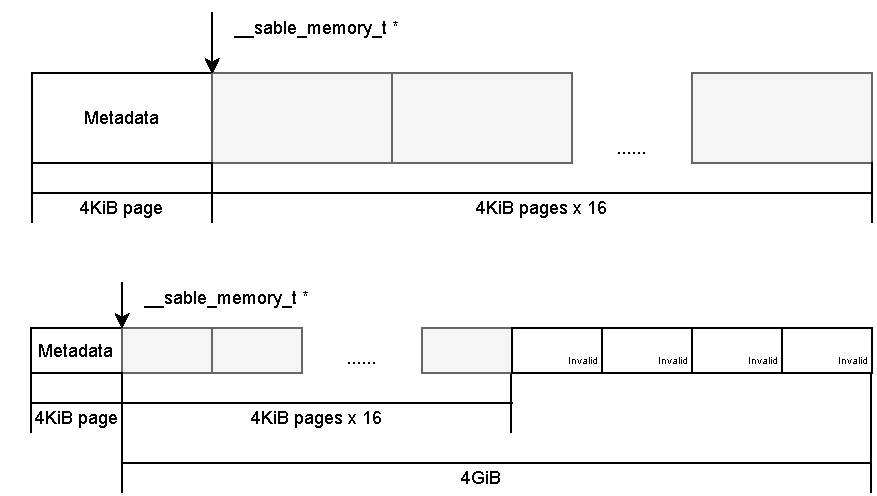
\includegraphics[width=0.85\textwidth]{Images/5.Backend_and_Runtime/memory}
    \caption{SableWasm WebAssembly linear memory}
    \label{fig:backend-memory}
\end{figure}

SableWasm implements WebAssembly linear memory with mapped memory provided by the operating system. It also has a fallback implementation that uses standard \texttt{malloc} and \texttt{free} procedure from the C library for an operating system that does not support mapped memory. The fallback implementation is relatively trivial, and we will not discuss it in the thesis. Here, we will focus on the one that uses mapped memory. Figure~\ref{fig:backend-memory} illustrates the strategies when mapping WebAssembly linear memory into native memory. On the top, we have a linear memory with a size of 1 in WebAssembly page size. In the figure, we assume the native machine has a page size of 4KiB, which is typical for most hardware architectures. A quick recap on the requirements of WebAssembly linear memory. First, the program can efficiently random access any location within the linear memory. Second, at runtime, the module function can query the size of the linear memory. Finally, the program can grow the linear memory if the runtime system allows it. SableWasm implements the linear memory using a similar trick as the one used for `\texttt{malloc}' functions in many C standard library implementations. From the generated shared libraries' point of view, the linear memory object points to the start of a continuous memory chunk. Hence, memory accesses are efficient and require only one layer of indirection. First, the generated function will fetch the linear memory base pointer from the instance object and perform offset calculation accordingly. An extra page manages the metadata of the linear memory at the beginning. It contains all the records that the runtime system needs to work with the linear memory, such as the current size and the upper bound. Note that the size of the metadata is usually way smaller than the page size defined by the native machine. Still, SableWasm reserves a whole page for it, as we want our linear memory start address to be always page-aligned in the hope of better performance.

\begin{table}[h]
    \centering
    \begin{tabular}{|l|l|l|}
        \hline
        \textbf{Runtime support functions} & \textbf{Return Value} & \textbf{Arguments}                \\ \hline
        \_\_sable\_memory\_size            & uint32\_t             & \_\_sable\_memory\_t *            \\ \hline
        \_\_sable\_memory\_guard           & void                  & \_\_sable\_memory\_t *, uint32\_t \\ \hline
        \_\_sable\_memory\_grow            & uint32\_t             & \_\_sable\_memory\_t *, uint32\_t \\ \hline
    \end{tabular}
    \caption{SableWasm runtime support functions for linear memory}
    \label{tbl:sablewasm-runtime-memory-api}
\end{table}

SableWasm implements additional functionality through library functions. Table~\ref{tbl:sablewasm-runtime-memory-api} illustrates all the runtime library support functions provided by SableWasm. \texttt{\_\_sable\_memory\_size} implements SableWasm's \texttt{MemorySize} instruction. It takes an argument of linear memory instance and returns the size of it in WebAssembly page size. The second runtime support function, \texttt{\_\_sable\_memory\_guard} corresponds to the \texttt{MemoryGuard} instructions in SableWasm. It takes the arguments of a linear memory instance and the expected number of bytes ahead. Note that the function does not return any values, and this is intentional by design. SableWasm runtime library utilizes the C++ exception mechanism to report and handle errors. If the memory access is out-of-bound, the runtime system will throw an exception. We will come back to this later in the chapter when discussing the interaction between the generated shared libraries and the host language. Finally, the last runtime support function, \texttt{\_\_sable\_memory\_grow} implements the SableWasm's \texttt{MemoryGrow} instruction. The instruction follows its counterpart that appeared in WebAssembly specification. It takes a linear memory instance and the number of pages to increase as arguments. If the operation is successful, the function will yield to the new size of the linear memory; otherwise, it returns -1 instead. SableWasm grows the memory by remmaping the memory with the help of the oeprating system. On Linux, this usually corresponds to a \texttt{mremap} operation.

In the above implementation, all linear memory-bound checks are program-directed, and they are relatively quite expensive. To further improve the performance, we use a similar technique used by many virtual machine implementations, which utilizes mapped memory access flags. Figure~\ref{fig:backend-memory} illustrates this approach at the bottom. One may notice that MVP WebAssembly works with 32-bit addressing \footnote{This is subject to change in the future. WebAssembly 64-bit memory addressing:\\\url{https://github.com/WebAssembly/memory64}}. Hence, the maximum size of the linear memory is 4GiB. Thus, SableWasm reserves 4GiB of address when allocating the linear memory and marks all the pages beyond the current range as invalid pages.  This operation is quite efficient as we only work with the memory address instead of allocating the memory. In this implementation, any out-of-bound will result in a memory segmentation fault. Note that this strategy does yield better performance but results in a nonrecoverable error. SableWasm provides both implementations, and one can select based on their needs. In the next chapter, when we compare SableWasm's performance against several other implementations. We always use the second strategy, as the recoverable code is not a requirement.

\paragraph{Global}

\paragraph{Indirect Table}

\section{Code Generation}

\section{Interface with C/C++}

\chapter{Evaluation}

In the previous chapters, we present the design of the SableWasm compiler and runtime. This chapter will focus on the performance evaluation in terms of the execution speed of the generated shared libraries. Here, we focus on three research problems. First, how does SableWasm performs compares to other WebAssembly runtime environment implementations? Second, does the optimization over the input WebAssembly module affect the overall performance? Finally, how much does the WebAssembly SIMD extension improve comparing to optimized scalar counterparts? We will first present the setup for experiments used when investigating three questions, and later, the experiment results for each one of them.

\section{Experiment Setup}

This section presents the setup for the experiments in the remaining part of the chapter. We conduct the benchmarks on the same server for all experiments. The server has a The experiments were performed on a six-core Intel Core processor at a 3.7 GHz standard clock frequency and an L3 cache of 12 MiB. Additionally, The server runs Ubuntu 18.04 with Linux kernel version 4.15.0 and 32GiB of memory. When measuring the performance, we execute each benchmark ten times in succession to minimize the measurement error as some of the benchmarks take less than a second to complete. Finally, the final benchmark result is the average among ten runs except the highest and the lowest. For the benchmark subject, we choose three different benchmark suits, the Polyhedral benchmark suite (Polybench), the Ostrich benchmark suite (Ostrich) and the NAS parallel benchmarks (NPB).

\begin{table}
    \centering
    \begin{tabular}{|l|l|}
    \hline
    \textbf{Benchmark Name} & \textbf{Description}                                \\ \hline
    2mm                     & 2 matrix multiplication (D = A.B; E = C.D)          \\ \hline
    3mm                     & 3 matrix multiplication (E = A.B; F = C.D; G = E.F) \\ \hline
    adi                     & alternating direction implicit solver               \\ \hline
    atax                    & matrix transpose followed by vector multiplication  \\ \hline
    bicg                    & BiCG sub kernel of BiCGStab linear solver           \\ \hline
    cholesky                & Cholesky decomposition                              \\ \hline
    correlation             & correlation computation                             \\ \hline
    covariance              & covariance computation                              \\ \hline
    doitgen                 & multiresolution analysis kernel (MADNESS)           \\ \hline
    durbin                  & Toeplitz system solver                              \\ \hline
    dynprog                 & dynamic programming (2D)                            \\ \hline
    fdtd-2d                 & 2D finite different time domain kernel              \\ \hline
    fdtd-apml               & FDTD using anisotropic perfectly matched layer      \\ \hline
    gauss-filter            & gaussian filter                                     \\ \hline
    gemm                    & matrix-multiply (C = alpha.A.B + beta.C)            \\ \hline
    gemver                  & vector multiplication and matrix addition           \\ \hline
    gesummv                 & scalar, vector and matrix multiplication            \\ \hline
    gramschmidt             & Gram-Schmidt decomposition                          \\ \hline
    jacobi-1D               & 1D Jacobi stencil computation                       \\ \hline
    jacobi-2D               & 2D Jacobi stencil computation                       \\ \hline
    lu                      & LU decomposition                                    \\ \hline
    ludcmp                  & LU decomposition (different implementation)         \\ \hline
    mvt                     & matrix vector product and transpose                 \\ \hline
    reg-detect              & 2D image processing                                 \\ \hline
    seidel                  & 2D Seidel stencil computation                       \\ \hline
    symm                    & symmetric matrix multiplication                     \\ \hline
    syr2k                   & symmetric rank-2k operations                        \\ \hline
    syrk                    & symmetric rank-k operations                         \\ \hline
    trisolv                 & triangular solver                                   \\ \hline
    trmm                    & triangular matrix multiplication                    \\ \hline
\end{tabular}
    \caption{the Polyhedral benchmark suite (Polybench)}
    \label{tbl:polybench}
\end{table}

\paragraph{Polybench}
The Polyhedral benchmark suite (Polybench) \cite{polybench} contains a group of small math kernel functions as shown in table~\ref{tbl:polybench}. The description table is adjusted from official Polybench documentation\footnote{Polybench: \url{http://web.cse.ohio-state.edu/~pouchet.2/software/polybench/}}. In the WebAssembly announcement paper \cite{10.1145/3062341.3062363}, the community also chooses Polybench as the evaluation subject. However, one problem is that the Polybench is in C. Therefore, the researchers cross-compile the benchmark using a modified Clang compiler with LLVM WebAssembly backend. However, there is no standardized system interface, such as WASI, proposed by the community when publishing the paper. Hence, the experiment is measured with an external clock, and all features that require system interaction are disabled. On the other hand, when evaluating SableWasm, we use a WASI-enabled Clang compiler \footnote{WASI SDK: \url{https://github.com/WebAssembly/wasi-sdk}} to cross-compile the WebAssembly modules into WebAssembly modules. Each benchmark reports its execution time by issuing syscalls to the runtime environment, which in theory, should yield more accurate results, especially for a just-in-time (JIT) runtime environment.

\begin{table}
    \centering
    \begin{tabular}{|l|l|}
    \hline
    \textbf{Benchmark Name} & \textbf{Description}                                        \\ \hline
    back-prop               & backward propagation in a layered neural network            \\ \hline
    bfs                     & breadth-first search in a randomly generated graph          \\ \hline
    crc                     & CRC error-detecting algorithm                               \\ \hline
    fft                     & fast Fourier transform                                      \\ \hline
    hmm                     & forward-backward algorithm over a hidden Markov model       \\ \hline
    lavamd                  & 3D space particle simulation                                \\ \hline
    lud                     & LU decomposition                                            \\ \hline
    nqueens                 & N-queen problem solver                                      \\ \hline
    nw (needle)             & find optimal alignment of two protein sequences             \\ \hline
    page-rank               & page-rank algorithm to measure the importance of a web site \\ \hline
    spmv                    & sparse matrix multiplication with a vector                  \\ \hline
    srad                    & diffusion method for ultrasonic and radar imaging           \\ \hline
\end{tabular}
    \caption{the Ostrich benchmark suite (Ostrich)}
    \label{tbl:ostrich}
\end{table}

\paragraph{Ostrich}
The second benchmark suite we used in the Ostrich benchmark suite\cite{ostrich}, illustrated in table~\ref{tbl:ostrich}. Comparing to the Polybench, Ostrich focuses on larger scientific problems instead of computation kernels. Ostrich benchmark suite supports multiple programming languages, such as Javascript and C. Here, we prepare the WebAssembly module similar to the Polybench benchmark suite with a WASI-enable Clang compiler. However, unlike the Polybench benchmark suite, which does not require any modification on the source code, we need to tweak the Ostrich benchmark code due to the limitation of WebAssembly specification. This includes hard-coding the command-line arguments and replacing throwing an exception with calling \texttt{exit} function.

\begin{table}
    \centering
    \begin{tabular}{|l|l|}
    \hline
    \textbf{Benchmark Name} & \textbf{Description}                                 \\ \hline
    IS                      & integer sort (bucket sort)                           \\ \hline
    EP                      & Marsaglia polar method for generating random numbers \\ \hline
    CG                      & estimate the smallest eigenvalue of a SPD matrix     \\ \hline
    MG                      & multi-grid on a sequence of meshes                   \\ \hline
    FT                      & fast Fourier transform                               \\ \hline
    BT                      & block tri-diagonal solver                            \\ \hline
    SP                      & scalar penta-diagonal solver                         \\ \hline
    LU                      & lower-upper solver                                   \\ \hline
\end{tabular}
    \caption{the NAS parallel benchmark suite (NPB)}
    \label{tbl:npb}
\end{table}

\paragraph{NPB}
The last benchmark suite we selected for evaluating SableWasm is the NAS parallel benchmark suite \cite{npb}, shown in the table~\ref{tbl:npb}. We choose this benchmark because of its parallel nature, as the third research question focuses on the SIMD instruction operations. However, the original NPB benchmark suite is in Fortran, and, at the time of thesis writing, there is no cross-compiler from Fortran to WebAssembly. Hence, we choose an OpenMP variant instead \footnote{NPB OpenMP C: \url{https://github.com/benchmark-subsetting/NPB3.0-omp-C}}. Although the currently WASI-enable Clang does not support OpenMP, we can still cross-compile into WebAssembly, as OpenMP code trivially reduces to C.

This section presents the benchmark environment and test cases for the experiment later in the chapter. One may notice some duplication among three benchmark suites, such as the upper-lower matrix decomposition (LU, ludcmp) and fast Fourier transform (FT, fft). However, we will still treat them as different individual test cases for all of them, as they come with various implementations and may lead to performance differences. Another problem that arises when preparing WebAssembly modules for benchmark suits is that some of the generated modules from the WASI-enabled Clang compiler have unexpected behaviour. In NPB, although the WASI-enabled Clang compile can successfully translate all test cases for all eight benchmark cases, there are two among eight test cases that have different behaviour compare to their native counterparts. For example, the WebAssembly module for the IS benchmark case has memory access out-of-bound for native and optimized translation. Also, the module for EP failed when compiled with the optimization flag enabled in the WASI-enabled Clang compiler. We suspect that some unknown bug in the toolchain may exist as it is still under active development. Another possible cause for the problem is that the OpenMP implementation may contain non-standard operations that result in undefined behaviour. We also test the generated modules against several other WebAssembly runtime environments, and the result is consistent. The last problem we encounter during benchmark is around WebAssembly SIMD operation extensions. As the extension is still under standardization, most runtime environments only support a subset of all instructions. Hence, when comparing SIMD operations, some of the benchmark results are infeasible. However, we still manage to collect SIMD operation performance data for most of the benchmark cases.

\section[RQ1: How does SableWasm perform compare to others?]{{\large RQ1: How does SableWasm perform compare to others?}}

\begin{figure}
    \centering
    \begin{subfigure}[t]{\textwidth}
        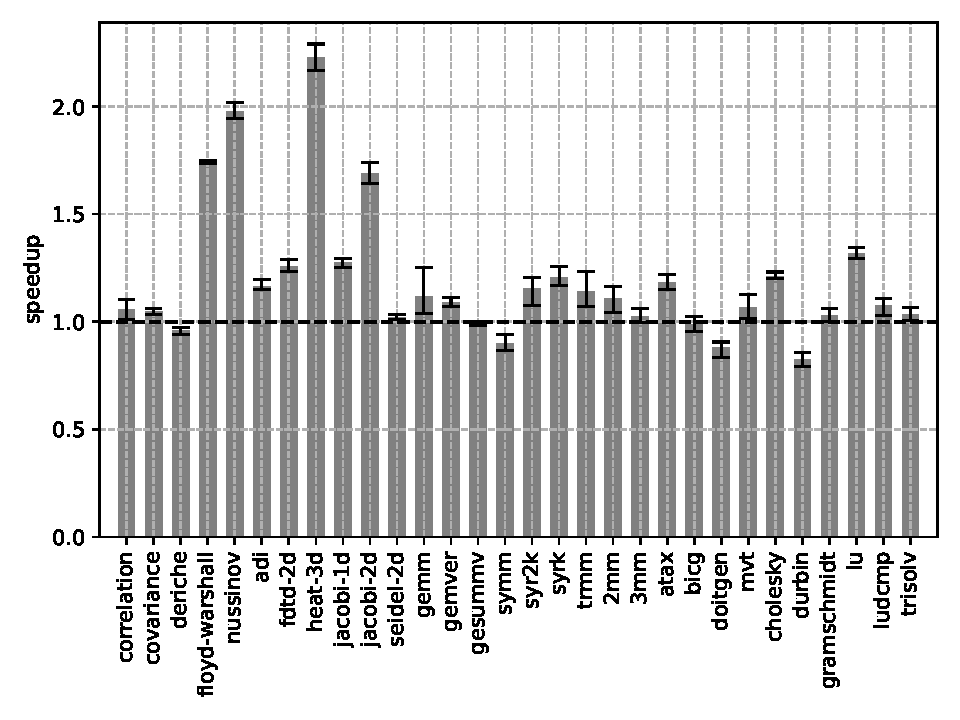
\includegraphics[width=\textwidth]
        {Images/6.1.RQ1/polybench-wasmtime-naive.pdf}
        \caption{Polybench}
    \end{subfigure}
    \begin{subfigure}[t]{.45\textwidth}
        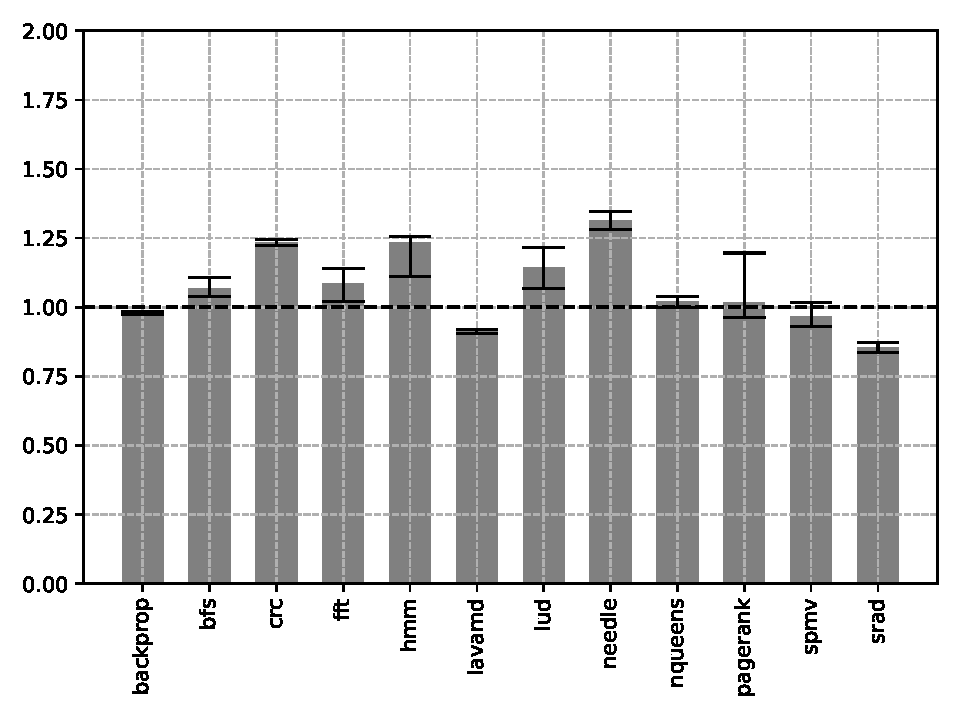
\includegraphics[width=\textwidth]
        {Images/6.1.RQ1/ostrich-wasmtime-naive.pdf}
        \caption{Ostrich}
    \end{subfigure}
    \begin{subfigure}[t]{.45\textwidth}
        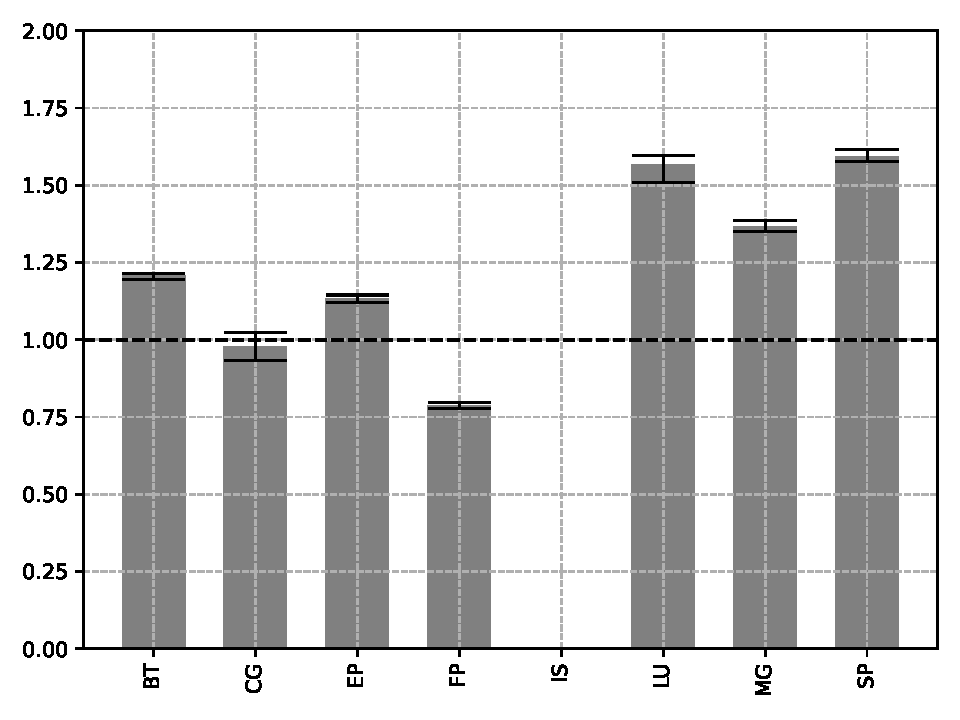
\includegraphics[width=\textwidth]
        {Images/6.1.RQ1/npb-wasmtime-naive.pdf}
        \caption{NPB}
    \end{subfigure}
    \caption{Benchmarks with naive (\texttt{-O0}) on Wasmtime}
    \label{fig:rq1-wasmtime-naive}
\end{figure}

\begin{figure}
    \centering
    \begin{subfigure}[t]{\textwidth}
        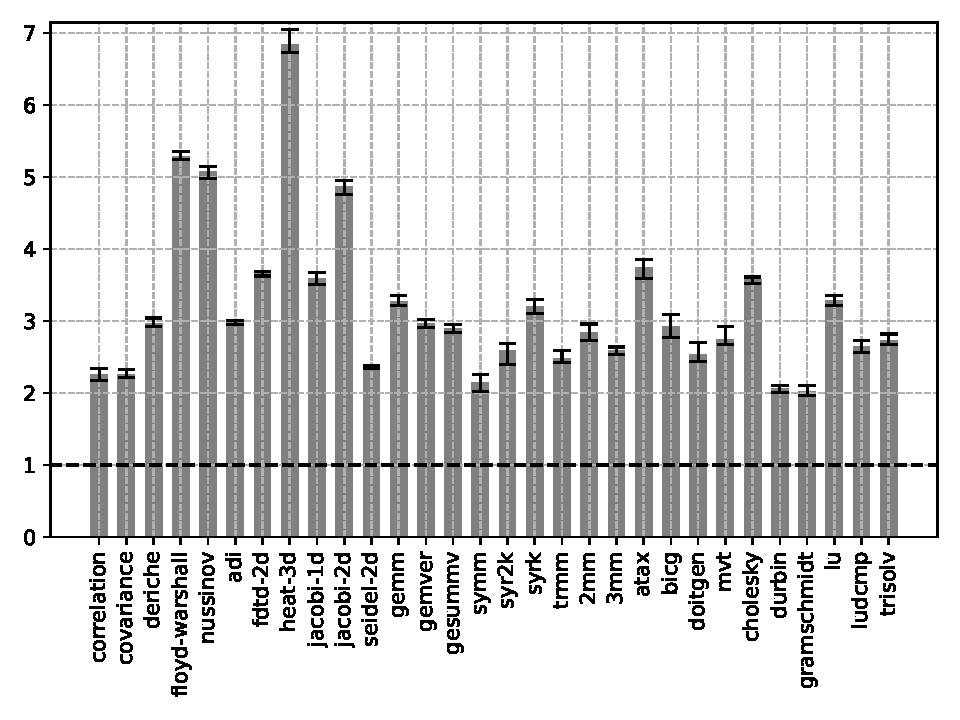
\includegraphics[width=\textwidth]
        {Images/6.1.RQ1/polybench-wasmer-cranelift-naive.pdf}
        \caption{Polybench}
    \end{subfigure}
    \begin{subfigure}[t]{.45\textwidth}
        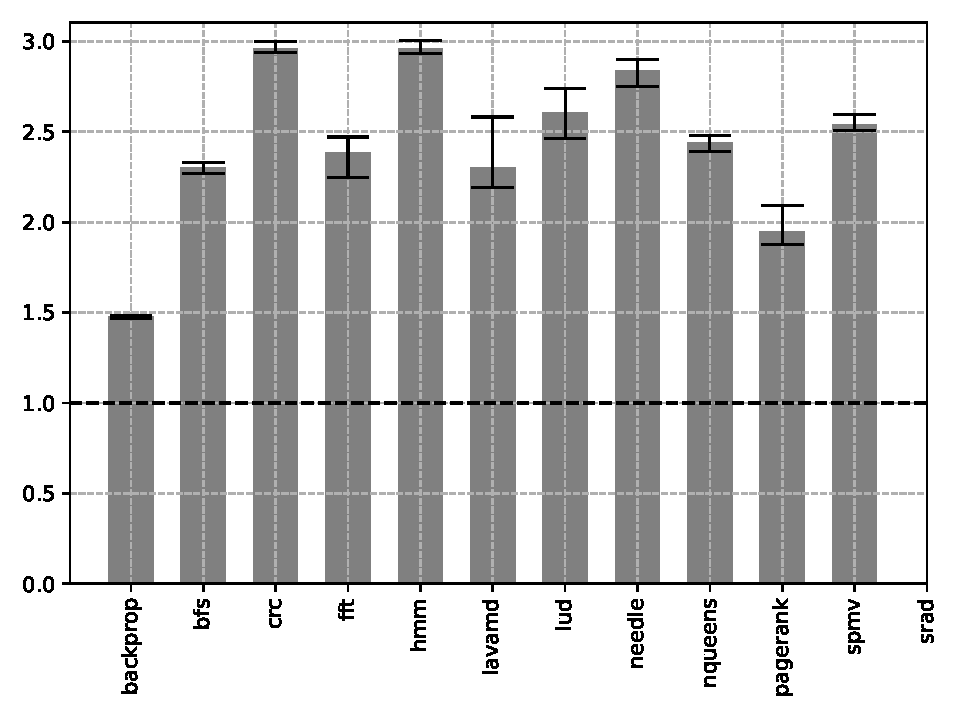
\includegraphics[width=\textwidth]
        {Images/6.1.RQ1/ostrich-wasmer-cranelift-naive.pdf}
        \caption{Ostrich}
    \end{subfigure}
    \begin{subfigure}[t]{.45\textwidth}
        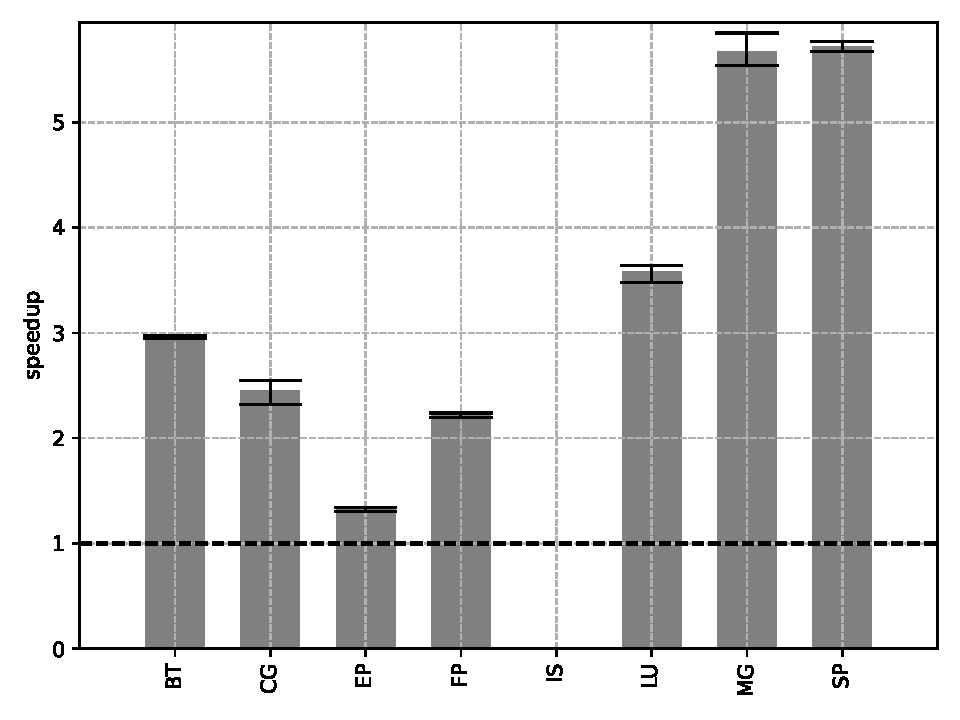
\includegraphics[width=\textwidth]
        {Images/6.1.RQ1/npb-wasmer-cranelift-naive.pdf}
        \caption{NPB}
    \end{subfigure}
    \caption{Benchmarks with naive (\texttt{-O0}) on Wasmer(Cranelift)}
    \label{fig:rq1-wasmer-cranelift-naive}
\end{figure}

\begin{figure}
    \centering
    \begin{subfigure}[t]{\textwidth}
        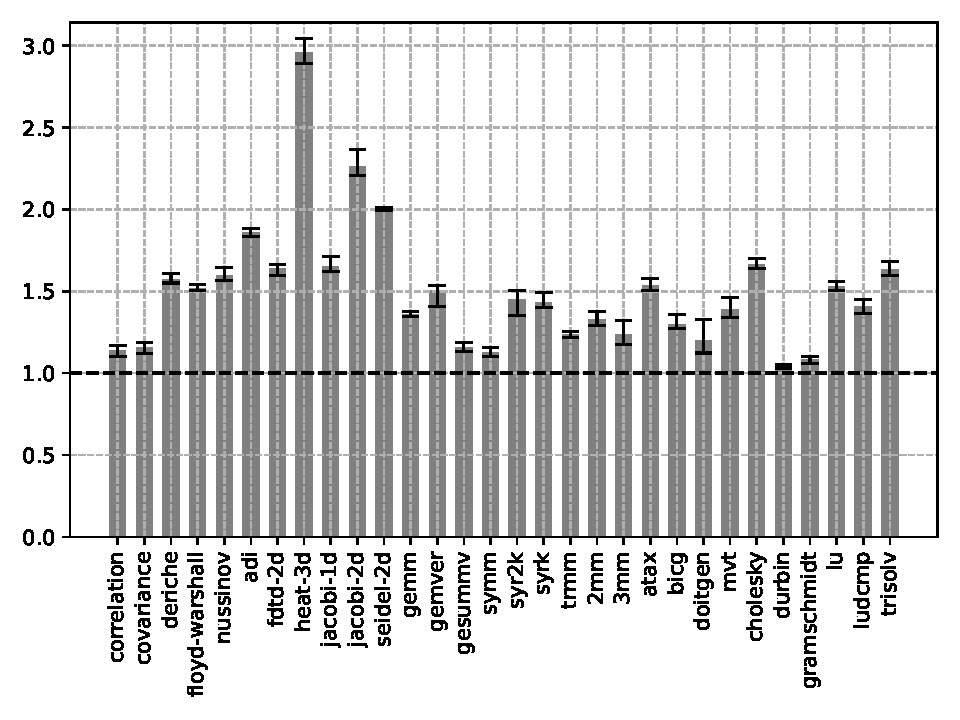
\includegraphics[width=\textwidth]
        {Images/6.1.RQ1/polybench-wasmer-llvm-naive.pdf}
        \caption{Polybench}
    \end{subfigure}
    \begin{subfigure}[t]{.45\textwidth}
        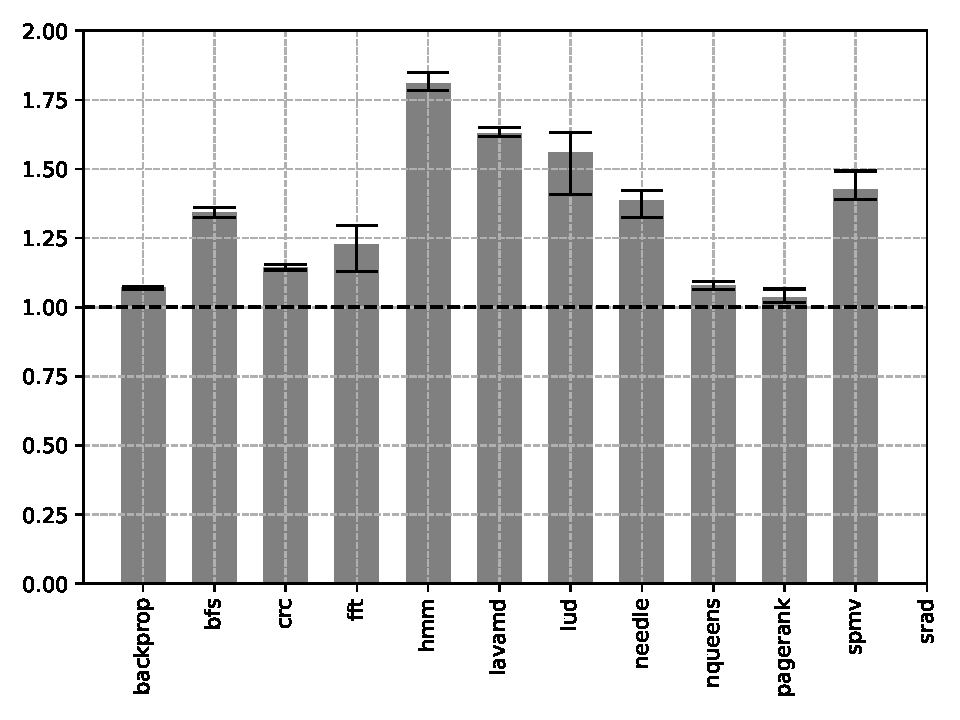
\includegraphics[width=\textwidth]
        {Images/6.1.RQ1/ostrich-wasmer-llvm-naive.pdf}
        \caption{Ostrich}
    \end{subfigure}
    \begin{subfigure}[t]{.45\textwidth}
        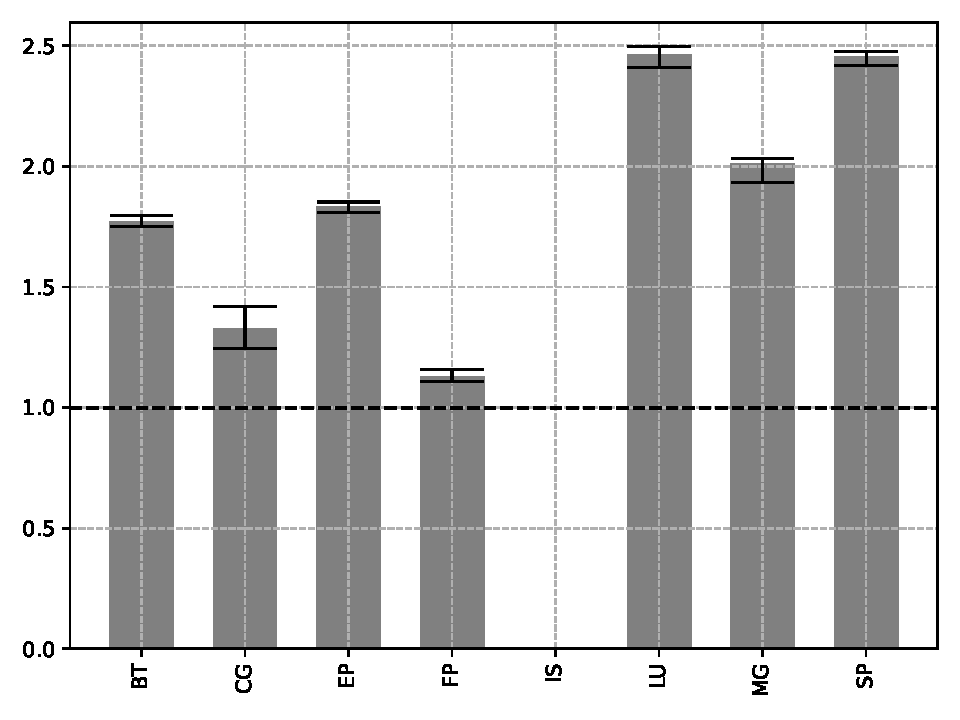
\includegraphics[width=\textwidth]
        {Images/6.1.RQ1/npb-wasmer-llvm-naive.pdf}
        \caption{NPB}
    \end{subfigure}
    \caption{Benchmarks with naive (\texttt{-O0}) on Wasmer(LLVM)}
    \label{fig:rq1-wasmer-llvm-naive}
\end{figure}

\begin{figure}
    \centering
    \begin{subfigure}[t]{\textwidth}
        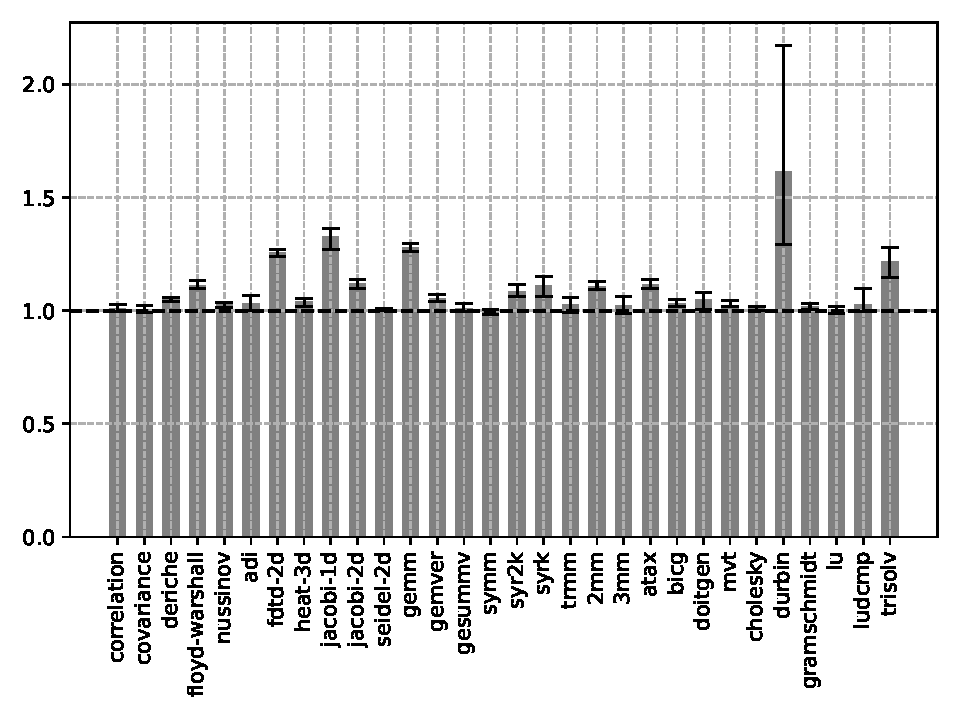
\includegraphics[width=\textwidth]
        {Images/6.1.RQ1/polybench-wasmtime-opt.pdf}
        \caption{Polybench}
        \label{fig:rq1-wasmtime-opt-polybench}
    \end{subfigure}
    \begin{subfigure}[t]{.45\textwidth}
        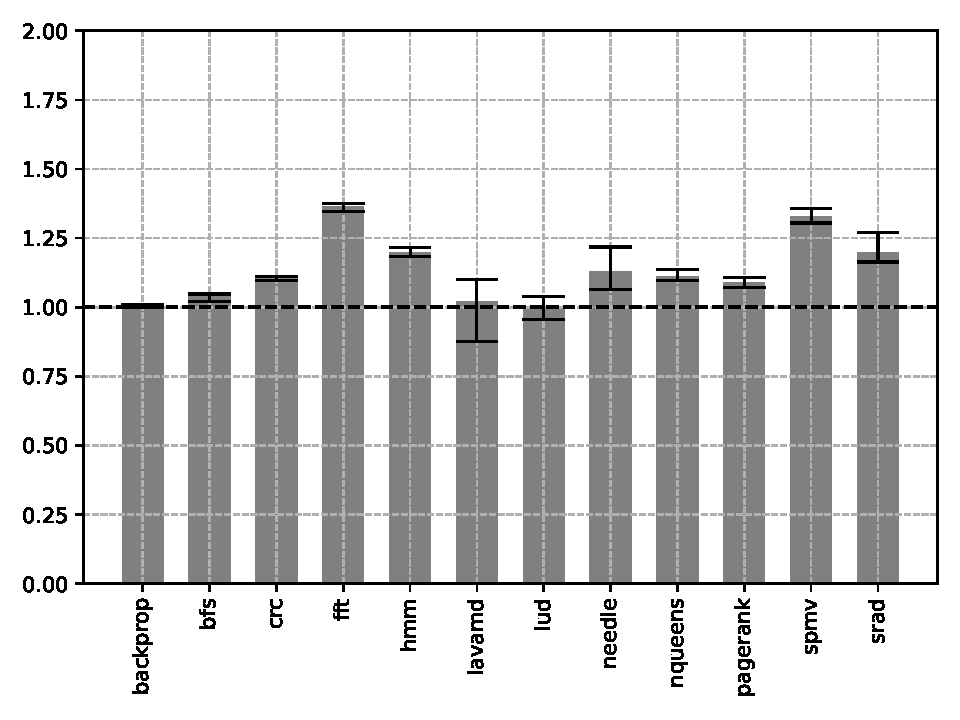
\includegraphics[width=\textwidth]
        {Images/6.1.RQ1/ostrich-wasmtime-opt.pdf}
        \caption{Ostrich}
    \end{subfigure}
    \begin{subfigure}[t]{.45\textwidth}
        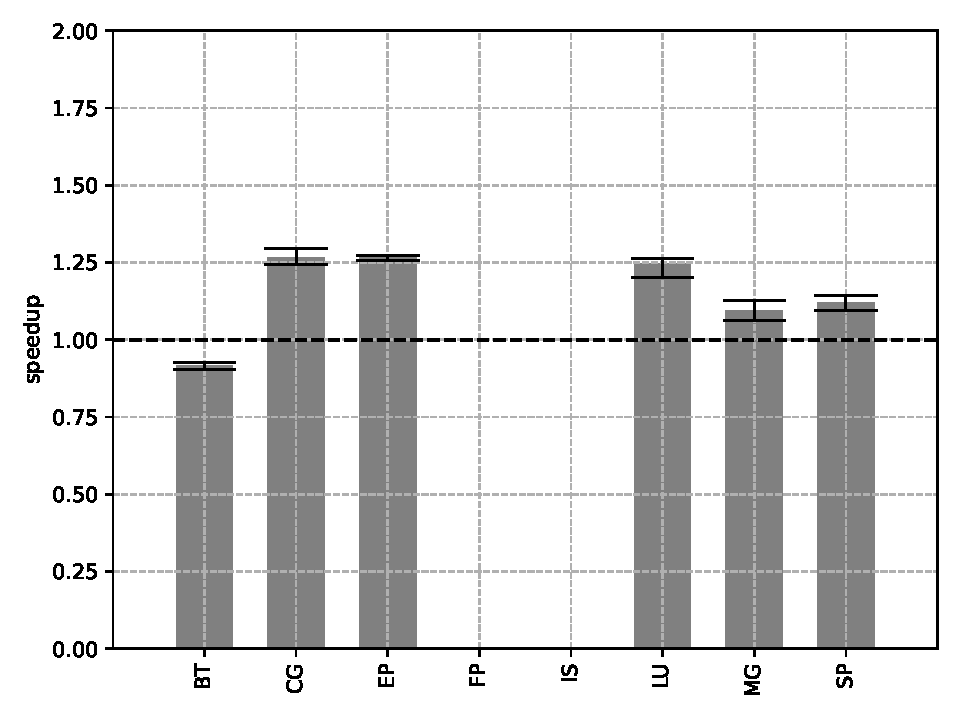
\includegraphics[width=\textwidth]
        {Images/6.1.RQ1/npb-wasmtime-opt.pdf}
        \caption{NPB}
    \end{subfigure}
    \caption{Benchmarks with optimized (\texttt{-O3}) on Wasmtime}
    \label{fig:rq1-wasmtime-opt}
\end{figure}

\begin{figure}
    \centering
    \begin{subfigure}[t]{\textwidth}
        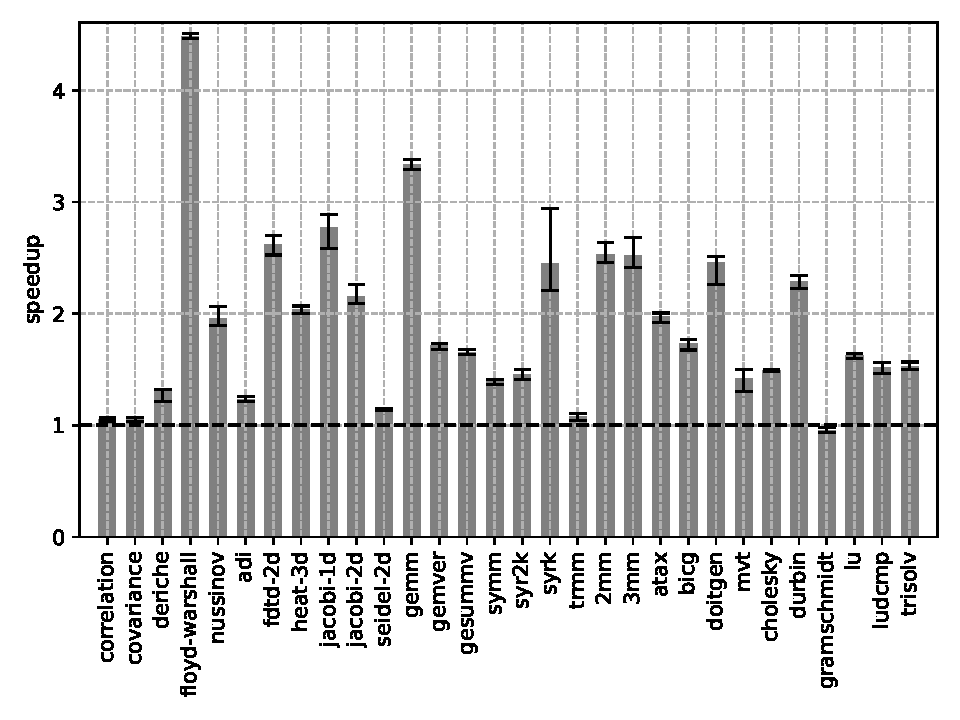
\includegraphics[width=\textwidth]
        {Images/6.1.RQ1/polybench-wasmer-cranelift-opt.pdf}
        \caption{Polybench}
    \end{subfigure}
    \begin{subfigure}[t]{.45\textwidth}
        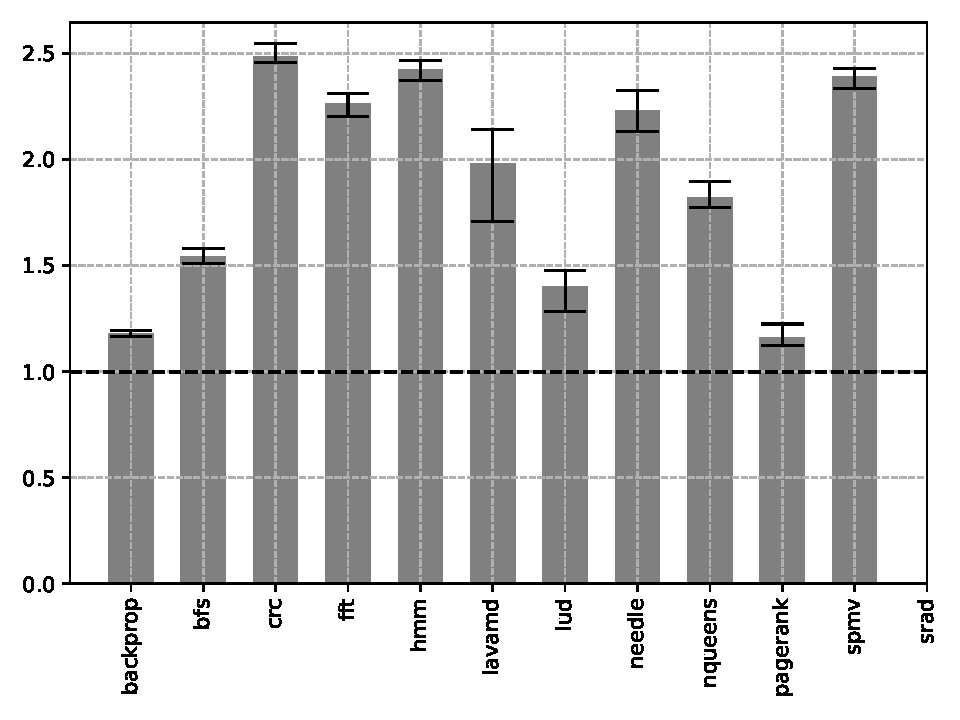
\includegraphics[width=\textwidth]
        {Images/6.1.RQ1/ostrich-wasmer-cranelift-opt.pdf}
        \caption{Ostrich}
    \end{subfigure}
    \begin{subfigure}[t]{.45\textwidth}
        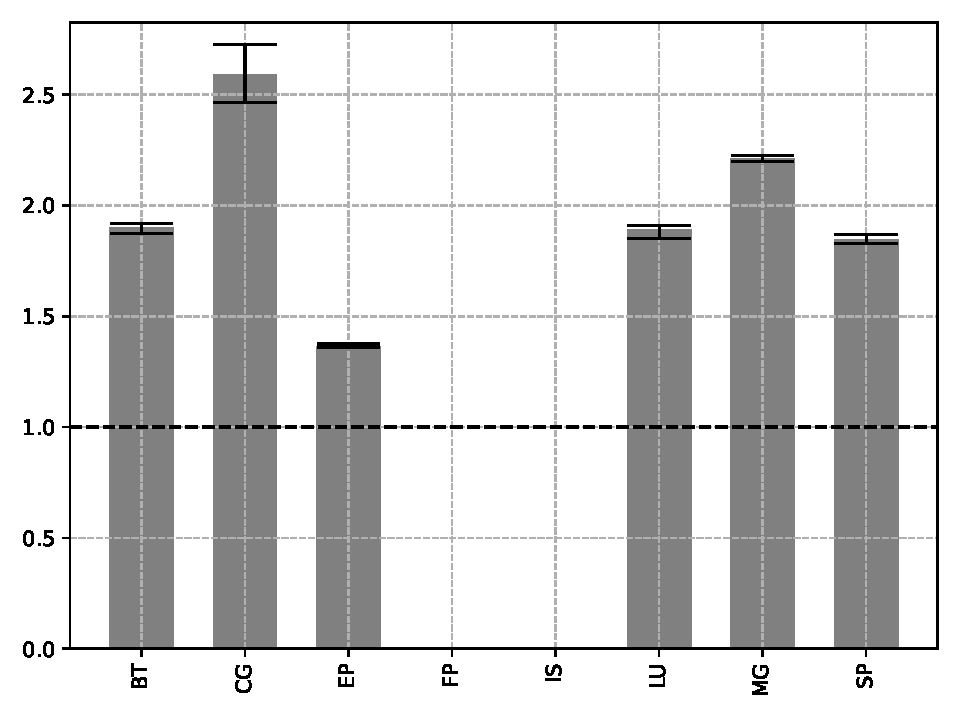
\includegraphics[width=\textwidth]
        {Images/6.1.RQ1/npb-wasmer-cranelift-opt.pdf}
        \caption{NPB}
    \end{subfigure}
    \caption{Benchmarks with optimized (\texttt{-O3}) on Wasmer(Cranelift)}
    \label{fig:rq1-wamer-cranelift-opt}
\end{figure}

\begin{figure}
    \centering
    \begin{subfigure}[t]{\textwidth}
        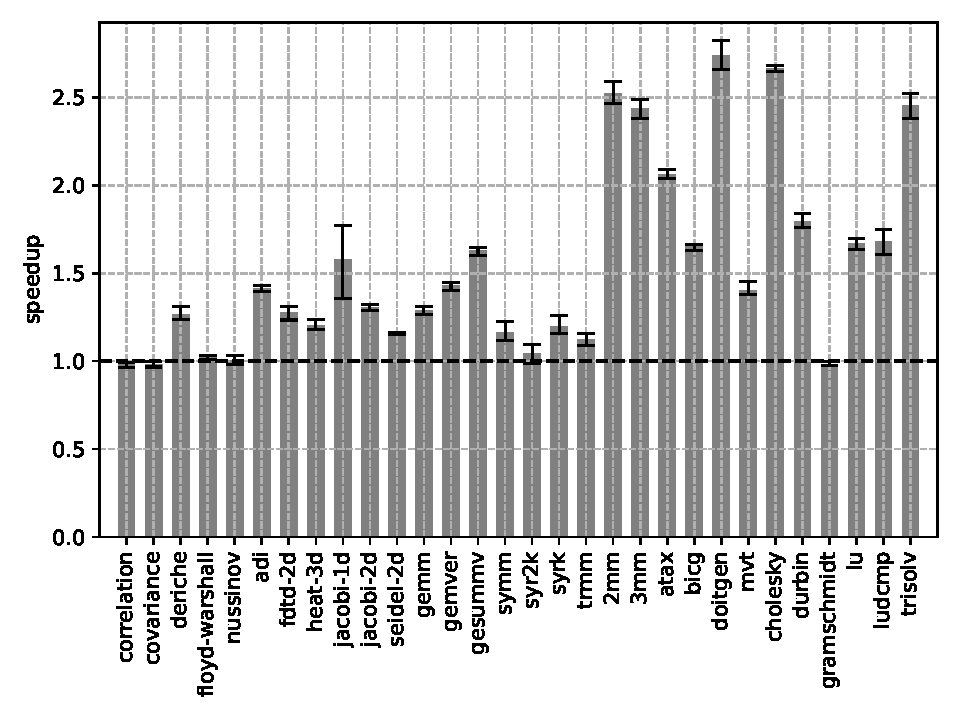
\includegraphics[width=\textwidth]
        {Images/6.1.RQ1/polybench-wasmer-llvm-opt.pdf}
        \caption{Polybench}
    \end{subfigure}
    \begin{subfigure}[t]{.45\textwidth}
        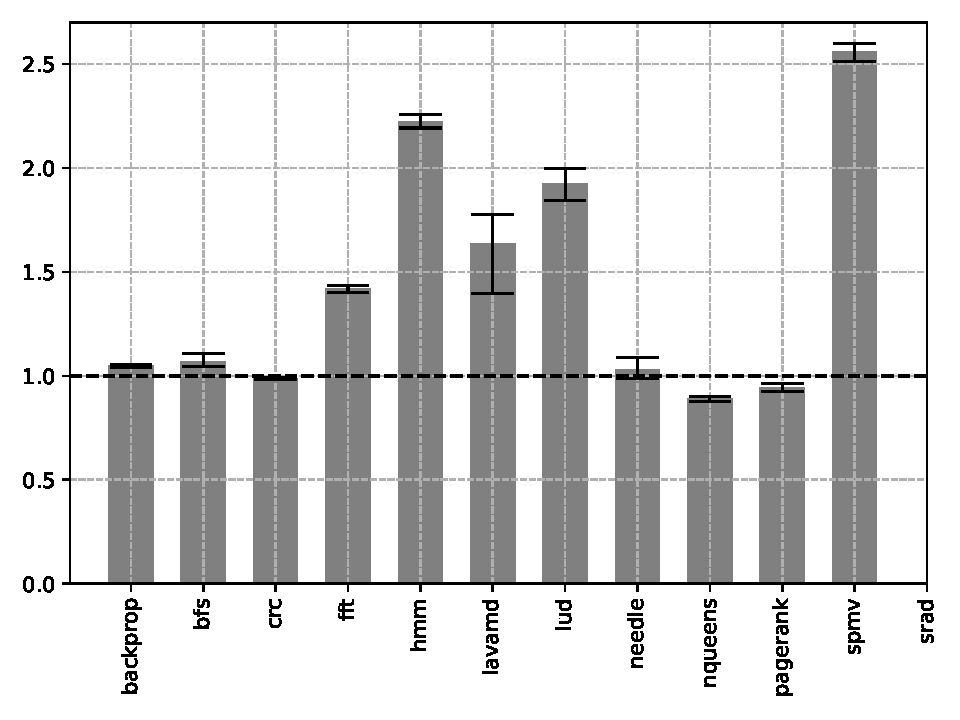
\includegraphics[width=\textwidth]
        {Images/6.1.RQ1/ostrich-wasmer-llvm-opt.pdf}
        \caption{Ostrich}
    \end{subfigure}
    \begin{subfigure}[t]{.45\textwidth}
        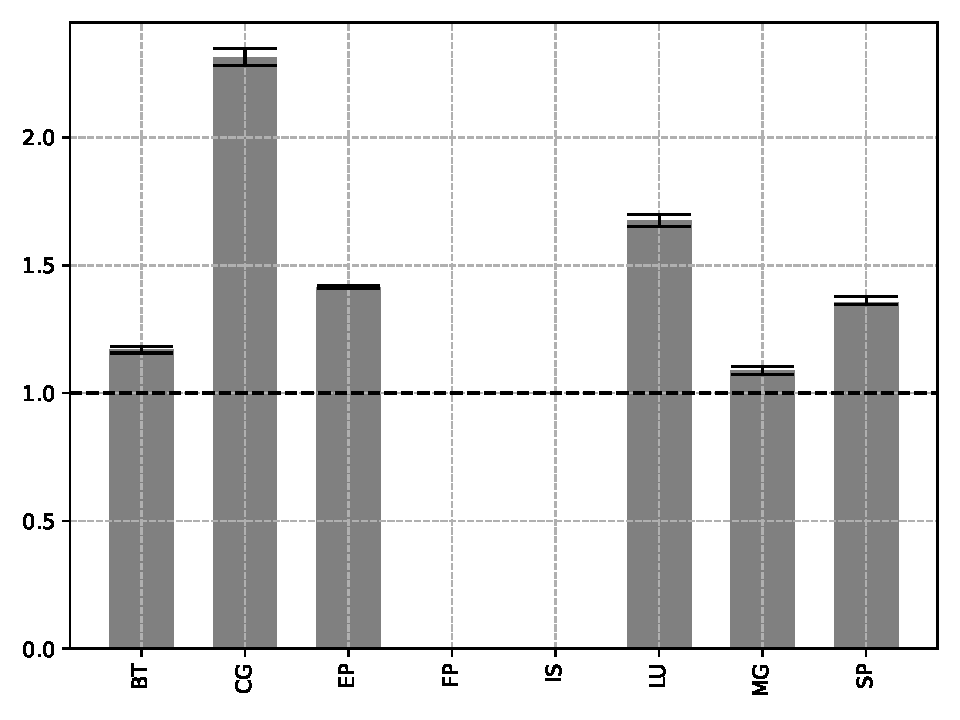
\includegraphics[width=\textwidth]
        {Images/6.1.RQ1/npb-wasmer-llvm-opt.pdf}
        \caption{NPB}
    \end{subfigure}
    \caption{Benchmarks with optimized (\texttt{-O3}) on Wasmer(LLVM)}
    \label{fig:rq1-wasmer-llvm-opt}
\end{figure}

\begin{figure}
    \centering
    \begin{subfigure}[t]{\textwidth}
        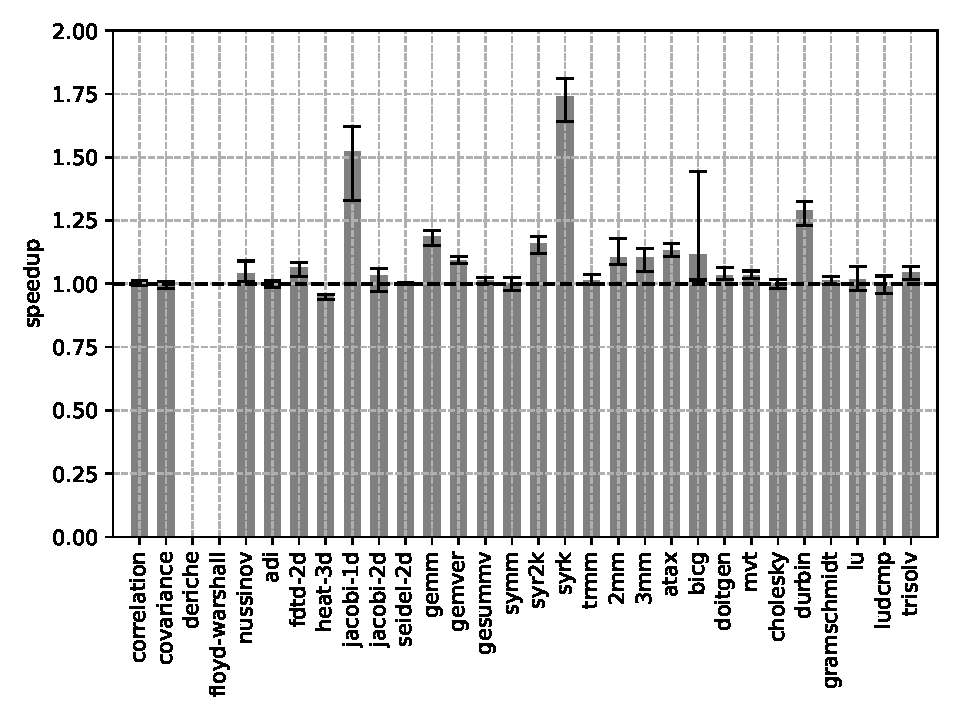
\includegraphics[width=\textwidth]
        {Images/6.1.RQ1/polybench-wasmtime-simd.pdf}
        \caption{Polybench}
    \end{subfigure}
    \begin{subfigure}[t]{.45\textwidth}
        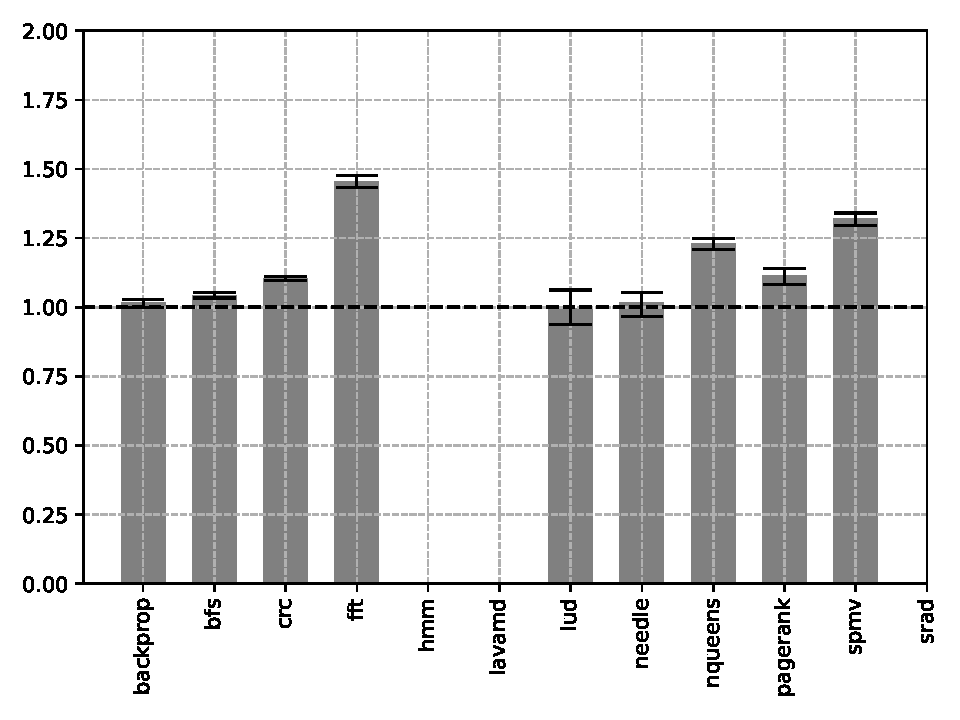
\includegraphics[width=\textwidth]
        {Images/6.1.RQ1/ostrich-wasmtime-simd.pdf}
        \caption{Ostrich}
    \end{subfigure}
    \begin{subfigure}[t]{.45\textwidth}
        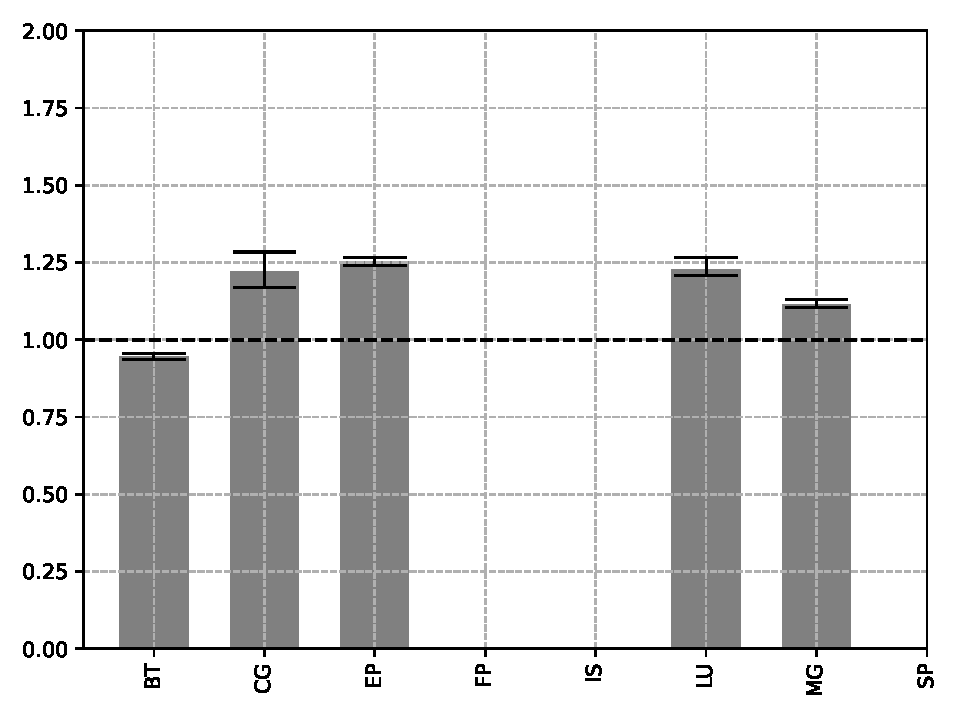
\includegraphics[width=\textwidth]
        {Images/6.1.RQ1/npb-wasmtime-simd.pdf}
        \caption{NPB}
    \end{subfigure}
    \caption{Benchmarks with SIMD extension (\texttt{-O3 -msimd128}) on Wasmtime}
    \label{fig:rq1-wasmtime-simd}
\end{figure}

\begin{figure}
    \centering
    \begin{subfigure}[t]{\textwidth}
        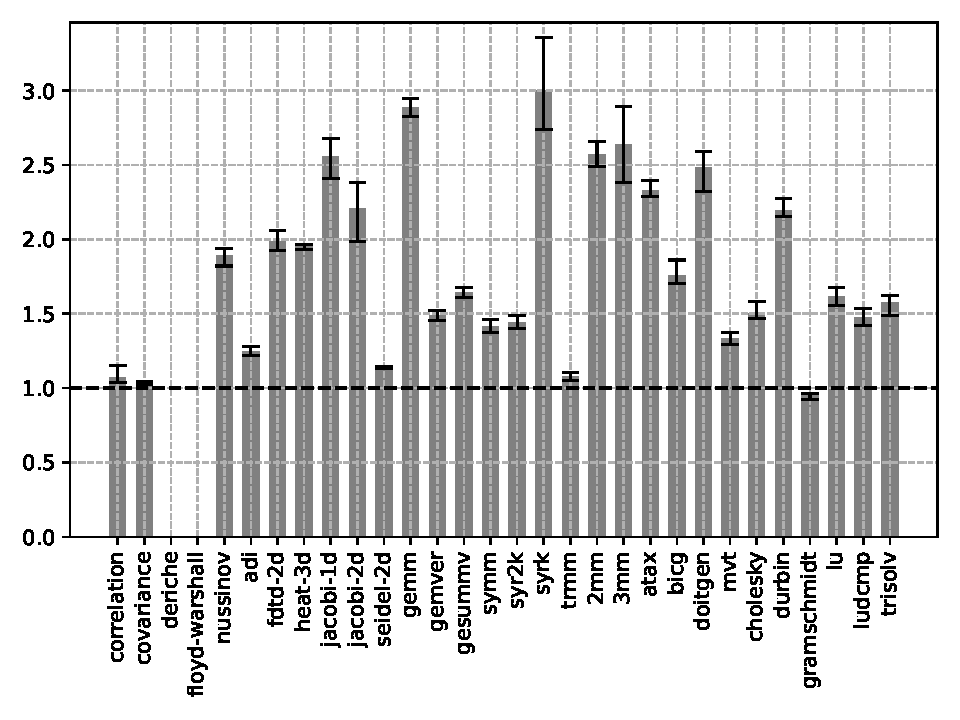
\includegraphics[width=\textwidth]
        {Images/6.1.RQ1/polybench-wasmer-cranelift-simd.pdf}
        \caption{Polybench}
    \end{subfigure}
    \begin{subfigure}[t]{.45\textwidth}
        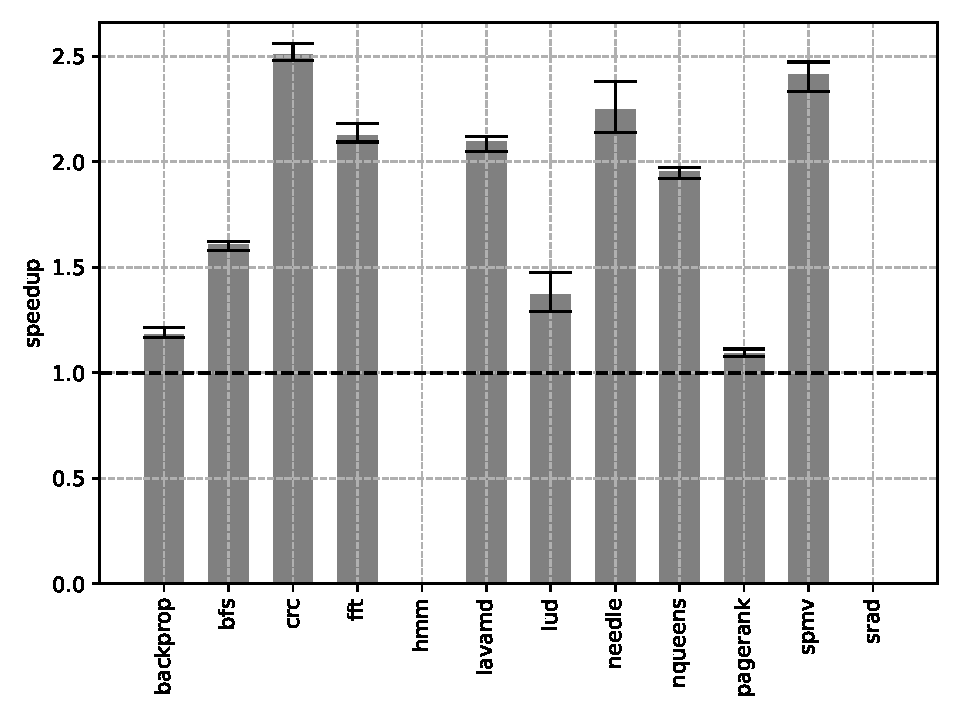
\includegraphics[width=\textwidth]
        {Images/6.1.RQ1/ostrich-wasmer-cranelift-simd.pdf}
        \caption{Ostrich}
    \end{subfigure}
    \begin{subfigure}[t]{.45\textwidth}
        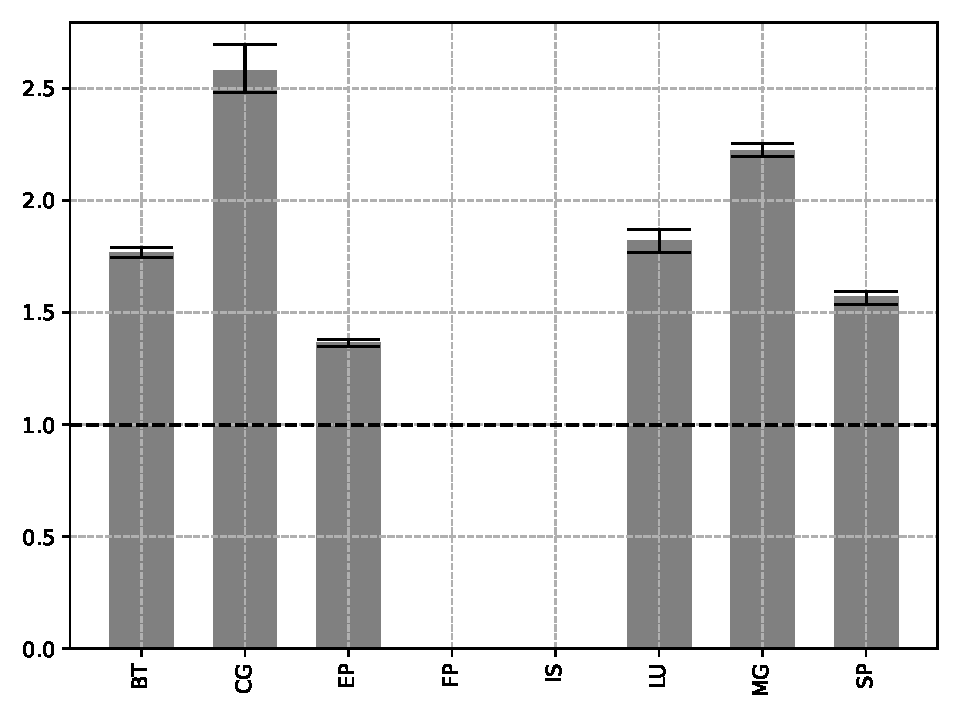
\includegraphics[width=\textwidth]
        {Images/6.1.RQ1/npb-wasmer-cranelift-simd.pdf}
        \caption{NPB}
    \end{subfigure}
    \caption{Benchmarks with SIMD extension (\texttt{-O3 -msimd128}) on Wasmer(Cranelift)}
    \label{fig:rq1-wasmer-cranelift-simd}
\end{figure}

\begin{figure}
    \centering
    \begin{subfigure}[t]{\textwidth}
        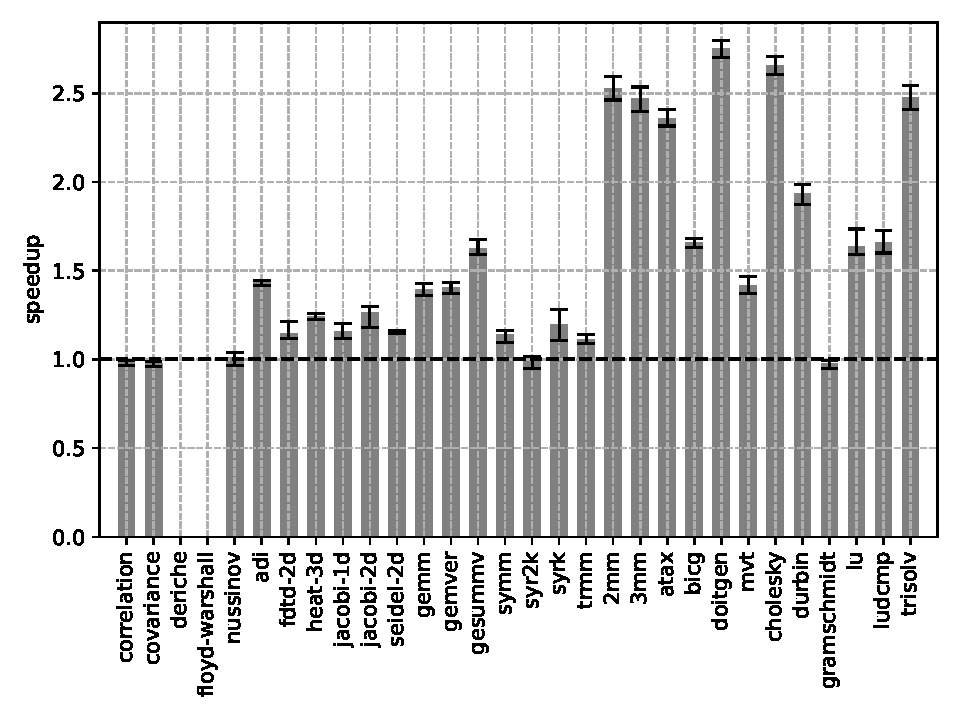
\includegraphics[width=\textwidth]
        {Images/6.1.RQ1/polybench-wasmer-llvm-simd.pdf}
        \caption{Polybench}
    \end{subfigure}
    \begin{subfigure}[t]{.45\textwidth}
        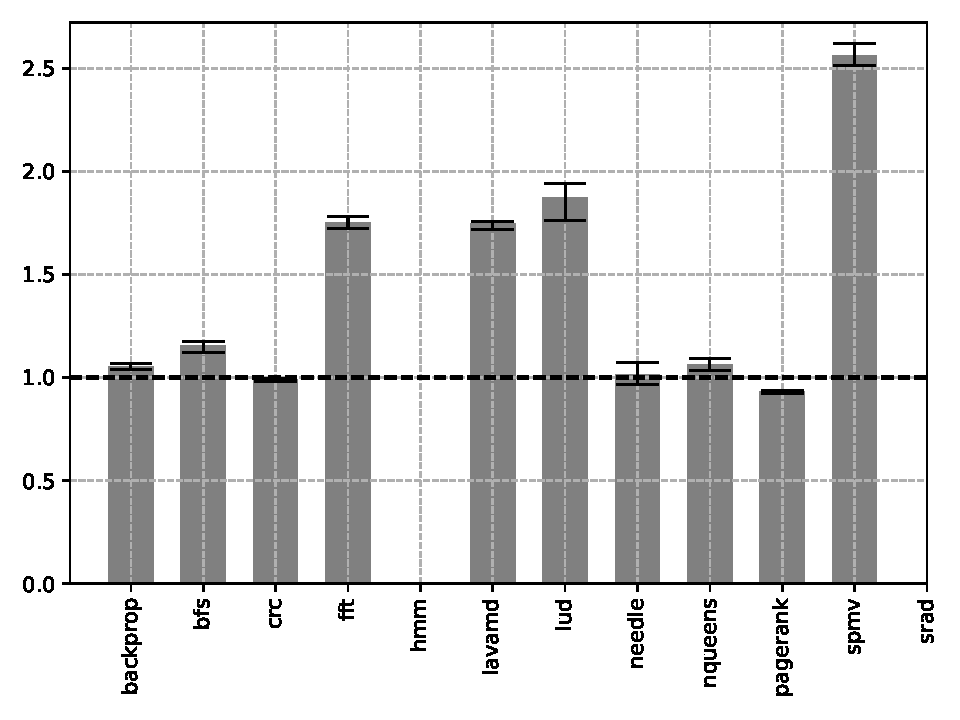
\includegraphics[width=\textwidth]
        {Images/6.1.RQ1/ostrich-wasmer-llvm-simd.pdf}
        \caption{Ostrich}
    \end{subfigure}
    \begin{subfigure}[t]{.45\textwidth}
        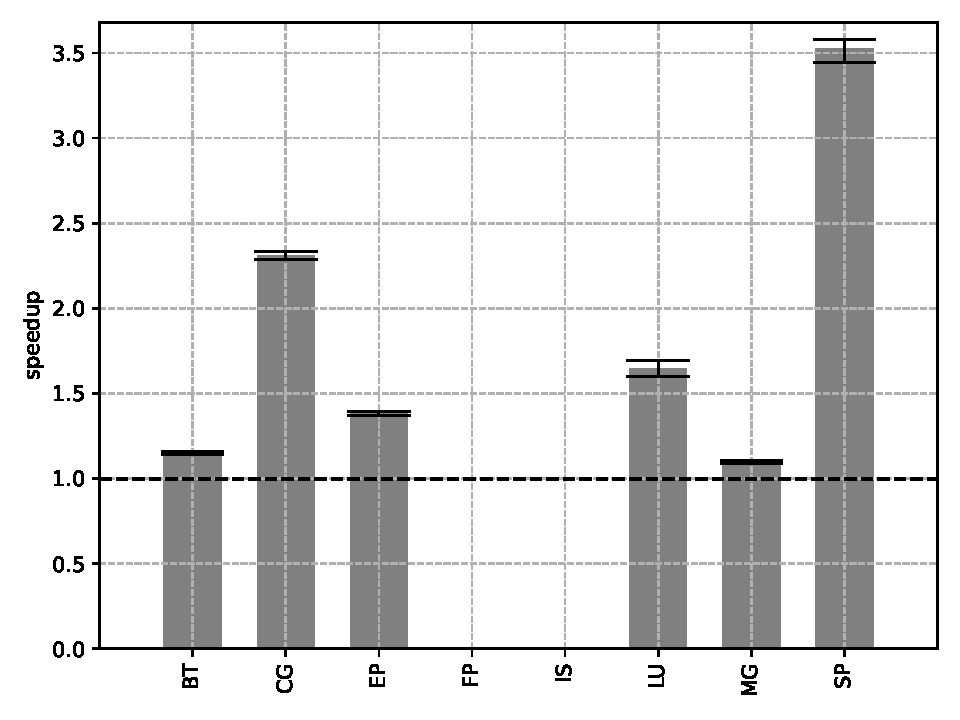
\includegraphics[width=\textwidth]
        {Images/6.1.RQ1/npb-wasmer-llvm-simd.pdf}
        \caption{NPB}
    \end{subfigure}
    \caption{Benchmarks with SIMD extension (\texttt{-O3 -msimd128}) on Wasmer(LLVM)}
    \label{fig:rq1-wasmer-llvm-simd}
\end{figure}

This section will compare SableWasm performance against several other WebAssembly runtime environments, specifically Wasmtime and Wasmer. We will benchmark three implementations over naive (\texttt{-O0}), optimized (\texttt{-O3}), and SIMD-enabled optimized (\texttt{-O3 -msimd128}) WebAssembly modules compiled from the source. One can consider Wasmtime \footnote{Wasmtime: \url{https://github.com/bytecodealliance/wasmtime}} as the `reference' implementation of WebAssembly out of the browser and maintained by the WebAssembly community group. The system is built upon the  custom compile framework, Cranelift \footnote{Cranelift: \url{https://github.com/bytecodealliance/wasmtime/tree/main/cranelift}}. Currently, both Cranelift and Wasmtime are still under active development and subject to changes in the future. Here, in this project, we anchor our Wasmtime at version 0.26.0. Wasmer \footnote{Wasmer: \url{https://wasmer.io/}} is another community approach for running WebAssembly sandboxed applications outside of the browser. It comes with a package manager, WAPM \footnote{WAPM: \url{https://wapm.io/}}, that distributes applications in WebAssembly binary module format. Wasmer supports three compiler backends, LLVM, Cranelift, and a one-pass code generator for fast compilation. In this chapter, we will focus on the LLVM and Cranelift variants of Wasmer. Similar to Wasmtime, Wasmer is also under active development at the time of thesis writing, and we fix the version of Wasmer at 1.0.2. Unlike SableWasm, an ahead-of-time(AOT) compiler for WebAssembly modules, Wasmtime and Wasmer are both just-in-time (JIT). Thus, when measuring the benchmark's performance, we need to isolate the error induced by the compiler, such as compilation-overhead and warm-up time. To eliminate the compilation-overhead, we measure the execution time within the internal timing code by issuing syscalls to the WASI layer. Further, we adjust the benchmark size for Ostrich and NPB so that each benchmark case takes more than 10 seconds to compute to reduce the error introduced by the JIT warm-up process.

Figure~\ref{fig:rq1-wasmtime-naive} to figure~\ref{fig:rq1-wasmer-llvm-simd} presents the benchmark result. We normalize the data with respect to the SableWasm's execution time and present them as speed-ups. A number higher than one means that the SableWasm's performance is better than the candidate, and on the other hand, a less than one speed-up refers to slow-down. The error bar is calculated based on the  10th percentile and 90th percentile accordingly. For naive translated WebAssembly modules, SableWasm performs better than Wasmtime in most benchmark cases but slower in seven cases in total.

For naive translated WebAssembly modules, SableWasm performs better than Wasmtime in most benchmark cases except seven of them. We suspect that slow down comes from the excessive linear memory access. In the current version of the WASI-enable Clang compiler, a naive translated module will use linear memory to simulate stack frame functions instead of using local variables. This means that when writing to a function local variable, SableWasm needs to first load the linear memory base pointer from the instance object, calculate the address and then perform the memory access. Making the case worse, the current SableWasm will always load the base memory pointer even if a local variable already holds the base pointer. LLVM cannot effectively eliminate these load instructions, as the linear memory base pointer in the instance object is volatile. One possible solution to ease the problem is to carefully annotate the instance object pointer so that the alias analysis in SableWasm can correctly identify these redundant load instructions. On the other hand, SableWasm performs better than Wasmer with both Cranelift or LLVM backend. This is quite interesting as the current SableWasm is also built upon LLVM. We suspect that two factors are contributing to the speedup. First, SableWasm employs several optimization techniques to improve the quality of the generated LLVM intermediate representation. When designing the translation patterns for lowering SableWasm MIR into LLVM IR, we notice that the quality of LLVM IR has a significant impact on the result performance, especially for auto-vectorization. Second, Wasmer supports many other safety features that are not specified in the WebAssembly specification, such as stack probing. These safety features impose performance drawbacks on the system and can be observed from the benchmark results above.

For optimized and SIMD-enabled input WebAssembly modules, SableWasm performs on par with Wasmtime, except on benchmark case \texttt{durbin}. One may also notice that the error for \texttt{durbin} in figure~\ref{fig:rq1-wasmtime-opt-polybench} is more significant compared to others. This is due to the nature of \texttt{durbin} benchmark case. For Ostrich and NPB, we can adjust the benchmark size to reduce the measurement errors. However, this is not the case for Polybench, as the input size is hardcoded. On the other hand, SableWasm performs better than Wasmer in most of the benchmark cases. Here we will take \texttt{floyd-warshall} as an example. The core computation function in \texttt{floyd-warshall} is a nested for loop that iteratively multiplies then adds matrices. This operation is highly parallel. We notice that the performance of SableWasm is approximately four times better in optimized input and two times better for SIMD-enabled. Currently, there seems no way to retrieve generated LLVM IR from Wasmer, and we can only suspect reasons based on the experiment result. We suspect that the auto-vectorization may cause this in the LLVM framework. The four times and two times speedup appears to align with the SIMD vector operations for packed double-precision floating-point numbers. Thus, Wasmer may contain awkwardly generated LLVM intermediate representation that stops auto-vectorization pass to turn scalar code into the vectorized form.

\begin{table}
    \centering
    % Please add the following required packages to your document preamble:
% \usepackage{multirow}
% \usepackage[table,xcdraw]{xcolor}
% If you use beamer only pass "xcolor=table" option, i.e. \documentclass[xcolor=table]{beamer}

\begin{tabular}{ll|ccc}
    \multicolumn{2}{c|}{\textbf{Benchmark name}}                 & \textbf{Wasmtime}                   & \textbf{Wasmer (Cranelift)} & \textbf{Wasmer (LLVM)}                                    \\ \hline
    \rowcolor[HTML]{C0C0C0}
    \cellcolor[HTML]{C0C0C0}                                     & Naive                               & 1.19                        & 3.18                        & 1.50                        \\
    \rowcolor[HTML]{C0C0C0}
    \cellcolor[HTML]{C0C0C0}                                     & Optimized                           & 1.09                        & 1.90                        & 1.54                        \\
    \rowcolor[HTML]{C0C0C0}
    \multirow{-3}{*}{\cellcolor[HTML]{C0C0C0}\textbf{Polybench}} & SIMD-enabled                        & 1.10                        & 1.80                        & 1.56                        \\ \hline
                                                                 & Naive                               & 1.07                        & 2.43                        & 1.34                        \\
                                                                 & Optimized                           & 1.13                        & 1.90                        & 1.43                        \\
    \multirow{-3}{*}{\textbf{Ostrich}}                           & SIMD-enabled                        & 1.14                        & 1.86                        & 1.41                        \\ \hline
    \rowcolor[HTML]{C0C0C0}
    \cellcolor[HTML]{C0C0C0}                                     & {\color[HTML]{333333} Naive}        & {\color[HTML]{333333} 1.23} & {\color[HTML]{333333} 3.42} & {\color[HTML]{333333} 1.86} \\
    \rowcolor[HTML]{C0C0C0}
    \cellcolor[HTML]{C0C0C0}                                     & {\color[HTML]{333333} Optimized}    & {\color[HTML]{333333} 1.15} & {\color[HTML]{333333} 1.97} & {\color[HTML]{333333} 1.50} \\
    \rowcolor[HTML]{C0C0C0}
    \multirow{-3}{*}{\cellcolor[HTML]{C0C0C0}\textbf{NPB}}       & {\color[HTML]{333333} SIMD-enabled} & {\color[HTML]{333333} 1.15} & {\color[HTML]{333333} 1.89} & {\color[HTML]{333333} 1.85}
\end{tabular}

    \caption{Average speedups compare to Wasmtime and Wasmer}
    \label{tbl:rq1-average}
\end{table}

In general, we conclude that SableWasm performs on par with Wasmtime on optimized and SIMD-enabled WebAssembly modules and better than Wasmtime and Wasmer for other benchmark cases, as shown in table~\ref{tbl:rq1-average}.


\section[RQ2: Does optimization over input modules matter?]{
  {\large RQ2: Does optimization over input modules matter?}}

\begin{figure}
    \centering
    \begin{subfigure}[t]{\textwidth}
        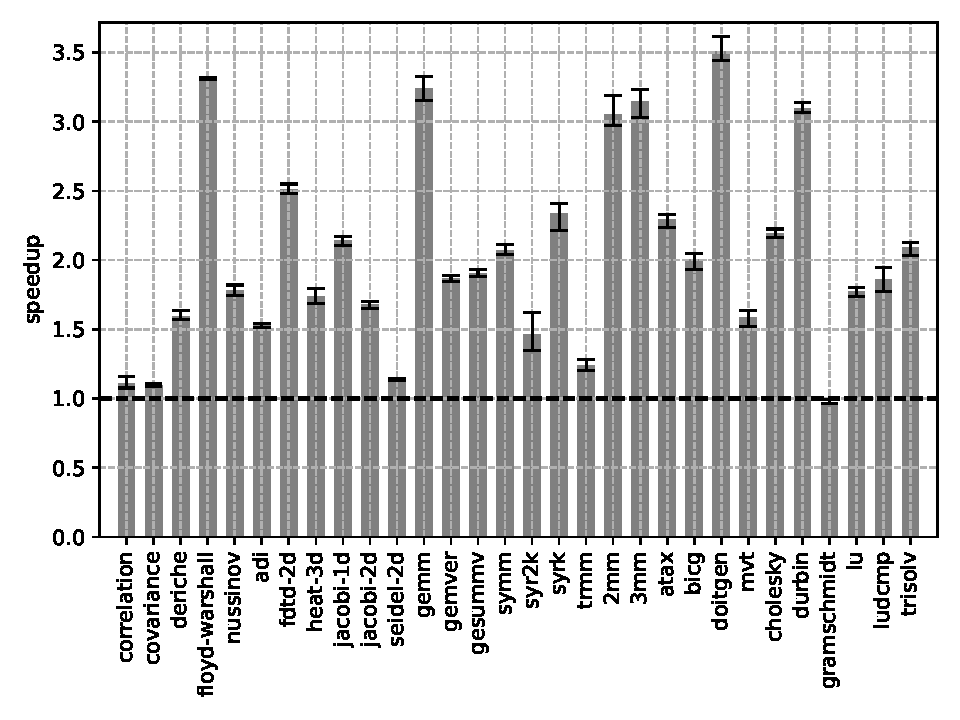
\includegraphics[width=\textwidth]{Images/6.2.RQ2/polybench-opt-speedup}
        \caption{Polybench}
    \end{subfigure}
    \begin{subfigure}[t]{.45\textwidth}
        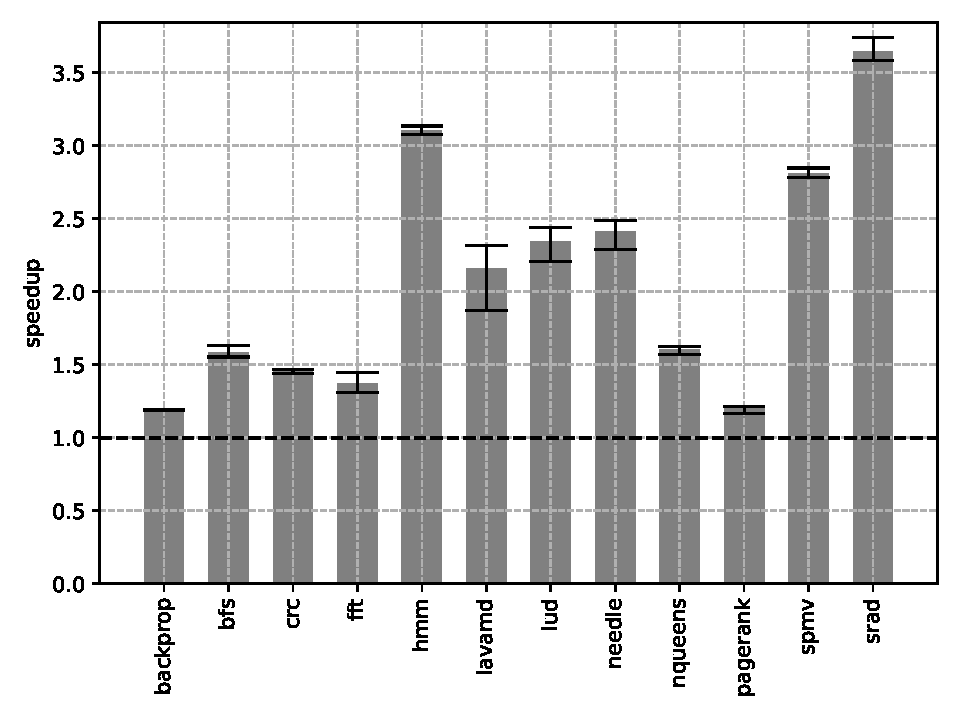
\includegraphics[width=\textwidth]{Images/6.2.RQ2/ostrich-opt-speedup}
        \caption{Ostrich}
    \end{subfigure}
    \begin{subfigure}[t]{.45\textwidth}
        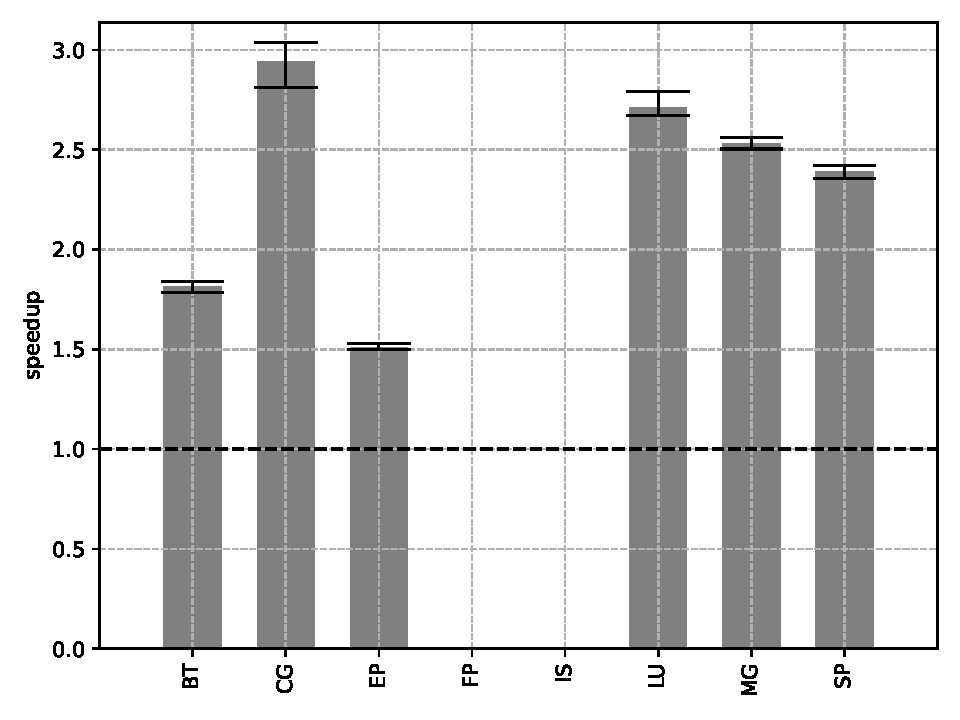
\includegraphics[width=\textwidth]{Images/6.2.RQ2/npb-opt-speedup}
        \caption{NPB}
    \end{subfigure}
    \caption{Comparision between optimized and naive input modules}
    \label{fig:rq2}
\end{figure}

The second problem we would like to investigate in the thesis is whether the optimization over input WebAssembly modules affects their performance in SableWasm. In theory, a perfect runtime system should recover all the missed possible optimization from a naive translated WebAssembly module, which we have seen in many other systems with two-phase compilation. The most well-known example is perhaps Java. The first compiler, \texttt{javac}, translates Java source files into bytecodes, and on the other hand, the Java virtual machine (JVM) generates naive executable binaries based on the bytecodes. \texttt{javac} will translate the source files faithfully, without complex transformation and optimization, while JVM optimizes the bytecodes effectively.  This design helps the system to achieve fast compilation while ensures the quality of the final generated code. Unfortunately, in the current SableWasm, the optimization over input WebAssembly modules does have a significant impact on the overall performance. When investigating the problem, we compare the SableWasm execution time under naive translated WebAssembly modules against their optimized counterparts.

For most of the benchmarks, except \texttt{gramschmidt}, we have seen a significant performance increase for optimized WebAssembly modules, as shown in figure~\ref{fig:rq2}. Here we will take \texttt{trisolv} as an example. We found many optimizations missing when comparing the LLVM intermediate representation generated from a naive WebAssembly module against an optimized one. The most notable difference is perhaps function inlining and loop unrolling. In LLVM generated by naive WebAssembly module, SableWasm does not inline the primary function \texttt{kernel\_trisolv} into the main function. Thus, matrix size is pass through as arguments to the computation kernel, which holds back SableWasm from unrolling the internal nested for loops. We suspect that the translation patterns used in SableWasm when lowering WebAssembly bytecode into SableWasm MIR confuse the LLVM backend. Another interesting question is why \texttt{gramschmidt} has similar performance on both input WebAssembly modules. When we compare the LLVM intermediate representation for both inputs, we found that SableWasm can recover nearly all the optimization in the computation kernel. Additionally, the computation kernel for \texttt{gramschmidt} is extremely simple, only consisting of three non-nested for loops. This further confirms our theory on performance difference.

\section[RQ3: How much does SIMD extension improve in performance?]{
  {\large RQ3: How much does SIMD extension improve in performance?}}

\begin{figure}
    \centering
    \begin{subfigure}[t]{\textwidth}
        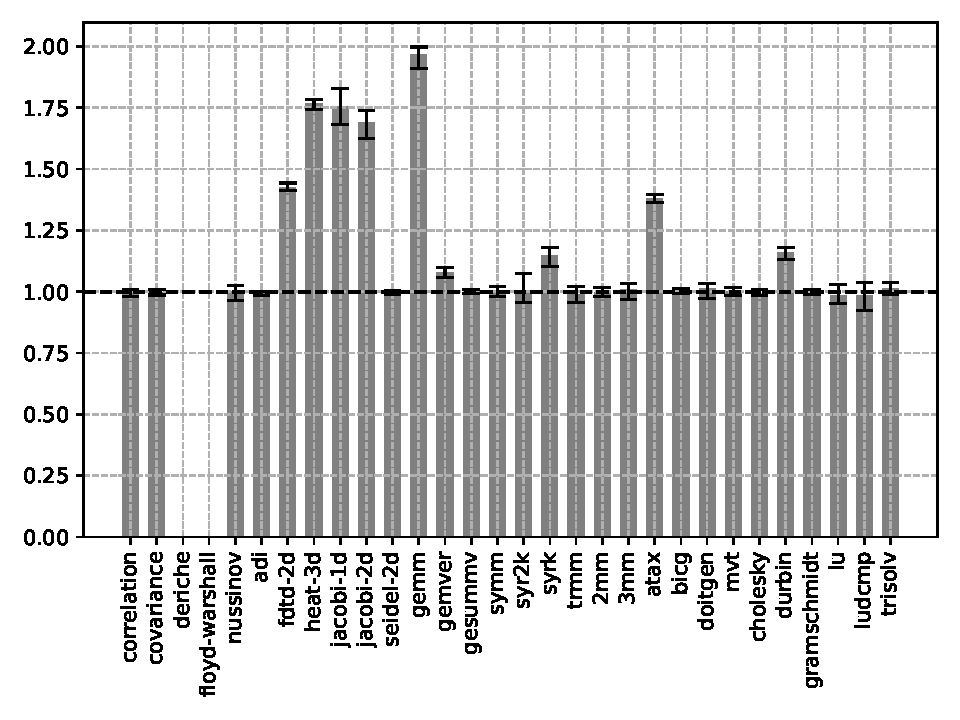
\includegraphics[width=\textwidth]{Images/6.3.RQ3/polybench-simd-speedup}
        \caption{Polybench}
    \end{subfigure}
    \begin{subfigure}[t]{.45\textwidth}
        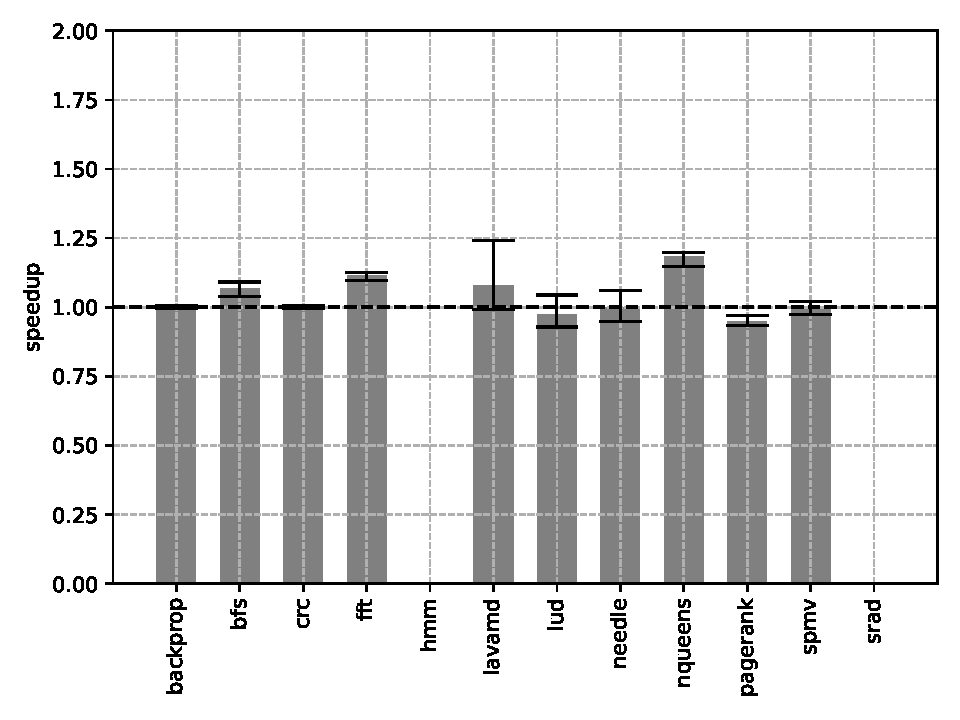
\includegraphics[width=\textwidth]{Images/6.3.RQ3/ostrich-simd-speedup}
        \caption{Ostrich}
    \end{subfigure}
    \begin{subfigure}[t]{.45\textwidth}
        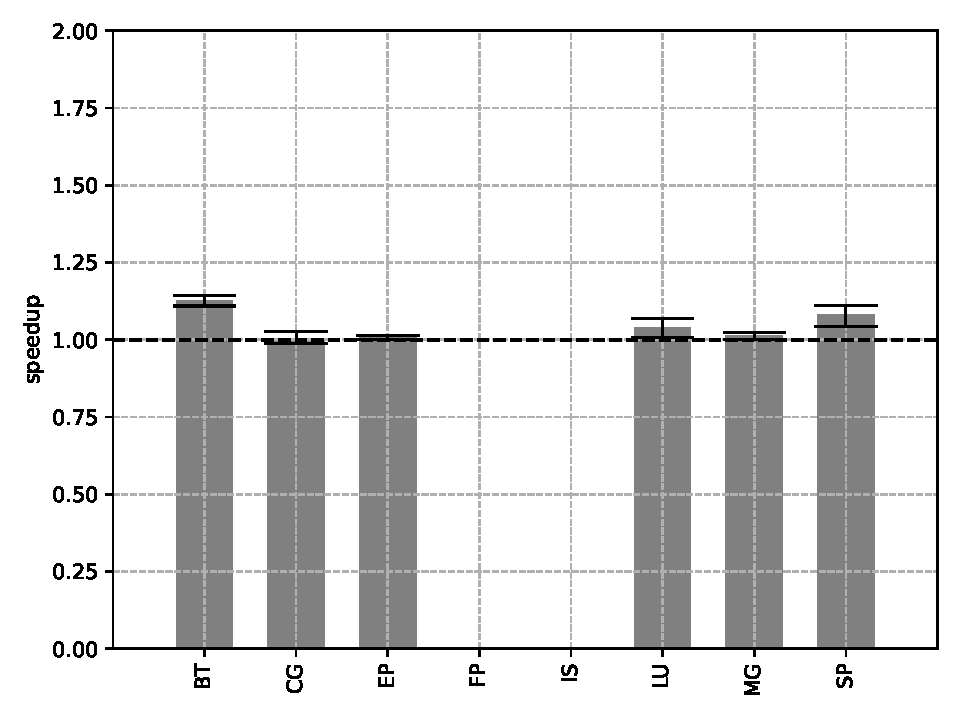
\includegraphics[width=\textwidth]{Images/6.3.RQ3/npb-simd-speedup}
        \caption{NPB}
    \end{subfigure}
    \caption{Comparision between SIMD-enabled and optimized input modules}
    \label{fig:rq3}
\end{figure}

\begin{figure}
    \centering
    \begin{subfigure}{\textwidth}
        \lstinputlisting[basicstyle=\linespread{0.5}\ttfamily\small, language=LLVM, numbers=left]{Code/6.Evaluation/gemm.opt.ll}
        \caption{Optimized}
        \label{fig:polybench-gemm-opt-code}
    \end{subfigure}
    \begin{subfigure}{\textwidth}
        \lstinputlisting[basicstyle=\linespread{0.5}\ttfamily\small, language=LLVM, numbers=left]{Code/6.Evaluation/gemm.simd.ll}
        \caption{SIMD-enabled}
        \label{fig:polybench-gemm-simd-code}
    \end{subfigure}
    \caption{Polybench \texttt{gemm} code snippet}
\end{figure}

\begin{figure}
    \lstinputlisting[language=C, basicstyle=\linespread{0.8}\ttfamily\small, numbers=left]{Code/6.Evaluation/gemm.kernel.c}
    \caption{Polybench \texttt{gemm} benchmark kernel}
    \label{fig:polybench-gemm-kernel}
\end{figure}

The last question we would like to investigate in the thesis is how much WebAssembly SIMD operation extension improves performance compared to MVP WebAssembly. In this experiment, we compare the execution time between optimized WebAssembly modules and SIMD-enabled WebAssembly modules. Figure~\ref{fig:rq3} illustrates the experiment results. For most benchmark cases, the SIMD extension does not significantly improve the performance, except five in Polybench. Here we will take \texttt{gemm} as an example. Figure~\ref{fig:polybench-gemm-kernel} illustrates the computation kernel of the benchmark, and it consists of a single nested loop that performs floating-point mathematics over two matrics. When SableWasm translation the optimized (\texttt{-O3}) input WebAssembly module, illustrated in figure~\ref{fig:polybench-gemm-opt-code}, it correctly performs loop interleaving on the inner for loop. However, the LLVM auto-vectorizer failed to transform the scalar code into a parallel form. On the other hand, in the case of SIMD-enabled WebAssembly module input (\texttt{-O3 -msimd128}), SableWasm takes the direct hint from the WASI-enabled clang compiler and correctly emit the 128-bit wide vector operations. We suspect that the frontend WASI-enable Clang compiler recognize the vectorizable pattern in both case, however, in the optimized (\texttt{-O3}), it scalarized the already vectorized code due to the limitations of the instruction set.

\chapter{Related Work}
\chapter{Future Work and Conclusion}
\label{chapter:conclusion}

WebAssembly has been growing in popularity in recent years as a new format
for distributing sandboxed applications over the internet. In this project, we
presented SableWasm as a standalone ahead-of-time (AOT) compiler for
translating WebAssembly modules into shared libraries. We also implement a
runtime environment that enables other programming languages such as C/C++ to
interact with generated shared libraries.

We first started the project with a custom parser for WebAssembly binary format.
The parser focuses on extensibility and performance, as currently, WebAssembly
is still under the standardization process and several syntax extensions might
be merged to the specification soon. We then evaluate the performance of the
parser by benchmarking against \texttt{wabt}, the reference implementation
provided by the WebAssembly community, and observe a 1.6x speedup in execution
speed and a 4.6x reduction in memory footprint.

We then define the middle-level representation (MIR) for SableWasm. SableWasm
MIR is a register-based control flow graph representation of the WebAssembly
program. When translating WebAssembly bytecode to SableWasm MIR, we focus on
two significant problems. First, WebAssembly is a stack-based bytecode with
structured control flow structures. Thus, to faithfully translate the bytecode,
we define translation patterns that mimic the semantics of these constructs and
reduce them into basic blocks and branching instructions. The other problem we
encountered is regarding the size of the instruction set. As WebAssembly encodes
both type and shape information in the instruction opcode, the WebAssembly
instruction set is quite large. Additionally, to reduce the size of the module,
WebAssembly fuses several typical instruction sequences into one single
instruction, such as load-and-extend. To maintain a small instruction set, we
define several reduction rules for WebAssembly instructions. Unfortunately,
these translation patterns lead to awkward and inefficient code. To address
this problem, we implement an analysis and transformation framework over
SableWasm MIR. We then design simplifying control flow graph pass that
incrementally improves the MIR, similar to a `peephole optimization' by
locating and replacing several common redundant patterns.

The last component of SableWasm is the SableWasm runtime library, which provides
implementations for builtin functions used in the generated shared libraries.
It also implements several WebAssembly entities, such as the linear memory and
the indirect table. Currently, the SableWasm runtime library defines an
easy-to-use C/C++ interface to the user and handles errors and exceptions
using the exception mechanism in C++.

Finally, we evaluate SableWasm's performance by benchmarking with three
well-known benchmark suites, Polybench, Ostrich, and NPB. The first question
we focus on in this thesis is how SableWasm performs compared to other existing
WebAssembly runtime environments. We conclude that SableWasm performs on par
with Wasmtime and approximately 1.5x to 2x faster than Wasmer. The second
research question is whether optimization over input WebAssembly modules
affects the overall performance in SableWasm. By comparing the execution time
of SableWasm under optimized translated input modules against that of naive
translated input modules, we conclude that, currently, optimization over the
WebAssembly modules has a significant impact on the performance. Hence, when
designing frontend compilers that target WebAssembly, one should be careful of
translation patterns and perform optimizations as early as possible. The last
question we investigated in this thesis is whether the WebAssembly SIMD
extension brings performance improvement to SableWasm. Experimentally, we can
see significant benefit. However, using Polybench, we locate many common
patterns that cannot be identified and rewritten by LLVM's auto-vectorizer
in SableWasm.

\section*{Future Work}

WebAssembly is a relatively new language, and many of its features are still
under the standardization phase. SableWasm only covers several WebAssembly
extensions such as the multi-value extension and the SIMD operation extension.
One excellent opportunity is to implement more WebAssembly extensions in
SableWasm, such as the garbage collection (GC) extension and the exception
handling extension. Currently, many high-level languages, such as
AssemblyScript, require static linking with a non-trivial runtime library when
cross-compiling into WebAssembly. Simulating these features results in notable
increases in code size and a slow down in performance.

Another interesting direction is to add more analysis and transformation in
SableWasm under the optimization framework. More specifically, one can implement
an auto-vectorizer in SableWasm at the MIR level. The evaluation chapter shows
that the LLVM's auto-vectorizer cannot recognize many apparent patterns and
yields inefficient code. We suspect that the boilerplate code introduced by
the translation patterns confuses the auto-vectorizer. Hence, an auto-vectorizer
at the SableWasm MIR level can better understand the program and, in theory,
recover more opportunities within the WebAssembly modules.

Finally, one can also add more backend support for SableWasm. Currently,
SableWasm is an ahead-of-time (AOT) compiler built on the LLVM compiler
infrastructure. One natural extension of this project to implement a
just-in-time (JIT) system that uses LLVM's Orc JIT framework. Additionally,
one can also explore many profile-guided optimizations (PGO) techniques used
in many other VM languages, such as Java bytecode \cite{java-pgo}.

\bibliography{references}
\bibliographystyle{acm}

\end{document}